\documentclass[11pt,a4paper]{article}
\usepackage[utf8]{inputenc}
\usepackage[margin=2.5cm]{geometry}
\usepackage{iohk}
\usepackage{microtype}
\usepackage{mathpazo} % nice fonts
\usepackage{amsmath}
\usepackage{amssymb}
\usepackage{latexsym}
\usepackage{mathtools}
\usepackage{stmaryrd}
\usepackage{extarrows}
\usepackage{slashed}
\usepackage[colon]{natbib}
\usepackage[unicode=true,pdftex,pdfa,colorlinks=true]{hyperref}
\usepackage{xcolor}
\usepackage[capitalise,noabbrev,nameinlink]{cleveref}
\usepackage{float}
\floatstyle{boxed}
\restylefloat{figure}
\usepackage{listings} % for code blocks.
%%
%% Package `semantic` can be used for writing inference rules.
%%
\usepackage{semantic}
%% Setup for the semantic package
\setpremisesspace{20pt}
\usepackage{tikz}
\usetikzlibrary{decorations.pathreplacing, positioning, arrows.meta, calc}
% For drawing simple diagrams involving arrows between LaTeX symbols
\usepackage{tikz-cd}

%%
%% Types
%%
\newcommand{\Bool}{\type{Bool}}
\newcommand{\Tx}{\type{Tx}}
\newcommand{\Ix}{\type{Ix}}
\newcommand{\TxId}{\type{TxId}}
\newcommand{\Addr}{\type{Addr}}
\newcommand{\UTxO}{\type{UTxO}}
\newcommand{\Value}{\type{Value}}
\newcommand{\Lovelace}{\type{Lovelace}}
\newcommand{\UTxOEnv}{\type{UTxOEnv}}
\newcommand{\UTxOState}{\type{UTxOState}}
%% Adding witnesses
\newcommand{\TxIn}{\type{TxIn}}
\newcommand{\TxOut}{\type{TxOut}}
\newcommand{\VKey}{\type{VKey}}
\newcommand{\SKey}{\type{SKey}}
\newcommand{\KeyHash}{\type{KeyHash}}
\newcommand{\SkVk}{\type{SkVk}}
\newcommand{\Sig}{\type{Sig}}
\newcommand{\Data}{\type{Data}}
%% Adding delegation
\newcommand{\Epoch}{\type{Epoch}}
\newcommand{\VKeyGen}{\type{VKey_G}}
%% Blockchain
\newcommand{\Gkeys}{\var{G_{keys}}}
\newcommand{\Block}{\type{Block}}
\newcommand{\CEEnv}{\type{CEEnv}}
\newcommand{\CEState}{\type{CEState}}
\newcommand{\BDEnv}{\type{BDEnv}}
\newcommand{\BDState}{\type{BDState}}
\newcommand{\Slot}{\type{Slot}}
\newcommand{\SlotCount}{\type{SlotCount}}

%%
%% Functions
%%
\newcommand{\txins}[1]{\fun{txins}~ \var{#1}}
\newcommand{\txid}[1]{\fun{txid}~ \var{#1}}
\newcommand{\txouts}[1]{\fun{txouts}~ \var{#1}}
\newcommand{\values}[1]{\fun{values}~ #1}
\newcommand{\balance}[1]{\fun{balance}~ \var{#1}}
%% UTxO witnesses
\newcommand{\inputs}[1]{\fun{inputs}~ \var{#1}}
\newcommand{\wits}[1]{\fun{wits}~ \var{#1}}
\newcommand{\verify}[3]{\fun{verify} ~ #1 ~ #2 ~ #3}
\newcommand{\sign}[2]{\fun{sign} ~ #1 ~ #2}
\newcommand{\serialised}[1]{\llbracket \var{#1} \rrbracket}
\newcommand{\addr}[1]{\fun{addr}~ \var{#1}}
\newcommand{\hash}[1]{\fun{hash}~ \var{#1}}
\newcommand{\txbody}[1]{\fun{txbody}~ \var{#1}}
\newcommand{\txfee}[1]{\fun{txfee}~ \var{#1}}
\newcommand{\minfee}[2]{\fun{minfee}~ \var{#1}~ \var{#2}}
% wildcard parameter
\newcommand{\wcard}[0]{\underline{\phantom{a}}}
%% Adding ledgers...
\newcommand{\utxo}[1]{\fun{utxo}~ #1}
%% Delegation
\newcommand{\delegatesName}{\fun{delegates}}
\newcommand{\delegates}[3]{\delegatesName~#1~#2~#3}
\newcommand{\dwho}[1]{\fun{dwho}~\var{#1}}
\newcommand{\depoch}[1]{\fun{depoch}~\var{#1}}
%% Delegation witnesses
\newcommand{\dbody}[1]{\fun{dbody}~\var{#1}}
\newcommand{\dwit}[1]{\fun{dwit}~\var{#1}}
%% Blockchain
\newcommand{\bwit}[1]{\fun{bwit}~\var{#1}}
\newcommand{\bslot}[1]{\fun{bslot}~\var{#1}}
\newcommand{\bbody}[1]{\fun{bbody}~\var{#1}}
\newcommand{\bdlgs}[1]{\fun{bdlgs}~\var{#1}}
%% Set notation
\newcommand\Set[2]{\{\,#1\mid#2\,\}}
%% Let bindings
\newcommand{\leteq}{\ensuremath{\mathrel{\mathop:}=}}

%% For properties
\newcommand{\txs}{\ensuremath{\mathcal{T}}}
\newcommand{\transtar}[2]{\xlongrightarrow[\textsc{#1}]{#2}\negthickspace^{*}}
\newcommand{\biguo}[1]{\ensuremath{\underset{#1}{\underrightarrow\bigcup}}}

%\includeonly{update-mechanism, delegation, blockchain-interface}

%% Parameters that control floats placement. See https://robjhyndman.com/hyndsight/latex-floats/
\setcounter{topnumber}{2}
\setcounter{bottomnumber}{2}
\setcounter{totalnumber}{4}
\renewcommand{\topfraction}{0.85}
\renewcommand{\bottomfraction}{0.85}
\renewcommand{\textfraction}{0.15}
\renewcommand{\floatpagefraction}{0.7}
\newcommand{\DEnv}{\type{DEnv}}
\newcommand{\DSEnv}{\type{DSEnv}}
\newcommand{\DSState}{\type{DSState}}
\newcommand{\DCert}{\type{DCert}}
\newcommand{\DState}{\type{DState}}
\newcommand{\DEState}{\type{DEState}}


\newtheorem{definition}{Definition}
\newtheorem{property}{Property}

\begin{document}

\hypersetup{
  pdftitle={A Formal Specification of the Cardano Ledger (Byron Release)},
  breaklinks=true,
  bookmarks=true,
  colorlinks=false,
  linkcolor={blue},
  citecolor={blue},
  urlcolor={blue},
  linkbordercolor={white},
  citebordercolor={white},
  urlbordercolor={white}
}

\title{
  A Formal Specification of the Cardano Ledger\\
  \small{(for the Byron release)}
}

\author{Damian Nadales \\
  {\small \texttt{damian.nadales@iohk.io}}\\
}

\date{\today}

\maketitle

\begin{abstract}
  This document defines the rules for extending a ledger with transactions, as
  implemented in the Byron release of the Cardano Ledger. It is intended to
  serve as the specification for random generators of transactions which adhere
  to the rules presented here.
\end{abstract}

\section*{List of Contributors}
\label{acknowledgements}

Jared Corduan, Nicholas Clarke, Marko Dimjašević, Duncan Coutts, Ru Horlick,
Michael Hueschen, Ryan Lemmer.


\tableofcontents
\listoffigures

\section{Introduction}
\label{sec:introduction-shelley}

This document is a formal specification of the functionality of the ledger on the blockchain.
This includes the blockchain layer determining what is a valid block,
but does not include any concurrency issues such as chain selection.
The details of the background and the larger context
for the design decisions formalized in this document are presented
in~\cite{delegation_design}.

In this document,
we present the most important properties that any implementation of the ledger must have.
Specifically, we model the following aspects
of the functionality of the ledger on the blockchain:

\begin{description}
\item[Preservation of value] Every coin in the system must be accounted for,
  and the total amount is unchanged by every transaction and epoch change.
  In particular, every coin is accounted for by exactly one of the following categories:
  \begin{itemize}
    \item Circulation (UTxO)
    \item Deposit pot
    \item Fee pot
    \item Reserves (monetary expansion)
    \item Rewards (account addresses)
    \item Treasury
  \end{itemize}
\item[Witnesses] Authentication of parts of the transaction data by means of
  cryptographic entities (such as signatures and private keys) contained in
  these transactions.
\item[Delegation] Validity of delegation certificates, which delegate
  block-signing rights.
\item[Stake] Staking rights associated to an address.
\item[Rewards] Reward calculation and distribution.
\item[Updates] The update mechanism for Shelley protocol parameters and software.
\end{description}

While the blockchain protocol is a reactive system that is driven by the arrival
of blocks causing updates to the ledger, the formal description is a collection
of rules that compose a
static description of what a \textit{valid ledger} is. A valid ledger state can only
be reached by applying a sequence of inference rules and any valid ledger state
is reachable by applying some sequence of these rules.
The specifics of the semantics we use to define and apply
the rules we present in this document are explained in detail in
\cite{small_step_semantics} (this document will really help the reader's
understanding of the contents of this specification).

The structure of the rules that we give here is such that their application is
deterministic. That is, given a specific initial state and relevant environmental
constants, there is no ambiguity
about which rule should be applied at any given time (i.e.~which state
transition is allowed to take place). This property ensures that the specification
is totally precise --- no
choice is left to the implementor and any two implementations must
behave the same when it comes to deciding whether a block is valid.


\section{Notation}
\label{sec:notation-shelley}

The transition system is explained in \cite{small_step_semantics}.

\begin{description}
  \item[Powerset] Given a set $\type{X}$, $\powerset{\type{X}}$ is the set of all
    the subsets of $\type{X}$.
  \item[Sequences] Given a set $\type{X}$, $\seqof{\type{X}}$ is the set of
    sequences having elements taken from $\type{X}$. The empty sequence is
    denoted by $\epsilon$. Given a sequence $\Lambda$, $\Lambda; \type{x}$ is
    the sequence that results from appending $\type{x} \in \type{X}$ to
    $\Lambda$.
  \item[Functions] $A \to B$ denotes a \textbf{total function} from $A$ to $B$.
    Given a function $f$ we write $f~a$ for the application of $f$ to argument
    $a$.
  \item[Inverse Image] Given a function $f: A \to B$ and $b\in B$, we write
    $f^{-1}~b$ for the \textbf{inverse image} of $f$ at $b$, which is defined by
    $\{a \mid\ f a =  b\}$.
  \item[Maps and partial functions] $A \mapsto B$ denotes a \textbf{partial
    function} from $A$ to $B$, which can be seen as a map (dictionary) with
    keys in $A$ and values in $B$. Given a map $m \in A \mapsto B$, notation
    $a \mapsto b \in m$ is equivalent to $m~ a = b$. 
    The $\emptyset$ symbol is also used to
    represent the empty map as well.
  \item[Map Operations] Figure~\ref{fig:notation:nonstandard}
    describes some non-standard map operations.
  \item[Relations] A relation on $A\times B$ is a subset of $A\times B$.
    Both maps and functions can be thought of as relations.
    A function $f:A\to B$ is a relation consisting of pairs $(a, f(a))$ such that $a\in A$.
    A map $m: A\mapsto B$ is a relation consisting of pairs $(a, b)$ such that
    $a\mapsto b \in m$.
    Given a relation $R$ on $A\times B$, we define the inverse relation $R^{-1}$ to be
    all pairs $(b, a)$ such that $(a, b)\in R$. Similarly, given a function $f:A\to B$ we
    define the inverse relation $f^{-1}$ to consist of all pairs $(f(a), a)$.
    Finally, given two relations $R\subseteq A\times B$ and $S\subseteq B\times C$,
    we define the compostion $R\circ S$ to be all pairs $(a, c)$ such that
    $(a, b)\in R$ and $(b, c)\in S$ for some $b\in B$.
  \item[Option type] An option type in type $A$ is denoted as $A^? = A + \Nothing$. The
    $A$ case corresponds to the case when there is a value of type $A$ and the $\Nothing$
    case corresponds to the case when there is no value.
  \item[:=] We abuse the \textbf{:=} symbol here to mean propositional equality. In the
  style of semantics we use in this formal spec, definitional equality is not needed.
  It is meant to make the spec easier to read in the sense that each time we use it,
  we use a fresh variable as shorthand notation for an expression, e.g. we write

  \[s := slot + \StabilityWindow\]

  Then, in subsequent expressions, it is more convenient to write simply $s$.
  It is not meant to shadow variables, and if it does, there is likely a problem with the
  rules that must be addressed.
\end{description}


In Figure~\ref{fig:notation:nonstandard}, we specify the notation that we use in
the rest of the document.

\begin{figure}[htb]
  \begin{align*}
    \var{set} \restrictdom \var{map}
    & = \{ k \mapsto v \mid k \mapsto v \in \var{map}, ~ k \in \var{set} \}
    & \text{domain restriction}
    \\
    \var{set} \subtractdom \var{map}
    & = \{ k \mapsto v \mid k \mapsto v \in \var{map}, ~ k \notin \var{set} \}
    & \text{domain exclusion}
    \\
    \var{map} \restrictrange \var{set}
    & = \{ k \mapsto v \mid k \mapsto v \in \var{map}, ~ v \in \var{set} \}
    & \text{range restriction}
    \\
    \var{map} \subtractrange \var{set}
    & = \{ k \mapsto v \mid k \mapsto v \in \var{map}, ~ v \notin \var{set} \}
    & \text{range exclusion}
    \\
    A \triangle B
    & = (A \setminus B) \cup (B \setminus A)
    & \text{symmetric difference}
    \\
    M \unionoverrideRight N
    & = (\dom N \subtractdom M)\cup N
    & \text{union override right}
    \\
    M \unionoverrideLeft N
    & = M \cup (\dom M \subtractdom N)
    & \text{union override left}
    \\
    M \unionoverridePlus N
    & = (M \triangle N)
    \cup \{k\mapsto v_1+v_2\mid {k\mapsto v_1}\in M \land {k\mapsto v_2}\in N \}
    & \text{union override plus} \\
    & & \text{(for monoidal values)}\\
  \end{align*}
  \caption{Non-standard map operators}
  \label{fig:notation:nonstandard}
\end{figure}

\clearpage


\section{Cryptographic primitives}
\label{sec:crypto-primitives-shelley}

Figure~\ref{fig:crypto-defs-shelley} introduces the cryptographic abstractions used in
this document. We begin by listing the abstract types, which are meant to
represent the corresponding concepts in cryptography.
Their exact
implementation remains open to interpretation and we do not rely on
any additional properties of public key cryptography that are not explicitly stated
in this document. The types and rules we give here are needed in
order to guarantee certain security properties of the delegation process, which
we discuss later.

The cryptographic concepts required for the formal definition of witnessing
include public-private key pairs, one-way functions, signatures and
multi-signature scripts. The constraint we introduce states that a signature of
some data signed with a (private) key is only correct whenever we can verify it
using the corresponding public key.

Abstract data types in this paper are essentially placeholders with names
indicating the data types they are meant to represent in an implementation.
Derived types are made up of data structures (i.e.~products, lists, finite
maps, etc.) built from abstract types. The underlying structure of a data type
is implementation-dependent and furthermore, the way the data is stored on
physical storage can vary as well.

Serialization is a physical manifestation of data on a given storage device.
In this document, the properties and rules we state involving serialization are
assumed to hold true independently of the storage medium and style of data
organization chosen for an implementation.
The type $\Ser$ denotes the serialized representation of a term of any serializable
type.

\begin{figure}[htb]
  \emph{Abstract types}
  %
  \begin{equation*}
    \begin{array}{r@{~\in~}lr}
      \var{sk} & \SKey & \text{private signing key}\\
      \var{vk} & \VKey & \text{public verifying key}\\
      \var{hk} & \KeyHash & \text{hash of a key}\\
      \sigma & \Sig  & \text{signature}\\
      \var{d} & \Ser  & \text{data}\\
      \var{script} & \Script & \text{multi-signature script} \\
      \var{hs} & \HashScr & \text{hash of a script}
    \end{array}
  \end{equation*}
  \emph{Derived types}
  \begin{equation*}
    \begin{array}{r@{~\in~}lr}
      (sk, vk) & \KeyPair & \text{signing-verifying key pairs}
    \end{array}
  \end{equation*}
  \emph{Abstract functions}
  %
  \begin{equation*}
    \begin{array}{r@{~\in~}lr}
      \hashKey{} & \VKey \to \KeyHash
                 & \text{hash a verification key} \\
                 %
      \fun{verify} & \powerset{\left(\VKey \times \Ser \times \Sig\right)}
                   & \text{verification relation}\\
                   %
      \fun{sign} & \SKey \to \Ser \to \Sig
                 & \text{signing function}\\
      \fun{hashScript} & \Script \to \HashScr & \text{hash a serialized script}
    \end{array}
  \end{equation*}
  \emph{Constraints}
  \begin{align*}
    & \forall (sk, vk) \in \KeyPair,~ d \in \Ser,~ \sigma \in \Sig \cdot
    \sign{sk}{d} = \sigma \implies (vk, d, \sigma) \in \fun{verify}
  \end{align*}
  \emph{Notation for serialized and verified data}
  \begin{align*}
    & \serialised{x} ~\in \Ser & \text{serialised representation of } x\\
    & \mathcal{V}_{\var{vk}}{\serialised{d}}_{\sigma} = \verify{vk}{d}{\sigma}
    & \text{shorthand notation for } \fun{verify}
  \end{align*}
  \caption{Cryptographic definitions}
  \label{fig:crypto-defs-shelley}
\end{figure}

When we get to the blockchain layer validation, we will use
key evolving signatures (KES).
This is another asymmetric key cryptographic scheme, also relying on
the use of public and private key pairs.
These signature schemes provide forward cryptographic security, meaning that a
compromised key does not make it easier for an adversary to forge a signature that
allegedly had been signed in the past.
Figure~\ref{fig:kes-defs-shelley} introduces the additional cryptographic abstractions
needed for KES.

In KES, the public verification key stays constant, but the
corresponding private key evolves incrementally. For this reason, KES
signing keys are indexed by integers representing the step in the key's
evolution. This evolution step parameter is also an additional parameter needed
for the signing (denoted by $\fun{sign_{ev}}$) and verification
(denoted by $\fun{verify_{ev}}$) functions.

Since the private key evolves incrementally in a KES scheme, the ledger rules
require the pool operators to evolve their keys every time a certain number of
slots have passed, as determined by the global constant $\SlotsPerKESPeriod$.

\begin{figure}[htb]
  \emph{Abstract types}
  %
  \begin{equation*}
    \begin{array}{r@{~\in~}lr}
      \var{sk} & \N \to \SKeyEv & \text{private signing keys}\\
      \var{vk} & \VKeyEv & \text{public verifying key}\\
    \end{array}
  \end{equation*}
  \emph{Notation for evolved signing key}
  \begin{align*}
    & \var{sk_n} = \var{sk}~n & n\text{-th evolution of }sk
  \end{align*}
  \emph{Derived types}
  \begin{equation*}
    \begin{array}{r@{~\in~}lr}
      (sk_n, vk) & \KeyPairEv & \text{signing-verifying key pairs}
    \end{array}
  \end{equation*}
  \emph{Abstract functions}
  %
  \begin{equation*}
    \begin{array}{r@{~\in~}lr}
      \fun{verify_{ev}} & \powerset{\left(\VKey \times \N \times \Ser \times \Sig\right)}
                        & \text{verification relation}\\
                        %
      \fun{sign_{ev}} & (\N \to \SKeyEv) \to \N \to \Ser \to \Sig
                      & \text{signing function}\\
    \end{array}
  \end{equation*}
  \emph{Constraints}
  \begin{align*}
    & \forall n\in\N, (sk_n, vk) \in \KeyPairEv, ~ d \in \Ser,~ \sigma \in \Sig \cdot \\
    & ~~~~~~~~\fun{sign_{ev}}~{sk}~{n}~{d} = \sigma \implies \verifyEv{vk}{n}{d}{\sigma}
  \end{align*}
  \emph{Notation for verified KES data}
  \begin{align*}
    & \mathcal{V}^{\mathsf{KES}}_{\var{vk}}{\serialised{d}}_{\sigma}^n
        = \verifyEv{vk}{n}{d}{\sigma}
    & \text{shorthand notation for } \fun{verify_{ev}}
  \end{align*}
  \caption{KES Cryptographic definitions}
  \label{fig:kes-defs-shelley}
\end{figure}

Figure~\ref{fig:types-msig} shows the types for multi-signature
schemes. Multi-signatures effectively specify one or more combinations of
cryptographic signatures which are considered valid. This is realized in a
native way via a script-like DSL which allows for defining terms that can be
evaluated. Multi-signature scripts is the only type of script (for any
purpose, including output-locking) that exist in Shelley.

The terms form a tree like structure and are evaluated via the
\fun{evalMultiSigScript} function. The parameters are a script and a set of key
hashes. The function returns $\mathsf{True}$ when the supplied key hashes are
a valid combination for the script, otherwise it returns $\mathsf{False}$.
The following are the four constructors that make up the multisignature script
scheme:

\begin{itemize}
\item[$\type{RequireSig}$] ~:~ the signature of a key with a specific
hash is required;
\item[$\type{RequireAllOf}$] ~:~signatures of all of the keys that hash to the
values specified in the given list are required;
\item[$\type{RequireAnyOf}$] ~:~a single signature is required, by a key hashing
to one of the given values in the list (this constructor is redundant and can
be expressed using $\type{RequireMOf}$);
\item[$\type{RequireMOf}$]~:~ $m$ of the keys with the hashes specified in the list
are required to sign
\end{itemize}

\begin{figure*}[hbt]
  \emph{MultiSig Type}

  \begin{equation*}
    \begin{array}{rll}
      \MSig & \subseteq & \Script \\
      \\~\\
      \var{msig}\in\MSig & = & \type{RequireSig}~\KeyHash\\
      & \uniondistinct &
         \type{RequireAllOf}~[\Script] \\
      & \uniondistinct&
         \type{RequireAnyOf}~[\Script] \\
      & \uniondistinct&
        \type{RequireMOf}~\N~[\Script]
    \end{array}
  \end{equation*}

  \emph{Functions}

  \begin{align*}
    \fun{evalMultiSigScript} & \in\MSig\to\powerset\KeyHash\to\Bool & \\
    \fun{evalMultiSigScript} & ~(\type{RequireSig}~hk)~\var{vhks} =  hk \in vhks \\
    \fun{evalMultiSigScript} & ~(\type{RequireAllOf}~ts)~\var{vhks} =
                              \forall t \in ts: \fun{evalMultiSigScript}~t~vhks\\
    \fun{evalMultiSigScript} & ~(\type{RequireAnyOf}~ts)~\var{vhks} =
                              \exists t \in ts: \fun{evalMultiSigScript}~t~vhks\\
    \fun{evalMultiSigScript} & ~(\type{RequireMOf}~m~ts)~\var{vhks} = \\
                             & m \leq \Sigma
                               \left(
                               [\textrm{if}~(\fun{evalMultiSigScript}~\var{t}~\var{vhks})~
                               \textrm{then}~1~\textrm{else}~0\vert t \leftarrow ts]
                               \right)
  \end{align*}

  \caption{Multi-signature via Native Scripts}
  \label{fig:types-msig}
\end{figure*}


%\subsection{Verifiable Random Functions (VRF)}
%\label{sec:defs-vrf}
Figure~\ref{fig:defs-vrf} shows the cryptographic abstractions needed for Verifiable Random Functions (VRF). VRFs allow key-pair owners, $(sk, vk)\in \KeyPair$, to evaluate a pseudorandom function in a provable way given a randomness seed. Any party with access to the verification key, $vk$, the randomness seed, the proof and the generated randomness can indeed verify that the value is pseudorandom. 

\begin{figure}[htb]
  %
  \emph{Abstract types}
  \begin{equation*}
    \begin{array}{r@{~\in~}lr}
      \var{seed} & \Seed  & \text{seed for pseudo-random number generator}\\
      \var{prf} & \Proof  & \text{VRF proof}\\
    \end{array}
  \end{equation*}
  %
  \emph{Abstract functions ($T$ an arbitrary type)}
  %
  \begin{equation*}
    \begin{array}{r@{~\in~}lr}
      \seedOp & \Seed \to \Seed \to \Seed & \text{binary seed operation} \\
      \vrf{\T}{}{} & \SKey \to \Seed \to \T\times\Proof
                   & \text{verifiable random function} \\
                   %
      \verifyVrf{\T}{}{}{} & \VKey \to \Seed \to \Proof\times\T \to \Bool
                           & \text{verify vrf proof} \\
                           %
    \end{array}
  \end{equation*}
  %
  \emph{Derived Types}
  \begin{align*}
    \PoolDistr = \KeyHash_{pool} \mapsto \left([0, 1]\times\KeyHash_{vrf}\right)
      \text{ \hspace{1cm}stake pool distribution}
  \end{align*}
  %

  \emph{Constraints}
  \begin{align*}
    & \forall (sk, vk) \in \KeyPair,~ seed \in \Seed,~
    \verifyVrf{T}{vk}{seed}{\left(\vrf{T}{sk}{seed}\right)}
  \end{align*}
  %
  \emph{Constants}
  \begin{align*}
    & 0_{seed} \in \Seed & \text{neutral seed element} \\
    & \Seedl \in \Seed & \text{leader seed constant} \\
    & \Seede \in \Seed & \text{nonce seed constant}\\
  \end{align*}

  \caption{VRF definitions}
  \label{fig:defs-vrf}
\end{figure}

\clearpage


\section{UTxO}
\label{sec:utxo}

\begin{figure*}[htb]
  \emph{Functions}
  %
  \begin{align*}
    & \fun{isTwoPhaseScriptAddress} \in \Tx \to \Addr \to \Bool \\
    & \fun{isTwoPhaseScriptAddress}~tx~a = \\
      &\quad\begin{cases}
        s \in \ScriptPhTwo & a \in \AddrScr \land \fun{validatorHash}~a \mapsto s \in \fun{txscripts} (\fun{txwits}~tx) \\
        \False & \text{otherwise}
      \end{cases}
                 \nextdef
    & \fun{totExunits} \in \Tx \to \ExUnits \\
    & \fun{totExunits}~\var{tx} = \sum_{\wcard \mapsto (\wcard, ~eu) \in \fun{txrdmrs}~(\fun{txwits}~tx)} eu
    \nextdef
    & \fun{feesOK} \in \PParams \to \Tx \to \UTxO \to \Bool  \\
    & \fun{feesOK}~\var{pp}~tx~utxo~= \\
    &~~      \minfee{pp}~{tx} \leq \txfee{txb} \wedge (\fun{txrdmrs}~tx \neq \Nothing \Rightarrow \\
    &~~~~~~((\forall (a, \wcard, \_) \in \fun{range}~(\fun{collateral}~{txb} \restrictdom \var{utxo}), \fun{paymentHK}~a \in \AddrVKey) \\
    &~~~~~~\wedge~ \fun{adaOnly}~\var{balance} \\
    &~~~~~~\wedge~ \var{balance} \geq \fun{quot}~(\txfee~{txb} * (\fun{collateralPercent}~pp))~100)) \\
    &~~~~~~\fun{collateral}~{tx}~ \neq~\{\} \\
    &~~      \where \\
    & ~~~~~~~ \var{txb}~=~\txbody{tx} \\
    & ~~~~~~~ \var{balance}~=~\fun{ubalance}~(\fun{collateral}~{txb} \restrictdom \var{utxo}) \\
    \nextdef
    & \fun{txscriptfee} \in \Prices \to \ExUnits \to \Coin \\
    & \fun{txscriptfee}~(pr_{mem}, pr_{steps})~ (\var{mem, steps})
    = \var{pr_{mem}}*\var{mem} + \var{pr_{steps}}*\var{steps}
    \nextdef
    &\fun{minfee} \in \PParams \to \Tx \to \Coin \\
    &\fun{minfee}~\var{pp}~\var{tx} = \\
    &~~(\fun{a}~\var{pp}) \cdot \fun{txSize}~\var{tx} + (\fun{b}~\var{pp}) +
    \hldiff{\fun{txscriptfee}~(\fun{prices}~{pp})~(\fun{totExunits}~(\fun{txbody}~{tx}))}
  \end{align*}
  \caption{Functions related to fees and collateral}
  \label{fig:functions:utxo}
\end{figure*}

We have added or changed several functions that deal with fees and collateral as shown in Figure \ref{fig:functions:utxo}.

\begin{itemize}
  \item $\fun{isTwoPhaseScriptAddress}$ is a predicate that checks
  whether an address is used as a script address with a phase-2
  script.
  \item $\fun{totExunits}$ calculates the total $\ExUnits$ in a transaction by summing
  the per-script units stored in the indexed redeemer structure
  \item The predicate $\fun{feesOK}$ checks whether the transaction is
  paying the necessary fees, and that it does it correctly. That is, it checks that:
  \begin{enumerate}[label=({\roman*})]
    \item the fee amount that the transaction states it is paying suffices to cover
    the minimum fee that the transaction is obligated to pay; and if the transaction uses phase-2 scripts, that
    \item the collateral inputs refer only to UTxOs with key-hash addresses;
    \item all the collateral inputs refer to UTxOs containing Ada only and no other kinds of token; and
    \item the collateral provided is sufficient to cover the percentage of the
    transaction fee amount specified by the protocol parameter $\fun{collateralPercent}$
    \item the set of collateral inputs is non-empty
  \end{enumerate}
  Note that checking that a transaction is carrying redeemers is the most simple way to
  check that it is carrying phase-2 scripts. A separate check is done in the rule prior to
  calling the $\fun{feesOK}$ function that ensure that this is the case.
  \item $\fun{txscriptfee}$ calculates the fee that a transaction must pay for script
  execution based on the amount of $\ExUnits$ it has budgeted, and the prices in the current protocol parameters
  for each component of $\ExUnits$.
  \item The minimum fee calculation, $\fun{minfee}$, includes the script
  fees that the transaction is obligated to pay in order to run its scripts.
\end{itemize}

Note that when creating a transaction, the wallet is responsible for
determining the fees. Thus, it also has to execute the phase-2 scripts
and include the fees for their execution.

\subsection{Combining Scripts with Their Inputs}
\label{sec:scripts-inputs}

Figure~\ref{fig:functions:script1} shows the functions that are needed to
retrieve all the data that is relevant to Plutus script validation.
These include:

\begin{itemize}
\item $\UTCTime$ is the system time (UTC time zone)
\item $\EpochInfo$ is a consensus-level parameter needed to compute the system time. Within
the Alonzo era, this is constant, with value $\mathsf{epochInfo}$
\item $\SystemStart$ is another consensus-level parameter needed to compute the system time. Within
the Alonzo era, this is also constant, with value $\mathsf{systemTime}$
\item
  $\ScriptPurpose$ is a sum type of all parts of a transaction that may
  require a script witness to validate. Note that this contains the data
  (eg. a certificate $c \in \fun{txcerts}~{txb}$,
  or a transaction input $tin \in \fun{txcerts}~{txb}$) of the item being validated,
  not just a tag indicating the type.
\item
  $\fun{indexof}$ is a helper function that finds the index of a given certificate, value, input, or
  withdrawal in a list, finite map, or set of such objects.
  For each of these, it computes the index as follows :
  \begin{itemize}
    \item certificates in the $\DCert$ list are indexed in the order in which they arranged
    in the (full, unfiltered) list of certificates inside the transaction
    \item the index of a reward account $\var{ract}$ in the the reward withdrawals map is
    the index of $\var{ract}$ as a key in the (unfiltered) map. The keys of the $\Wdrl$
    map are arranged in the order defined on the $\RewardAcnt$ type, which is a lexicographical
    (abbrv. lex) order
    on the pair of the $\Network$ and the $\Credential$.
    \item the set of inputs is an ordered set (according to the order defined on
    the type $\TxIn$) - this also is the order in which the elements of the set are
    indexed (lex order on the pair of $\TxId$ and $\Ix$). All inputs of a transaction
    are included in the set being indexed (not just the ones that point to a Plutus script UTxO)
    \item the set of policy IDs is ordered according to the order defined on $\PolicyID$ (lex).
    The index of a $\PolicyID$ in this set of policy IDs is computed according to this order.
    Note that at the use site, the set of policy IDs passed to $\fun{indexof}$ is
    the (unfiltered) domain of the $\Value$ map in the $\fun{mint}$ field of the transaction.
  \end{itemize}
  Note that in all the orderings above, long and short lex are one in the same, since
  for each of the ordered types, all the terms of that type have the same length.
\item
  $\fun{indexedRdmrs}$ indexes the pair of a redeemer and an $\ExUnits$ value
  for a given script by its script purpose (eg. the input, or certificate, etc.),
  and $\Nothing$ if no associated data is found.
  It uses the script purpose to generate the $\RdmrPtr$ key,
  then find the corresponding entry in the redeemer structure.
  \item $\fun{rdptr}$ builds a redeemer pointer from a script purpose by
  setting the tag according to the type of the script purpose, and the index
  according to the placement of script purpose inside its container (ie. by using $\fun{indexof}$)
\end{itemize}


\begin{figure}[htb]
  \emph{Abstract types and constants of these types}
  %
  \begin{equation*}
    \begin{array}{r@{~\in~}l@{}lr}
      \var{tm}
      & \UTCTime
      & \text{System time (variable)} \\
      \mathsf{epochInfo}
      & \EpochInfo
      & \text{Epoch info (constant within Alonzo)} \\
      \mathsf{systemTime}
      & \SystemStart
      & \text{System start time (constant within Alonzo)}
    \end{array}
  \end{equation*}
  %
  \emph{Derived types}
  %
  \begin{equation*}
    \begin{array}{r@{~\in~}l@{\qquad=\qquad}lr}
      \var{sp}
      & \ScriptPurpose
      & \PolicyID \uniondistinct \TxIn \uniondistinct \AddrRWD \uniondistinct \DCert
%      & \text{item the script is validated for}
    \end{array}
  \end{equation*}
  %
  \emph{Abstract functions}
  \begin{align*}
    &\fun{indexof} \in \DCert \to \seqof{\DCert} \to \Ix\\
    &\fun{indexof} \in \AddrRWD \to \Wdrl \to \Ix\\
    &\fun{indexof} \in \TxIn \to \powerset{\TxIn} \to \Ix\\
    &\fun{indexof} \in \PolicyID \to \powerset{\PolicyID} \to \Ix
  \end{align*}
  %
  \emph{Indexing functions}
  \begin{align*}
    &\fun{indexedRdmrs} \in \Tx \to \ScriptPurpose \to (\Redeemer~\times~\ExUnits)^?\\
    &\fun{indexedRdmrs}~tx~sp =
      \begin{cases}
        (d, \var{eu}) & (\fun{rdptr}~txb~sp)~ \mapsto (\var{d}, \var{eu}) \in \fun{txrdmrs}~(\fun{txwits}~{tx}) \} \\
        \Nothing & \text{otherwise}
      \end{cases} \\
    & ~~\where \\
    & ~~\quad \var{txb} = \txbody{tx}
    \nextdef
    &\fun{rdptr} ~\in~\TxBody~\to~\ScriptPurpose~ \to~ \RdmrPtr \\
    &\fun{rdptr}~txb~sp~ =~ \begin{cases}
        (\mathsf{Cert},\fun{indexof}~\var{sp}~(\fun{txcerts}~{txb}))   & \var{sp}~\in~\DCert \\
        (\mathsf{Rewrd},\fun{indexof}~\var{sp}~(\fun{txwdrls}~{txb}))   & \var{sp}~\in~\AddrRWD \\
        (\mathsf{Mint},\fun{indexof}~\var{sp}~(\dom~(\fun{mint}~{txb})))    & \var{sp}~\in~\PolicyID \\
        (\mathsf{Spend},\fun{indexof}~\var{sp}~(\fun{txinputs}~{txb})) & \var{sp}~\in~\TxIn
      \end{cases}
  \end{align*}
  \caption{Indexing script and data objects}
  \label{fig:functions:script1}
\end{figure}


\subsection{Plutus Script Validation}
Figure~\ref{fig:defs:functions-valid} shows the abstract functions that are used for script validation.

\begin{itemize}
\item $\fun{epochInfoSlotToUTCTime}$ translates a slot number to system time if possible.
This translation is implemented by the consensus algorithm (not the ledger), and requires
two additional parameters to do this.

If it is not possible to do this translation, $\Nothing$ is returned.
The reason it may not be possible to translate is that the slot number
is too far in the future for the system to accurately
predict the exact time to which it refers.

\item $\fun{txInfo}$ summarizes all the necessary transaction and chain state info
  that needs to be passed to the script interpreter. The $\Language$ argument
  is required because different languages have different expectations of the
  format and contents of the $\TxInfo$ summary.

  Note that $\fun{txInfo}$ has a $\UTxO$ argument. Even though the full ledger UTxO
  is passed to it, we define this function in such a way that the only
  entries in the ledger UTxO map that a Plutus script
  actually sees via the argument $\fun{txInfo}$ builds are the ones corresponding to the transaction
  inputs (ie. its realized inputs). This is done in order to maintain
  deterministic evaluation. For details, see~\ref{sec:txinfo}

\item
  $\fun{valContext}$ constructs the \emph{validation context}. A validation context is
  a $\Data$ term which encodes both the summary of the transaction and ledger information
  (this is supplied by the $\fun{txInfo}$ summarization function), and the script purpose.

\item
  $\fun{runPLCScript}$ validates Plutus scripts. It takes the following
  arguments:
  \begin{itemize}
  \item A cost model, that is used to calculate the $\ExUnits$ that are needed for script execution;
  \item A script to execute;
  \item the execution unit budget; and
  \item A list of terms of type $\Data$ that will be passed to the script.
  \end{itemize}
  It outputs the validation result.
  Note that script execution stops if the full budget has been spent before validation is complete.
  It is left abstract because it is implemented as part of the phase-1 script interpreter, not the ledger.
  The interpreter called depends on the language of the script.
\end{itemize}


\textbf{Slot to time translation.}
One of the inputs to scripts is the transaction validity interval (recall here that
they do not actually see the current slot number). The length of a
slot may change in a future era. In this case, for a script written in a previous
era, if we were to pass the transaction validity interval expressed as slot numbers,
we get that

\begin{itemize}
  \item the script logic is expressed in terms of slot numbers
  which likely assume the slot length of the era in which it was created
  \item the slot numbers in the validity interval of the transaction are used
  assuming slot length of the current era
\end{itemize}

Therefore, the slot numbers inside the contract and the slot numbers in the transaction
map differently onto points in time. The ledger does not have access to data (or conversion functions)
that is needed to convert transaction validity interval slots numbers to slots numbers
that correspond to the contracts world view. To address this, we decided to pass
phase-2 contracts (in all languages and all eras) the system time instead of slot numbers.
The conversion function is implemented by consensus (see~\cite{cardano_consensus}),
which has the information to do this correctly for

\begin{itemize}
  \item all slots prior to the current slot
  \item a number of slots after the current slot (this number is determined by
  the consensus's forecast window)
\end{itemize}

Note that because of this potential slot length change issue, Plutus scripts will
not receive any information in terms of slot numbers (no phase-1 scripts, no
validity intervals as slots, and not the current slot). Phase-1 timelock scripts
continue to operate on validity interval data expressed as slot numbers, and are
therefore vulnerable to the consequences of changing the slot length.

\textbf{Validation context construction.}
  As additional phase-2 scripting languages become supported in the future, scripts of different
  languages may expect different (or differently structured) transaction and ledger data summary.
  The $\fun{txInfo}$ function will be implemented differently
  for each new language. So, the construction is
  dependent on both the language of the script being validated and the ledger/transaction structure
  of the current era.

  In order to ensure that running scripts of all script languages is supported indefinitely across
  future eras, the $\fun{txInfo}$ function must be total.
  Recall here that while \emph{running} all scripts must be supported across
  all future ledger changes,
  it is not a requirement that every script must \emph{validate} within the context of some transaction.

  The $\fun{txInfo}$ output is computed once for the whole transaction. The output of the function
  $\fun{valContext}$ is computed separately for each script purpose.
  The script purpose is passed to it
  to allow the script to reference itself via its hash, and to be aware of what it is validating.

\textbf{Know your contract arguments.}
  A Plutus validator script may receive either a list of three terms of type $\Data$, in case it validates the spending of script outputs
  or two terms (redeemer and context, with no datum), for all other uses.
  Script authors must keep this in mind when writing scripts, since the ledger call to the interpreter is oblivious to what
  arguments are required.

  The following is a summary of what arguments are required for what scripts:
  \begin{itemize}
    \item Datum objects are required for all output-locking phase-2 scripts. That is, a
    phase-2 script-locked output that does not include a datum hash is unspendable.
    \item Non-output locking scripts do not expect datum objects - that is, it is not possible to pass
    a datum to a script used for another purpose (certificate, etc.).
    \item Redeemers are required for all phase-2 scripts.
  \end{itemize}

   If a transaction carrying a Plutus script is missing any inputs required
   to run a script, we have specified this to be a phase 1
   ledger failure, and the script is never run (even if its code does not look at
   the missing input). The reason for this approach is that
   not passing all inputs results in a script never actually getting run,
   rather than running and failing.

\begin{figure*}[htb]
  \emph{Abstract Script Validation Types}
  %
  \begin{equation*}
    \begin{array}{r@{~\in~}l@{\quad\quad\quad\quad}r}
      \var{txinfo} &\TxInfo & \text{Language-specific summary of transaction data}\\
    \end{array}
  \end{equation*}
  \emph{Abstract Script Validation Functions}
  %
  \begin{align*}
     &\fun{epochInfoSlotToUTCTime} \in \EpochInfo \to \SystemStart \to \Slot \to \UTCTime^? \\
     &\text{Translate slot number to system time or fail} \\~\\
     &\fun{txInfo} \in \Language \to \UTxO \to \Tx \to \TxInfo \\
     &\text{Summarizes transaction data} \\~\\
     &\fun{valContext} \in \TxInfo \to \ScriptPurpose \to \Data \\
     &\text{Pairs transaction data with a script purpose} \\~\\
     &\fun{runPLCScript} \in \CostMod \to \ScriptPlutus \to \ExUnits \to \seqof{\Data} \to
     \IsValid \\
     &\text{Validate a Plutus script, taking resource limits into account}
  \end{align*}
  %
  \emph{Notation}
  %
  \begin{align*}
    \llbracket \var{script_v} \rrbracket_{\var{cm},\var{eu}}~\var{d}
    &=& \fun{runPLCScript}~{cm} ~\var{script_v}~\var{eu}~\var{d}
  \end{align*}
  \caption{Script Validation, cont.}
  \label{fig:defs:functions-valid}
\end{figure*}

Figure \ref{fig:functions:script2} contains the functions used to
match scripts with their corresponding inputs and pass them to the
evaluator.

\begin{itemize}
  \item $\fun{getDatum}$ looks for a datum associated with a given script purpose. Note that
  only an $\TxIn$-type script purpose can result in finding an associated datum hash.
  In no datum is found, an empty list is returned. A list containing the found datum
  is returned otherwise.

  \item $\fun{collectTwoPhaseScriptInputs}$ builds a list of scripts, paired with their
  inputs. Specifically, each tuple in the list contains :

  \begin{itemize}
  \item the script, only if it is a phase-2 one;

  \item a list of the following script arguments, in this order:

  \begin{itemize}
    \item the hash of the required datum, if any (returned by the $\fun{getDatum}$ function,
    wrapped in a list type instead of a $\Data^?$ type).

    \item a redeemer, returned as the first term of the pair by the $\fun{indexedRdmrs}$ function.
    and an $\ExUnits$ amount. We are assuming this value is not $\Nothing$ here
    because that must have already been checked by the UTXOW rule.

    \item the validation context, built by the $\fun{valContext}$ function using
    the transaction summary built by $\fun{txInfo}$, together with the current item being validated;
  \end{itemize}

  \item an $\ExUnits$ amount, which is the second term of the pair returned by the $\fun{indexedRdmrs}$ function.

  \item the cost model for $\PlutusVI$, specified in the protocol parameters
  \end{itemize}

  \item $\fun{evalScripts}$ evaluates a whole list of scripts. For $\PlutusVI$ scripts,
  it evaluates them paired with all their
  inputs by calling the phase-2 script validator function, $\fun{runPLCScript}$ (see
  \ref{sec:txinfo} for details).
  For phase-1 (timelock) scripts, it calls $\fun{evalTimelock}$. Note that although this
  case is covered in the $\fun{evalScripts}$ definition, it should never be used, as
  the list of scripts and inputs that gets passed to the this function is constructed
  to contain only Plutus scripts. So, phase-1 scripts do not get evaluated twice.
\end{itemize}

Note that no ``checks'' are performed within these functions (though they may be,
in the implementation).
Missing validators, missing inputs, incorrect hashes, the wrong type of script etc,
are caught during the application of the UTXOW rule (before these functions are ever applied).

\begin{figure}[htb]
  \begin{align*}
    & \fun{getDatum} \in \Tx \to \UTxO \to \ScriptPurpose \to \seqof{\Data} \\
    & \fun{getDatum}~{tx}~{utxo}~{sp}~=~
      \begin{cases}
        [\var{d}] & \var{sp} \mapsto (\_, \_, h_d) \in \var{utxo}, \var{h_d}\mapsto \var{d} \in \fun{txdats}~(\fun{txwits}~tx) \\
        \epsilon  & \text{otherwise}
      \end{cases}
    \nextdef
    & \fun{collectTwoPhaseScriptInputs} \in \PParams \to \Tx \to \UTxO \to \\
    & ~~~~ \seqof{(\Script \times \seqof{\Data} \times \ExUnits \times \CostMod)} \\
    & \fun{collectTwoPhaseScriptInputs} ~\var{pp}~\var{tx}~ \var{utxo} ~=~ \\
    & ~~\fun{toList} \{ (\var{script}, (\fun{getDatum}~tx~utxo~sp~++~[~\var{rdmr};~\fun{valContext}~\var{txinfo}~\var{sp}~]), \var{eu}, \var{cm}) \mid \\
    & ~~~~(\var{sp}, \var{scriptHash}) \in \fun{scriptsNeeded}~{utxo}~{tx}, \\
    & ~~~~\var{scriptHash}\mapsto \var{script}\in \fun{txscripts}~(\fun{txwits}~tx), \\
    & ~~~~(\var{rdmr}, \var{eu}) := \fun{indexedRdmrs}~tx~sp, \\
    & ~~~~\fun{language}~{script} \mapsto \var{cm} \in \fun{costmdls}~{pp}, \\
    & ~~~~\var{script} \in \ScriptPhTwo \} \\
    & \where \\
    & ~~~~~~~ \var{txinfo}~=~\fun{txInfo}~(\fun{language}~{script})~\var{utxo}~\var{tx} \\
    \nextdef
    & \fun{evalScripts} \in \Tx \times \seqof{(\Script \times \seqof{\Data} \times \ExUnits \times \CostMod)} \to \IsValid \\
    & \fun{evalScripts}~\var{tx}~\epsilon = \True \\
    & \fun{evalScripts}~\var{tx}~((\var{sc}, \var{d}, \var{eu}, \var{cm});\Gamma) = \\
      & \begin{cases}
        \llbracket sc \rrbracket_{cm,\var{eu}} d \land \fun{evalScripts}~\var{tx}~\Gamma & \var{sc}\in\ScriptPlutus \\
        \fun{evalTimelock}~\var{tx}~\var{sc} \land \fun{evalScripts}~\var{tx}~\Gamma & \var{sc}\in\ScriptPhOne
      \end{cases}
  \end{align*}
  \caption{Scripts and their arguments}
  \label{fig:functions:script2}
\end{figure}

\subsection{Two-Phase Transaction Validation for Phase-2 Scripts}
\label{sec:two-phase}

Transactions are validated in two phases:
the first phase consists of every aspect of transaction validation apart from executing the phase-2 scripts; and
the second phase involves actually executing those scripts.
This ensures that users pay for the computational resources that are needed to validate phase-2 scripts, even
if script validation fails. %
In order to handle script execution, an additional transition system is used, called UTXOS.
It performs the appropriate UTxO state changes, based on the
value of the $\IsValid$ tag, which it checks using the $\fun{evalScripts}$ function.

In general, there is no way to check \emph{a-priori} that the budget that has been supplied is sufficient for the transaction.
This can only be done by actually running the scripts. From the perspective of the ledger, there is no difference
between a script that exhausts the $\ExUnits$ budget during validation, and one that fails to validate.

\textbf{Transaction integrity and charging for failing scripts.}
If a transaction contains a failing script, the only change to the ledger that is made
is that the collateral is collected into the fee pot. It is important to note here
that it can be the case that the only signatures on a transaction are those
of the keys for the collateral UTxOs (but this must include at least one signature).

The implication of this is that the collateral key owners may be the only
users that attest to the integrity of the data in the body of the transaction. These
same key owners, however, are also the only users who stand to lose money if the
transaction is modified in some way that results in phase-2 failure.
Transactions with the same body will necessarily have the same outcome of phase-2
script validation (we give the details in the deterministic script validation property, \ref{prop:fixed-inputs}).
Therefore, signing the body ensures any modification to any part of a transaction (including
witnesses, etc.) or update to the ledger state that affect the transaction's validity will result in a phase-1 failure,
and no collateral collected. The implication of this is that
the collateral-locking keys have full control over the outcome of phase-2 validation.


\textbf{The $\IsValid$ Tag. }
It is always in the interest of the slot leader to have the new block validate,
and for it to contain only valid transactions. This motivates the
slot leader to:

\begin{enumerate}
  \item Correctly apply the $\IsValid$ tag;
  \item Include all transactions that validate within the block,
  \textit{even when there is a 2nd phase script validation failure};
  \item Exclude any transactions that are phase-1 invalid
\end{enumerate}

One important reason for adding the validation tag
to a transaction is that re-applying blocks will not require repeat
execution of scripts in the transactions inside a block, which would increase execution costs.
In fact, when replaying
blocks, all the witnessing information can be thrown away.

\subsection{The UTXOS transition system}
\label{sec:utxo-state-trans}

We have defined a separate transition system, UTXOS, to represent the two distinct
UTxO state changes: i) when all the scripts in a transaction validating; and
ii) when at least one fails to validate. Its transition types
are identical to the UTXO transition (Figure
\ref{fig:ts-types:utxo-scripts}).

\begin{figure}[htb]
  \emph{State transitions}
  \begin{equation*}
    \_ \vdash
    \var{\_} \trans{utxos}{\_} \var{\_}
    \subseteq \powerset (\UTxOEnv \times \UTxOState \times \Tx \times \UTxOState)
  \end{equation*}
  %
  \caption{UTxO script state update types}
  \label{fig:ts-types:utxo-scripts}
\end{figure}

There are two rules, corresponding to the two possible state changes of the
UTxO state in the UTXOS transition system (Figure~\ref{fig:rules:utxo-state-upd}).
%
In both cases, the $\fun{evalScripts}$ function is called upon to verify that the $\IsValid$
tag has been applied correctly. The function $\fun{collectTwoPhaseScriptInputs}$ is used to build
the input list $\var{sLst}$ for the $\fun{evalScripts}$ function.
%
The first rule
applies when the validation tag is $\True$.
In this case, the states of the UTxO, fee
  and deposit pots, and updates are updated exactly as in the current Shelley
  ledger spec.
%
  The second rule
  applies when the validation tag is $\False$.
  In this case, the UTxO state changes as follows:

  \begin{enumerate}
    \item All the
    UTxO entries corresponding to the collateral inputs are removed;

    \item The sum total of the value of the collateral UTxO entries
    is added to the fee pot.
  \end{enumerate}


\begin{figure}[htb]
  \begin{equation}
    \inference[Scripts-Yes]
    {
    \var{txb}\leteq\txbody{tx} &
    \var{sLst} := \fun{collectTwoPhaseScriptInputs}~\var{pp}~\var{tx}~\var{utxo}
    \\
    ~
    \\
    \fun{isValid}~\var{tx} = \fun{evalScripts}~\var{tx}~\var{sLst} = \True
    \\~\\
    {
      \begin{array}{r}
        \var{slot} \\
        \var{pp} \\
        \var{genDelegs} \\
      \end{array}
    }
    \vdash \var{pup} \trans{\hyperref[fig:rules:update]{ppup}}{\fun{txup}~\var{tx}} \var{pup'}
    \\~\\
    \var{refunded} \leteq \keyRefunds{pp}{txb}
    \\
    \var{depositChange} \leteq
      (\deposits{pp}~{poolParams}~{(\txcerts{txb})}) - \var{refunded}
    }
    {
    \begin{array}{l}
      \var{slot}\\
      \var{pp}\\
      \var{poolParams}\\
      \var{genDelegs}\\
    \end{array}
      \vdash
      \left(
      \begin{array}{r}
        \var{utxo} \\
        \var{deposits} \\
        \var{fees} \\
        \var{pup} \\
      \end{array}
      \right)
      \trans{utxos}{tx}
      \left(
      \begin{array}{r}
        \varUpdate{\var{(\txins{txb} \subtractdom \var{utxo}) \cup \outs~{txb}}}  \\
        \varUpdate{\var{deposits} + \var{depositChange}} \\
        \varUpdate{\var{fees} + \txfee{txb}} \\
        \varUpdate{\var{pup'}} \\
      \end{array}
      \right) \\
    }
  \end{equation}
  \begin{equation}
    \inference[Scripts-No]
    {
    \var{txb}\leteq\txbody{tx} &
    \var{sLst} := \fun{collectTwoPhaseScriptInputs}~\var{pp}~\var{tx}~\var{utxo}
    \\
    ~
    \\
    \fun{isValid}~\var{tx} = \fun{evalScripts}~\var{tx}~\var{sLst} = \False
    }
    {
    \begin{array}{l}
      \var{slot}\\
      \var{pp}\\
      \var{poolParams}\\
      \var{genDelegs}\\
    \end{array}
      \vdash
      \left(
      \begin{array}{r}
        \var{utxo} \\
        \var{deposits} \\
        \var{fees} \\
        \var{pup} \\
      \end{array}
      \right)
      \trans{utxos}{tx}
      \left(
      \begin{array}{r}
        \varUpdate{\var{\fun{collateral}~{txb} \subtractdom \var{utxo}}}  \\
        \var{deposits} \\
        \varUpdate{\var{fees} + \fun{ubalance}~(\fun{collateral}~{txb}\restrictdom \var{utxo})} \\
        \var{pup} \\
      \end{array}
      \right)
    }
  \end{equation}
  \caption{State update rules}
  \label{fig:rules:utxo-state-upd}
\end{figure}

Figure \ref{fig:rules:utxo-shelley} shows the $\type{UTxO-inductive}$
transition rule for the UTXO transition type.
This rule has the following changes:

\begin{enumerate}
  \item The transaction pays fees and supplies collateral ada correctly, as defined above;

  \item The end of the transaction validity interval is translatable into
  system time (ie. within the consensus's forecast window). This is checked
  by $\fun{epochInfoSlotToUTCTime}$, which returns $\Nothing$ if the end slot is outside.
  Note that we do not need to check that the start slot can be converted to
  time, because all pasts slots can be converted into time correctly.

  \item $\fun{coinsPerUTxOWord}$ is now a protocol parameter explicitly, the
  $\fun{utxoEntrySize}$ calculation is defined differently than for ShelleyMA
  (see Section~\ref{sec:value-size})

  \item $\fun{maxValSize}$ is now also a protocol parameter (not a constant).
  It represents a size (in bytes) of the total transaction
  size that the size of a $\Value$ in an output can be. Otherwise, this check is
  the same as in ShelleyMA.

  \item The network ID field in the transaction body must match the
  network ID constant

 \item The execution unit budget for a transaction is within the maximum
  permitted number of units for a transaction;

  \item The number of maximum allowed collateral inputs is not exceeded

  \item The UTXOS state transition is valid (this is the transition that runs the
  phase-2 scripts)
\end{enumerate}

The resulting state transition is defined entirely by the application of the
UTXOS rule.

\begin{figure}[htb]
  \begin{equation}\label{eq:utxo-inductive-shelley}
    \inference[UTxO-inductive]
    {
      \var{txb}\leteq\txbody{tx} &
      \fun{ininterval}~\var{slot}~(\fun{txvldt}~{tx}) &
      \hldiff{\var{(\wcard, i_f)}\leteq\fun{txvldt}~{tx}} \\~\\
      \hldiff{\fun{txrdmrs}~\var{tx}\neq \Nothing ~\Rightarrow~ \fun{epochInfoSlotToUTCTime}~\mathsf{epochInfo}~\mathsf{systemTime}~i_f \neq \Nothing} \\
      \txins{txb} \neq \emptyset
      & \hldiff{\fun{feesOK}~pp~tx~utxo}
      & \txins{txb}~\cup~\fun{collateral}~{txb}~ \subseteq~ \dom \var{utxo}
      \\
      \consumed{pp}{utxo}{txb} = ~\produced{pp}{poolParams}~{txb}
      \\~\\
      \mathsf{adaID}\notin \supp {\fun{mint}~tx} \\~\\
      \forall txout \in \txouts{txb}, \\
      \fun{getValue}~txout \geq \fun{inject}~(\hldiff{\fun{utxoEntrySize}~{txout} * \fun{coinsPerUTxOWord}~pp)} \\~
      \\
      \forall txout \in \txouts{txb},\\
      \hldiff{\fun{serSize}~(\fun{getValue}~txout) ~\leq ~ \fun{maxValSize}~pp} \\~
      \\
      \forall (\wcard\mapsto (a,~\wcard)) \in \txouts{txb}, a \in \AddrBS \to \fun{bootstrapAttrsSize}~a \leq 64 \\
      \forall (\wcard\mapsto (a,~\wcard)) \in \txouts{txb}, \fun{netId}~a = \NetworkId
      \\
      \forall (a\mapsto\wcard) \in \txwdrls{txb}, \fun{netId}~a = \NetworkId \\
      \hldiff{\fun{txnetworkid}~\var{txb}~=~\NetworkId}
      \\~\\
      \fun{txsize}~{tx}\leq\fun{maxTxSize}~\var{pp} \\~\\
      \hldiff{\fun{totExunits}~{tx} \leq \fun{maxTxExUnits}~{pp}} &  \hldiff{\| \fun{collateral}~{tx} \| \leq \fun{maxCollInputs}~{pp}}
      \\
      ~
      \\
      \hldiff{{
        \begin{array}{c}
          \var{slot}\\
          \var{pp}\\
          \var{poolParams}\\
          \var{genDelegs}\\
        \end{array}
      }
      \vdash
      {
        \left(
          \begin{array}{r}
            \var{utxo} \\
            \var{deposits} \\
            \var{fees} \\
            \var{pup}\\
          \end{array}
        \right)
      }
      \trans{utxos}{\var{tx}}
      {
        \left(
          \begin{array}{r}
            \var{utxo'} \\
            \var{deposits'} \\
            \var{fees'} \\
            \var{pup'}\\
          \end{array}
        \right)
      }
    }}
    {
      \begin{array}{l}
        \var{slot}\\
        \var{pp}\\
        \var{poolParams}\\
        \var{genDelegs}\\
      \end{array}
      \vdash
      \left(
      \begin{array}{r}
        \var{utxo} \\
        \var{deposits} \\
        \var{fees} \\
        \var{pup}\\
      \end{array}
      \right)
      \trans{utxo}{tx}
      \left(
      \begin{array}{r}
        \varUpdate{\var{utxo'}}  \\
        \varUpdate{\var{deposits'}} \\
        \varUpdate{\var{fees'}} \\
        \varUpdate{\var{pup'}}\\
      \end{array}
      \right)
    }
  \end{equation}
  \caption{UTxO inference rules}
  \label{fig:rules:utxo-shelley}
\end{figure}

\subsection{Witnessing}
\label{sec:wits}

Because of two-phase transaction validation, phase-2 script validation is not part of phase one of transaction witnessing
(it is done in phase 2, once the rest of the transaction is validated).
However, phase-1 script validation does remain part of transaction witnessing.
When witnessing a transaction in phase one, we therefore need to validate only the phase-1 scripts.

We construct the following helper functions :

\begin{itemize}
  \item $\fun{witsVKeyNeeded}$ is a Shelley function adjusted to include
  keys that are specified in the $\fun{reqSignerHashes}$ field of the transaction,
  as well as keys locking the UTxOs to which the collateral inputs of the transaction point.

  \item $\fun{scriptsNeeded}$ assembles the all the $\ScriptPurpose$ terms
  for validation of every transaction action that requires script validation,
  paired with the hashes of corresponding the witnessing scripts.
  This function collects hashes of both phase-1 and phase-2 scripts.

  \item $\fun{languages}$ returns the set of (phase-2) script languages
  of all the scripts included in the transaction
\end{itemize}

\begin{figure}[htb]
  \begin{align*}
    & \hspace{-0.8cm}\fun{witsVKeyNeeded} \in \UTxO \to \Tx \to (\KeyHashGen\mapsto\VKey) \to
      \powerset{\KeyHash} \\
    & \text{required key hashes} \\
    &  \hspace{-0.8cm}\fun{witsVKeyNeeded}~\var{utxo}~\var{tx}~\var{genDelegs} = \\
    & ~~\{ \fun{paymentHK}~a \mid i \mapsto (a, \wcard) \in \var{utxo},~i\in\fun{txinsVKey}~{tx} \} \\
    \cup & ~~
           \{\fun{stakeCred_r}~a\mid a\mapsto \wcard \in \AddrRWDVKey
      \restrictdom \txwdrls{tx}\}\\
    \cup & ~~(\AddrVKey \cap \fun{certWitsNeeded}~{tx}) \\
    \cup & ~~\fun{propWits}~(\fun{txup}~\var{tx})~\var{genDelegs} \\
    \cup & ~~\bigcup_{\substack{c \in \txcerts{tx} \\ ~c \in\DCertRegPool}} \fun{poolOwners}~{c} \\
    \cup & ~~\hldiff{\{ \fun{paymentHK}~a \mid i \mapsto (a, \wcard) \in \var{utxo},~i\in\fun{collateral}~{tx} \}} \\
    \cup & ~~\hldiff{\fun{reqSignerHashes}~\var{tx}}
    \nextdef
    & \hspace{-1cm}\fun{scriptsNeeded} \in \UTxO \to \Tx \to \powerset (\ScriptPurpose \times \ScriptHash) \\
    & \hspace{-1cm}\fun{scriptsNeeded}~\var{utxo}~\var{tx} = \\
    & ~~\{ (\var{i}, \fun{validatorHash}~a) \mid i \mapsto (a, \wcard, \wcard) \in \var{utxo},
      i\in\fun{txinsScript}~{(\fun{txins~\var{txb}})}~{utxo}\} \\
    \cup & ~~\{ (\var{a}, \fun{stakeCred_{r}}~\var{a}) \mid a \in \dom (\AddrRWDScr
           \restrictdom \fun{txwdrls}~\var{txb}) \} \\
    \cup & ~~\{ (\var{cert}, \var{c}) \mid \var{cert} \in (\DCertDeleg \cup \DCertDeRegKey)\cap\fun{txcerts}~(\txbody{tx}), \\
    & ~~~~~~\var{c} \in \cwitness{cert} \cap \AddrScr\} \\
      \cup & ~~\{ (\var{pid}, \var{pid}) \mid \var{pid} \in \supp~(\fun{mint}~\var{txb}) \} \\
    & \where \\
    & ~~~~~~~ \var{txb}~=~\txbody{tx}
    \nextdef
    & \hspace{-1cm}\fun{languages} \in \TxWitness \to \powerset{\Language} \\
    & \hspace{-1cm}\fun{languages}~\var{txw}~=~
      \{\fun{language}~s \mid s \in \range (\fun{txscripts}~{txw}) \cap \ScriptPhTwo\}
  \end{align*}
  \caption{UTXOW helper functions}
  \label{fig:functions-witnesses}
\end{figure}

We have made the following changes and additions to the UTXOW preconditions:

\begin{itemize}

\item All the phase-1 scripts in the transaction validate;

\item The transaction contains exactly those scripts that are required for witnessing and no
additional ones;

    \item The datums included in the witnesses contain all the datums required for
    validating in phase 2. That is,
    datums for all output-locking phase-2 scripts for the payment credentials of the addresses of the
    UTxOs the transaction is spending must have attached datum objects. This check will also fail if
    the datum hash fields of such UTxOs are $\Nothing$, as $\Nothing$ is not a
    hash of a datum (and therefore is not a key of the $\DataHash$-indexed map).

    \item The only datums included in a transaction have hashes that are either in a UTxO
    corresponding to a transaction input, or in a transaction output. The
    output datums are for communication only, and are therefore optional, hence
    the use of subset equality. No additional
    datums are permitted.

    \item For every item that needs to be validated by a phase-2 script, and that
    phase-2 script is present, the transaction contains
      an entry in the indexed redeemer structure (ie. the execution units and redeemer for it are specified).
      Note here that if the full script is not present, we cannot tell from the hash
      that the script is phase-2, and therefore requires a redeemer;

    \item Each redeemer pointer in the indexed redeemer structure corresponds to
    a pointer constructed using $\fun{rdptr}$ from some script purpose of a phase-2
    script of the transaction.
    This ensures that there are no additional entries present in the structure
    (ie. those that are not required for validation of any script);

    \item The signatures of the keys whose hashes are specified in the
    $\fun{reqSignerHashes}$ field in a transaction
    have all indeed signed it;

    \item
    The hash of the subset of protocol parameter values and witnessing data that have been included in the
    transaction body is the same as
    the hash of the witness data and the subset of protocol parameters that are currently contained in the ledger;
\end{itemize}

If these conditions are all satisfied, then the resulting UTxO state change is fully determined
by the UTXO transition (the application of which is also part of the conditions).

\begin{figure}[htb]
  \emph{State transitions}
  \begin{equation*}
    \_ \vdash
    \var{\_} \trans{utxow}{\_} \var{\_}
    \subseteq \powerset (\UTxOEnv \times \UTxOState \times \Tx \times \UTxOState)
  \end{equation*}
  %
  \caption{UTxO with witnesses state update types}
  \label{fig:ts-types:utxo-witness}
\end{figure}

\begin{figure}
  \begin{equation}
    \label{eq:utxo-witness-inductive-alonzo}
    \inference[UTxO-witG]
    {
      \var{txb}\leteq\txbody{tx} &
      \var{txw}\leteq\fun{txwits}~{tx} \\
      (utxo, \wcard, \wcard, \wcard) \leteq \var{utxoSt} \\
      \var{witsKeyHashes} \leteq \{\fun{hashKey}~\var{vk} \vert \var{vk} \in
      \dom (\txwitsVKey{txw}) \}\\
      \hldiff{\var{inputHashes}\leteq \{ h \mid (\_ \mapsto (a, \_, h)) \in \txins{txb} \restrictdom \var{utxo}, \fun{isTwoPhaseScriptAddress}~{tx}~{a}\}}   \\~\\
      \hldiff{\forall \var{s} \in \range (\fun{txscripts}~{txw}) \cap \ScriptPhOne,
      \fun{validateScript}~\var{s}~\var{tx}}\\~\\
      \hldiff{\{ h \mid (\_, h) \in \fun{scriptsNeeded}~\var{utxo}~\var{tx}\} = \dom (\fun{txscripts}~{txw})} \\~\\
      \hldiff{\var{inputHashes} \subseteq \dom (\fun{txdats}~{txw})} \\~\\
      \hldiff{\dom (\fun{txdats}~{txw}) \subseteq \var{inputHashes} \cup \{h~\mid~ (\wcard, \wcard, h)\in\fun{txouts}\}}
      \\~\\
      \hldiff{\ \dom (\fun{txrdmrs}~tx) ~=~\{~\fun{rdptr}~txb~sp~
       \vert~ (sp,h)~\in~\fun{scriptsNeeded}~\var{utxo}~\var{tx}, } \\
      \hldiff{h\mapsto s~\in~\fun{txscripts}~{txw}, s~\in~\ScriptPhTwo \}}
      \\~\\
      \forall \var{vk} \mapsto \sigma \in \txwitsVKey{txw},
      \mathcal{V}_{\var{vk}}{\serialised{txbodyHash}}_{\sigma} \\
      \fun{witsVKeyNeeded}~{utxo}~{tx}~{genDelegs} \subseteq \var{witsKeyHashes}
      \\~\\
      genSig \leteq
      \left\{
        \fun{hashKey}~gkey \vert gkey \in\dom{genDelegs}
      \right\}
      \cap
      \var{witsKeyHashes}
      \\
      \left\{
        c\in\txcerts{txb}~\cap\DCertMir
      \right\} \neq\emptyset \implies \vert genSig\vert \geq \Quorum \wedge
      \fun{d}~\var{pp} > 0
      \\~\\
      \var{adh}\leteq\fun{txADhash}~\var{txb}
      &
      \var{ad}\leteq\fun{auxiliaryData}~\var{tx}
      \\
      (\var{adh}=\Nothing \land \var{ad}=\Nothing)
      \lor
      (\var{adh}=\fun{hashAD}~\var{ad})
      \\~\\
      \hldiff{\fun{wppHash}~{txb}~=~\fun{hashWitnessPPData}~\var{pp}~(\fun{languages}~{txw})~(\fun{txrdmrs}~{txw})~(\fun{txdats}~{txw})}
      \\~\\
      {
        \begin{array}{r}
          \var{slot}\\
          \var{pp}\\
          \var{poolParams}\\
          \var{genDelegs}\\
        \end{array}
      }
      \vdash \var{utxoSt} \trans{\hyperref[fig:rules:utxo-shelley]{utxo}}{tx}
      \var{utxoSt'}\\
    }
    {
      \begin{array}{r}
        \var{slot}\\
        \var{pp}\\
        \var{poolParams}\\
        \var{genDelegs}\\
      \end{array}
      \vdash \var{utxoSt} \trans{utxow}{tx} \varUpdate{\var{utxoSt'}}
    }
  \end{equation}
  \caption{UTxO with witnesses inference rules for Tx}
  \label{fig:rules:utxow-alonzo}
\end{figure}


\section{Delegation}
\label{sec:delegation-shelley}

We briefly describe the motivation and context for delegation.
The full context is contained in \cite{delegation_design}.

Stake is said to be \textit{active} in the blockchain protocol when it is
eligible for participation in the leader election. In order for stake to become
active, the associated verification stake credential must be registered and its
staking rights must be delegated to an active stake pool. Individuals who wish
to participate in the protocol can register themselves as a stake pool.

Stake credentials are registered (or deregistered) through the use of
registration (or deregistration) certificates. Registered stake credentials are
delegated through the use of delegation certificates.  Finally, stake pools are
registered (or retired) through the use of registration (or retirement)
certificates.

Stake pool retirement is handled a bit differently than stake deregistration.
Stake credentials are considered inactive as soon as a deregistration
certificate is applied to the ledger state.  Stake pool retirement certificates,
however, specify the epoch in which it will retire.

Delegation requires the following to be tracked by the ledger state: the
registered stake credentials, the delegation map from registered stake
credentials to stake pools, pointers associated with stake credentials, the
registered stake pools and upcoming stake pool retirements.  Additionally, the
blockchain protocol rewards eligible stake and so we must also include a mapping
from active stake credentials to rewards.

Finally, there are two types of delegation certificates available only to the
genesis keys. The genesis keys will still be used for update proposals at the
beginning of the Shelley era, and so there must be a way to maintain the delegation
of these keys to their cold keys.  This mapping is also maintained by the
delegation state. There is also a mechanism to transfer rewards directly from
either the reserves pot or the treasury pot to a reward address.
While technically everybody can post such a certificate,
the transaction that contains it must be signed by $\Quorum$-many
genesis key delegates.

\subsection{Delegation Definitions}
\label{sec:deleg-defs}

In \cref{fig:delegation-defs} we give the delegation primitives.
Here we introduce the following primitive datatypes used in delegation:

\begin{itemize}
\item $\DCertRegKey$: a stake credential registration certificate.
\item $\DCertDeRegKey$: a stake credential de-registration certificate.
\item $\DCertDeleg$: a stake credential delegation certificate.
\item $\DCertRegPool$: a stake pool registration certificate.
\item $\DCertRetirePool$: a stake pool retirement certificate.
\item $\DCertGen$: a genesis key delegation certificate.
\item $\DCertMir$: a move instantaneous rewards certificate.
\item $\DCert$: any one of of the seven certificate types above.
\end{itemize}
The following derived types are introduced:
\begin{itemize}
\item $\PoolParam$ represents the parameters found in a stake pool registration certificate
  that must be tracked:
  \begin{itemize}
    \item the pool owners.
    \item the pool cost.
    \item the pool margin.
    \item the pool pledge.
    \item the pool reward account.
    \item the hash of the VRF verification key.
    \item the pool relays.
    \item optional pool metadata (a url and a hash).
  \end{itemize}
  The idea of pool owners is explained in Section 4.4.4 of \cite{delegation_design}.
  The pool cost and margin indicate how much more of the rewards pool leaders
  get than the members.
  The pool pledge is explained in Section 5.1 of \cite{delegation_design}.
  The pool reward account is where all pool rewards go.
  The pool relays and metadata url are explained in Sections
  3.4.4 and 4.2 of \cite{delegation_design}.
\end{itemize}

Accessor functions for certificates and pool parameters are also defined, but
only the $\cwitness{}$ accessor function needs explanation.
It does the following:
\begin{itemize}
  \item For a $\DCertRegKey$ certificate, $\fun{cwitness}$ is not defined as
  stake key registrations do not require a witness.
\item For a $\DCertDeRegKey$ certificate, $\fun{cwitness}$ returns the hashkey
  of the key being de-registered.
\item For a $\DCertDeleg$ certificate, $\fun{cwitness}$ returns the hashkey
  of the key that is delegating (and not the key to which the stake in being delegated to).
\item For a $\DCertRegPool$ certificate, $\fun{cwitness}$ returns the hashkey
  of the key of the pool operator.
\item For a $\DCertRetirePool$ certificate, $\fun{cwitness}$ returns the hashkey
  of the key of the pool operator.
\item For a $\DCertGen$ certificate, $\fun{cwitness}$ returns the hashkey
  of the genesis key.
\item For a $\DCertMir$ certificate, $\fun{cwitness}$ is not defined as there is
  no single core node or genesis key that posts the certificate.
\end{itemize}

%%
%% Figure - Delegation Definitions
%%
\begin{figure}[htb]
  \emph{Abstract types}
  %
  \begin{equation*}
    \begin{array}{r@{~\in~}lr}
      \var{url} & \URL & \text{a url}\\
      \var{mp} & \MIRPot & \text{either $\ReservesMIR$ or $\TreasuryMIR$}\\
    \end{array}
  \end{equation*}
  %
  \emph{Delegation Certificate types}
  %
  \begin{equation*}
  \begin{array}{r@{}c@{}l}
    \DCert &=& \DCertRegKey \uniondistinct \DCertDeRegKey \uniondistinct \DCertDeleg \\
                &\hfill\uniondistinct\;&
                \DCertRegPool \uniondistinct \DCertRetirePool \uniondistinct
                                         \DCertGen\\
           &\hfill\uniondistinct\;& \DCertMir
  \end{array}
  \end{equation*}
  %
  \emph{Derived types}
  \begin{equation*}
    \begin{array}{lclr}
      \PoolMD
      & ~=~
      & \URL \times \type{PoolMDHash}
      & \text{stake pool metadata} \\
      %
      \PoolParam
      & ~=~
      & \powerset{\KeyHash} \times \Coin \times \unitInterval \times \Coin
      & \text{stake pool parameters} \\
      & & \qquad \times \AddrRWD \times \KeyHash_{vrf} \\
      & & \qquad \seqof{\URL} \times \PoolMD^?
    \end{array}
  \end{equation*}
  %
  \emph{Certificate Accessor functions}
  %
  \begin{equation*}
    \begin{array}{r@{~\in~}lr}
      \cwitness{} & \DCert\setminus(\DCertRegKey\cup\DCertMir) \to \Credential & \text{certificate witness} \\
      \fun{regCred} & \DCertRegKey \to \Credential & \text{registered credential} \\
      \fun{dpool} & \DCertDeleg \to \KeyHash
                                            & \text{pool being delegated to}
      \\
      \fun{poolParam} & \DCertRegPool \to \PoolParam
                                            & \text{stake pool}
      \\
      \fun{retire} & \DCertRetirePool \to \Epoch
                                            & \text{epoch of pool retirement}
      \\
      \fun{genesisDeleg} & \DCertGen \to (\KeyHashGen,~\KeyHash,~\KeyHash_{vrf})
                                            & \text{genesis delegation}
      \\
      \fun{credCoinMap} & \DCertMir \to (\StakeCredential \mapsto \Coin)
                                            & \text{moved inst. rewards}
      \\
      \fun{mirPot} & \DCertMir \to \MIRPot & \text{pot for inst. rewards}
    \end{array}
  \end{equation*}
  %
  \emph{Pool Parameter Accessor functions}
  %
  \begin{equation*}
  \begin{array}{r@{~\in~}lr}
    \fun{poolOwners} & \PoolParam \to \powerset{\KeyHash}
                     & \text{stake pool owners}
    \\
    \fun{poolCost} & \PoolParam \to \Coin
                     & \text{stake pool cost}
    \\
    \fun{poolMargin} & \PoolParam \to \unitInterval
                     & \text{stake pool margin}
    \\
    \fun{poolPledge} & \PoolParam \to \Coin
                     & \text{stake pool pledge}
    \\
    \fun{poolRAcnt} & \PoolParam \to \AddrRWD
                     & \text{stake pool reward account}
    \\
    \fun{poolVRF} & \PoolParam \to \KeyHash_{vrf}
                  & \text{stake pool VRF key hash}
    \\
  \end{array}
  \end{equation*}

  \caption{Delegation Definitions}
  \label{fig:delegation-defs}
\end{figure}

\clearpage

\subsection{Delegation Transitions}
\label{sec:deleg-trans}


In \cref{fig:delegation-transitions} we give the delegation and stake pool
state transition types. We define two separate parts of the ledger state.

\begin{itemize}
  \item $\DState$ keeps track of the delegation state, consisting of:
    \begin{itemize}
    \item $\var{rewards}$ stores the rewards accumulated by stake credentials.
      These are represented by a finite map from reward addresses to the
      accumulated rewards.
    \item $\var{delegations}$ stores the delegation relation, mapping stake
      credentials to the pool to which is delegates.
    \item $\var{ptrs}$ maps stake credentials to the position of the
      registration certificate in the blockchain. This is needed to lookup the
      stake hashkey of a pointer address.
      \item $\var{fGenDelegs}$ are the future genesis keys delegations. This variable
      is needed because genesis keys can only update their delegation with a
      delay of $\StabilityWindow$ slots after submitting the certificate (this is
      necessary for header validation, see Section \ref{sec:chain})
      \item $\var{genDelegs}$ maps genesis key hashes to hashes of the cold key
        delegates.
      \item $\var{i_{rwd}}$ stores two maps of stake credentials to $\Coin$,
        which is used for moving instantaneous rewards at the epoch boundary.
        One map corresponds to rewards taken from the reserves,
        and the other corresponds to rewards taken from the treasury.
    \end{itemize}
  \item $\PState$ keeps track of the stake pool information:
    \begin{itemize}
      \item $\var{poolParams}$ tracks the parameters associated with each stake pool, such as
        their costs and margin.
      \item When changes are made to the pool parameters late in an epoch, they are staged
        in $\var{fPoolParams}$.
        These parameters will be updated by another transition (namely $\mathsf{EPOCH}$)
        when the next epoch starts.
      \item $\var{retiring}$ tracks stake pool retirements, using a map from hashkeys to
        the epoch in which it will retire.
    \end{itemize}
\end{itemize}

The operational certificates counters $\var{cs}$ in the stake pool state are a
tool to ensure that blocks containing outdated certificates are rejected.
These certificates are part of the block header.
For a discussion of why this additional mechanism is needed,
see the document~\cite{delegation_design}, and for
the relevant rules, see Section \ref{sec:oper-cert-trans}.

The environment for the state transition for $\DState$ contains the current slot number,
the index for the current certificate pointer, and the account state.
The environment for the state transition for $\PState$ contains the current slot number
and the protocol parameters.

%%
%% Figure - Delegation Transitions
%%
\begin{figure}
  \emph{Delegation Types}
  \begin{equation*}
    \begin{array}{rclclr}
      \var{stakeCred} & \in &  \StakeCredential & = & (\KeyHash_{stake} \uniondistinct
                                       \HashScr) \\
      \var{fGenDelegs} & \in &  \FutGenesisDelegation & =
                       & (\Slot\times\KeyHashGen)\mapsto(\KeyHash\times\KeyHash_{vrf}) \\
      \var{ir} & \in &  \InstantaneousRewards & =
               & (\StakeCredential \mapsto \Coin) \\
               & & & & ~~~~\times(\StakeCredential \mapsto \Coin) \\
    \end{array}
  \end{equation*}
  %
  \emph{Delegation States}
  %
  \begin{equation*}
    \begin{array}{l}
    \DState =
    \left(\begin{array}{r@{~\in~}lr}
            \var{rewards} & \StakeCredential \mapsto \Coin & \text{rewards}\\
            \var{delegations} & \StakeCredential \mapsto \KeyHash_{pool} & \text{delegations}\\
            \var{ptrs} & \Ptr \mapsto \StakeCredential & \text{pointer to stake credential}\\
            \var{fGenDelegs} & \FutGenesisDelegation & \text{future genesis key delegations}\\
            \var{genDelegs} & \GenesisDelegation & \text{genesis key delegations}\\
            \var{i_{rwd}} & \InstantaneousRewards & \text{instantaneous rewards}\\
          \end{array}
      \right)
      \\
    \\
    \PState =
    \left(\begin{array}{r@{~\in~}lr}
      \var{poolParams} & \KeyHash_{pool} \mapsto \PoolParam
        & \text{registered pools to pool parameters}\\
      \var{fPoolParams} & \KeyHash_{pool} \mapsto \PoolParam
        & \text{future pool parameters}\\
      \var{retiring} & \KeyHash_{pool} \mapsto \Epoch & \text{retiring stake pools}\\
    \end{array}\right)
    \end{array}
  \end{equation*}
  %
  \emph{Delegation Environment}
  \begin{equation*}
    \DEnv =
    \left(
      \begin{array}{r@{~\in~}lr}
        \var{slot} & \Slot & \text{slot}\\
        \var{ptr} & \Ptr & \text{certificate pointer}\\
        \var{acnt} & \Acnt & \text{accounting state}
      \end{array}
    \right)
  \end{equation*}
  %
  \emph{Pool Environment}
  \begin{equation*}
    \PEnv =
    \left(
      \begin{array}{r@{~\in~}lr}
        \var{slot} & \Slot & \text{slot}\\
        \var{pp} & \PParams & \text{protocol parameters}\\
      \end{array}
    \right)
  \end{equation*}
  %
  \emph{Delegation Transitions}
  \begin{equation*}
    \_ \vdash \_ \trans{deleg}{\_} \_ \in
      \powerset (\DEnv \times \DState \times \DCert \times \DState)
  \end{equation*}
  %
  \begin{equation*}
    \_ \vdash \_ \trans{pool}{\_} \_ \in
    \powerset (\PEnv \times \PState \times \DCert \times \PState)
  \end{equation*}
  %
  \caption{Delegation Transitions}
  \label{fig:delegation-transitions}
\end{figure}

\clearpage

\subsection{Delegation Rules}
\label{sec:deleg-rules}


The rules for registering and delegating stake credentials are given in
\cref{fig:delegation-rules}.  Note that section 5.2 of \cite{delegation_design}
describes how a wallet would help a user choose a stake pool, though these
concerns are independent of the ledger rules.

\begin{itemize}
\item Stake credential registration is handled by \cref{eq:deleg-reg}, since it
  contains the precondition that the certificate has type $\DCertRegKey$.  All
  the equations in $\mathsf{DELEG}$ and $\mathsf{POOL}$ follow this same pattern
  of matching on certificate type.

  There is also a precondition on registration that the hashkey associated with
  the certificate witness of the certificate is not already found in the current
  reward accounts (which is the source of truth for which stake credentials are registered).

    Registration causes the following state transformation:
    \begin{itemize}
      \item A reward account is created for this key, with a starting balance of zero.
      \item The certificate pointer is mapped to the new stake credential.
    \end{itemize}

  \item Stake credential deregistration is handled by \cref{eq:deleg-dereg}.
    There is a precondition that the credential has been registered and that
    the reward balance is zero.  Deregistration causes the following state
    transformation:
    \begin{itemize}
      \item The key is removed from the collection of registered keys.
      \item The reward account is removed.
      \item The key is removed from the delegation relation.
      \item The certificate pointer is removed.
    \end{itemize}

  \item Stake credential delegation is handled by \cref{eq:deleg-deleg}.
    There is a precondition that the key has been registered.
    Delegation causes the following state transformation:
    \begin{itemize}
    \item The delegation relation is updated so that the stake credential is
      delegated to the given stake pool. The use of union override here allows
      us to use the same rule to perform both an initial delegation and an
      update to an existing delegation.
    \end{itemize}

  \item Genesis key delegation is handled by \cref{eq:deleg-gen}.
    There is a precondition that the genesis key is already in the mapping $\var{genDelegs}$.
    Genesis delegation causes the following state transformation:
    \begin{itemize}
      \item The future genesis delegation relation is updated with the new delegate
        to be adopted in $\StabilityWindow$-many slots.
      \end{itemize}

    \item  Moving instantaneous rewards is handled by
      \cref{eq:deleg-mir-reserves} and \cref{eq:deleg-mir-treasury}.
      There is a precondition that the current slot is early enough in the current
      epoch and that the available reserves or treasury are sufficient to pay for the
      instantaneous rewards.
\end{itemize}



%%
%% Figure - Delegation Rules
%%
\begin{figure}[hbt]
  \centering
  \begin{equation}\label{eq:deleg-reg}
    \inference[Deleg-Reg]
    {
      \var{c}\in\DCertRegKey &
      hk \leteq \fun{regCred}~{c} &
      \var{hk} \notin \dom \var{rewards}
    }
    {
      \begin{array}{r}
        \var{slot} \\
        \var{ptr} \\
        \var{acnt}
      \end{array}
      \vdash
      \left(
        \begin{array}{r}
        \var{rewards} \\
        \var{delegations} \\
        \var{ptrs} \\
        \var{fGenDelegs} \\
        \var{genDelegs} \\
        \var{i_{rwd}}
      \end{array}
      \right)
      \trans{deleg}{\var{c}}
      \left(
      \begin{array}{rcl}
        \varUpdate{\var{rewards}} & \varUpdate{\union} & \varUpdate{\{\var{hk} \mapsto 0\}}\\
        \var{delegations} \\
        \varUpdate{\var{ptrs}} & \varUpdate{\union} & \varUpdate{\{ptr \mapsto \var{hk}\}} \\
        \var{fGenDelegs} \\
        \var{genDelegs} \\
        \var{i_{rwd}}
      \end{array}
      \right)
    }
  \end{equation}

  \begin{equation}\label{eq:deleg-dereg}
    \inference[Deleg-Dereg]
    {
      \var{c}\in \DCertDeRegKey &
      hk \leteq \cwitness{c} &
      \var{hk} \mapsto 0 \in \var{rewards}
    }
    {
      \begin{array}{r}
        \var{slot} \\
        \var{ptr} \\
        \var{acnt}
      \end{array}
      \vdash
      \left(
      \begin{array}{r}
        \var{rewards} \\
        \var{delegations} \\
        \var{ptrs} \\
        \var{fGenDelegs} \\
        \var{genDelegs} \\
        \var{i_{rwd}}
      \end{array}
      \right)
      \trans{deleg}{\var{c}}
      \left(
      \begin{array}{rcl}
        \varUpdate{\{\var{hk}\}} & \varUpdate{\subtractdom} & \varUpdate{\var{rewards}} \\
        \varUpdate{\{\var{hk}\}} & \varUpdate{\subtractdom} & \varUpdate{\var{delegations}} \\
        \varUpdate{\var{ptrs}} & \varUpdate{\subtractrange} & \varUpdate{\{\var{hk}\}} \\
        \var{fGenDelegs} \\
        \var{genDelegs} \\
        \var{i_{rwd}}
      \end{array}
      \right)
    }
  \end{equation}

  \begin{equation}\label{eq:deleg-deleg}
    \inference[Deleg-Deleg]
    {
      \var{c}\in \DCertDeleg & hk \leteq \cwitness{c} & hk \in \dom \var{rewards}
    }
    {
      \begin{array}{r}
        \var{slot} \\
        \var{ptr} \\
        \var{acnt}
      \end{array}
      \vdash
      \left(
      \begin{array}{r}
        \var{rewards} \\
        \var{delegations} \\
        \var{ptrs} \\
        \var{fGenDelegs} \\
        \var{genDelegs} \\
        \var{i_{rwd}}
      \end{array}
      \right)
      \trans{deleg}{c}
      \left(
      \begin{array}{rcl}
        \var{rewards} \\
        \varUpdate{\var{delegations}} & \varUpdate{\unionoverrideRight}
                                      & \varUpdate{\{\var{hk} \mapsto \dpool c\}} \\
        \var{ptrs} \\
        \var{fGenDelegs} \\
        \var{genDelegs} \\
        \var{i_{rwd}}
      \end{array}
      \right)
    }
  \end{equation}

  \begin{equation}\label{eq:deleg-gen}
    \inference[Deleg-Gen]
{
      \var{c}\in \DCertGen
      & (\var{gkh},~\var{vkh},~\var{vrf})\leteq\fun{genesisDeleg}~{c}
      \\
      s'\leteq\var{slot}+\StabilityWindow
      & \var{gkh}\in\dom{genDelegs}
      \\~\\
      {
        \begin{array}{ l @{\leteq \{(k,~v) ~\mid~(} c @{\mapsto(k,~v))\in~} l @{,~\var{g}\neq\var{gkh}\}} }
          \var{cod} & \var{g} & \var{genDelegs} \\
          \var{fod} & (\wcard,~\var{g}) & \var{fGenDelegs}
        \end{array}
      }
      \\~\\
      {
        \begin{array}{ l @{~\leteq~\{} c @{~\mid~\wcard\mapsto} c @{\in~} l @{\}}}
          \var{currentOtherColdKeyHashes} & \var{k} & (\var{k},~\wcard) & \var{cod}\\
          \var{currentOtherVrfKeyHashes}  & \var{v} & (\wcard,~\var{v}) & \var{cod}\\
          \var{futureOtherColdKeyHashes}  & \var{k} & (\var{k},~\wcard) & \var{fod}\\
          \var{futureOtherVrfKeyHashes}   & \var{v} & (\wcard,~\var{v}) & \var{fod}\\
      \end{array}
      }      
      \\
      \var{vkh}\notin\var{currentOtherColdKeyHashes}\union\var{futureOtherColdKeyHashes} \\
      \var{vrf}\notin\var{currentOtherVrfKeyHashes}\union\var{futureOtherVrfKeyHashes} \\
      \var{fdeleg}\leteq\{(\var{s'},~\var{gkh}) \mapsto (\var{vkh},~\var{vrf})\}
    }
    {
      \begin{array}{r}
        \var{slot} \\
        \var{ptr} \\
        \var{acnt}
      \end{array}
      \vdash
      \left(
      \begin{array}{r}
        \var{rewards} \\
        \var{delegations} \\
        \var{ptrs} \\
        \var{fGenDelegs} \\
        \var{genDelegs} \\
        \var{i_{rwd}}
      \end{array}
      \right)
      \trans{deleg}{c}
      \left(
      \begin{array}{rcl}
        \var{rewards} \\
        \var{delegations} \\
        \var{ptrs} \\
        \varUpdate{\var{fGenDelegs}}
        & \varUpdate{\unionoverrideRight}
        & \varUpdate{fdeleg} \\
        \var{genDelegs} \\
        \var{i_{rwd}}
      \end{array}
      \right)
    }
  \end{equation}

  \caption{Delegation Inference Rules}
  \label{fig:delegation-rules}
\end{figure}

\begin{figure}[htp]
  \centering
  \begin{equation}\label{eq:deleg-mir-reserves}
    \inference[Deleg-Mir]
    {
      \var{c}\in \DCertMir
      &
      \fun{mirPot}~\var{c}=\ReservesMIR
      \\
      slot < \fun{firstSlot}~((\epoch{slot}) + 1) - \fun{StabilityWindow}\\
      (\var{irReserves},~\var{irTreasury})\leteq\var{i_{rwd}}
      &
      \var{combinedR}\leteq(\fun{credCoinMap}~\var{c})\unionoverrideLeft\var{irReserves} \\
      \sum\limits_{\wcard\mapsto\var{val}\in\var{combinedR}} val \leq\var{reserves}
    }
    {
      \begin{array}{r}
        \var{slot} \\
        \var{ptr} \\
        \var{acnt}
      \end{array}
      \vdash
      \left(
      \begin{array}{r}
        \var{rewards} \\
        \var{delegations} \\
        \var{ptrs} \\
        \var{fGenDelegs} \\
        \var{genDelegs} \\
        \var{i_{rwd}}
      \end{array}
      \right)
      \trans{deleg}{c}
      \left(
      \begin{array}{c}
        \var{rewards} \\
        \var{delegations} \\
        \var{ptrs} \\
        \var{fGenDelegs}\\
        \var{genDelegs} \\
        (\varUpdate{\var{combinedR}},~\var{irTreasury}) \\
      \end{array}
      \right)
    }
  \end{equation}
  \\~\\
  \begin{equation}\label{eq:deleg-mir-treasury}
    \inference[Deleg-Mir]
    {
      \var{c}\in \DCertMir
      &
      \fun{mirPot}~\var{c}=\TreasuryMIR
      \\
      slot < \fun{firstSlot}~((\epoch{slot}) + 1) - \fun{StabilityWindow}\\
      (\var{irReserves},~\var{irTreasury})\leteq\var{i_{rwd}}
      &
      \var{combinedT}\leteq(\fun{credCoinMap}~\var{c})\unionoverrideLeft\var{irTreasury} \\
      \sum\limits_{\wcard\mapsto\var{val}\in\var{combinedT}} val \leq\var{treasury}
    }
    {
      \begin{array}{r}
        \var{slot} \\
        \var{ptr} \\
        \var{acnt}
      \end{array}
      \vdash
      \left(
      \begin{array}{r}
        \var{rewards} \\
        \var{delegations} \\
        \var{ptrs} \\
        \var{fGenDelegs} \\
        \var{genDelegs} \\
        \var{i_{rwd}}
      \end{array}
      \right)
      \trans{deleg}{c}
      \left(
      \begin{array}{c}
        \var{rewards} \\
        \var{delegations} \\
        \var{ptrs} \\
        \var{fGenDelegs}\\
        \var{genDelegs} \\
        (\var{irReserves},~\varUpdate{\var{combinedT}}) \\
      \end{array}
      \right)
    }
  \end{equation}
  \caption{Move Instantaneous Rewards Inference Rule}
  \label{fig:dcert-mir}
\end{figure}

The DELEG rule has ten possible predicate failures:
\begin{itemize}
\item In the case of a key registration certificate, if the staking credential
  is already registered, there is a \emph{StakeKeyAlreadyRegistered} failure.
\item In the case of a key deregistration certificate, if the key is not
  registered, there is a \emph{StakeKeyNotRegistered} failure.
\item In the case of a key deregistration certificate, if the associated
  reward account is non-zero, there is a \emph{StakeKeyNonZeroAccountBalance} failure.
\item In the case of a non-existing stake pool key in a delegation certificate,
  there is a \emph{StakeDelegationImpossible} failure.
\item In the case of a pool delegation certificate, there is a
  \emph{WrongCertificateType} failure.
\item  In the case of a genesis key delegation certificate, if the genesis key is not
  in the domain of the genesis delegation mapping, there is a
  \emph{GenesisKeyNotInMapping} failure.
\item  In the case of a genesis key delegation certificate, if the delegate key is
  in the range of the genesis delegation mapping, there is a
  \emph{DuplicateGenesisDelegate} failure.
\item In the case of insufficient reserves to pay the instantaneous rewards,
  there is a \emph{InsufficientForInstantaneousRewards} failure.
\item In the case that a MIR certificate is issued during the last
  $\StabilityWindow$-many slots of the epoch,
  there is a \emph{MIRCertificateTooLateinEpoch} failure.
\item  In the case of a genesis key delegation certificate, if the VRF key is
  in the range of the genesis delegation mapping, there is a
  \emph{DuplicateGenesisVRF} failure.
\end{itemize}

\clearpage

\subsection{Stake Pool Rules}
\label{sec:pool-rules}


The rules for updating the part of the ledger state defining the current stake
pools are given in \cref{fig:pool-rules}. The calculation of stake distribution
is described in Section~\ref{sec:stake-dist-calc}.

In the pool rules, the stake pool is identified with the hashkey of the pool operator.
For each rule, again, we first check that a given certificate $c$ is of the correct type.

\begin{itemize}
  \item Stake pool registration is handled by \cref{eq:pool-reg}.
    It is required that the pool not be currently registered.
    Registration causes the following state transformation:
    \begin{itemize}
      \item The key is added to the set of registered stake pools.
      \item The pool's parameters are stored.
    \end{itemize}
  \item Stake pool parameter updates are handled by \cref{eq:pool-rereg}.
    This rule, which also matches on the certificate type $\type{DCertRegPool}$,
    is distinguished from \cref{eq:pool-reg} by the requirement that the pool be registered.

    Unlike the initial stake pool registrations, the pool parameters will not change
    until the next epoch, after stake distribution snapshots are taken.
    This gives delegators an entire epoch to respond to changes in stake pool parameters.
    The staging is achieved by adding updates to the mapping $\var{fPoolParams}$,
    which will override $\var{poolParam}$ with new values in the $\mathsf{EPOCH}$ transition
    (see Figure~\cref{fig:rules:epoch}).

    This rule also ends stake pool retirements.
    Note that $\var{poolParams}$ is \textbf{not} updated.
    The registration creation slot does does not change.
  \item Stake pool retirements are handled by \cref{eq:pool-ret}.
    Given a slot number $\var{slot}$, the application of this rule requires that the
    planned retirement epoch $\var{e}$ stated in the certificate is in the future,
    i.e.~after $\var{cepoch}$ (the epoch of the current slot number in this context) and
    that it is no more than than $\emax$ epochs after the current one.
    It is also required that the pool be registered.
    Note that imposing the $\emax$ constraint on the system is not strictly necessary.
    However, forcing stake pools to announce their retirement a shorter time in
    advance will curb the growth of the $\var{retiring}$ list in the ledger state.

    The pools scheduled for retirement must be removed from
    the $\var{retiring}$ state variable at the end of the epoch they are scheduled
    to retire in. This non-signaled transition (triggered, instead, directly by a
    change of current slot number in the environment), along with all other transitions
    that take place at the epoch boundary, are described in Section~\ref{sec:epoch}.

    Retirement causes the following state transformation:
    \begin{itemize}
      \item The pool is marked to retire on the given epoch.
        If it was previously retiring, the retirement epoch is now updated.
    \end{itemize}
\end{itemize}

%%
%% Figure - Pool Rules
%%
\begin{figure}[hbt]
  \begin{equation}\label{eq:pool-reg}
    \inference[Pool-Reg]
    {
      \var{c}\in\DCertRegPool
      & \var{hk} \leteq \cwitness{c}
      & \var{pool} \leteq \poolParam{c}
      \\
      hk \notin \dom \var{poolParams}
      & \fun{poolCost}~\var{pool}\geq\fun{minPoolCost}~\var{pp}
    }
    {
      \begin{array}{r}
        \var{slot} \\
        \var{pp} \\
      \end{array}
      \vdash
      \left(
      \begin{array}{r}
        \var{poolParams} \\
        \var{fPoolParams} \\
        \var{retiring} \\
      \end{array}
      \right)
      \trans{pool}{c}
      \left(
      \begin{array}{rcl}
        \varUpdate{\var{poolParams}} & \varUpdate{\union}
                                    & \varUpdate{\{\var{hk} \mapsto \var{pool}\}} \\
       \var{fPoolParams} \\
       \var{retiring} \\
      \end{array}
      \right)
    }
  \end{equation}

  \begin{equation}\label{eq:pool-rereg}
    \inference[Pool-reReg]
    {
      \var{c}\in\DCertRegPool
      & \var{hk} \leteq \cwitness{c}
      & \var{pool} \leteq \poolParam{c}
      \\
      hk \in \dom \var{poolParams}
      & \fun{poolCost}~\var{pool}\geq\fun{minPoolCost}~\var{pp}
    }
    {
      \begin{array}{r}
        \var{slot} \\
        \var{pp} \\
      \end{array}
      \vdash
      \left(
        \begin{array}{r}
          \var{poolParams} \\
          \var{fPoolParams} \\
          \var{retiring} \\
        \end{array}
      \right)
      \trans{pool}{c}
      \left(
        \begin{array}{rcl}
          \var{poolParams} \\
          \varUpdate{\var{fPoolParams}} & \varUpdate{\unionoverrideRight}
                                        & \varUpdate{\{\var{hk} \mapsto \var{pool}\}}\\
          \varUpdate{\{\var{hk}\}} & \varUpdate{\subtractdom} & \varUpdate{\var{retiring}} \\
        \end{array}
      \right)
    }
  \end{equation}

  \begin{equation}\label{eq:pool-ret}
    \inference[Pool-Retire]
    {
    \var{c} \in \DCertRetirePool
    & hk \leteq \cwitness{c}
    & \var{hk} \in \dom \var{poolParams} \\
    \var{e} \leteq \retire{c}
    & \var{cepoch} \leteq \epoch{slot}
    & \var{cepoch} < \var{e} \leq \var{cepoch} + (\fun{emax}~{pp})
  }
  {
    \begin{array}{r}
      \var{slot} \\
      \var{pp} \\
    \end{array}
    \vdash
    \left(
      \begin{array}{r}
        \var{poolParams} \\
        \var{fPoolParams} \\
        \var{retiring} \\
      \end{array}
    \right)
    \trans{pool}{c}
    \left(
      \begin{array}{rcl}
        \var{poolParams} \\
        \var{fPoolParams} \\
        \varUpdate{\var{retiring}} & \varUpdate{\unionoverrideRight}
                                   & \varUpdate{\{\var{hk} \mapsto \var{e}\}} \\
      \end{array}
    \right)
  }
  \end{equation}

  \caption{Pool Inference Rule}
  \label{fig:pool-rules}

\end{figure}

The POOL rule has four predicate failures:
\begin{itemize}
\item In the case of a pool registration or re-registration certificate,
  if specified pool cost parameter is smaller than the value of the
  protocol parameter $\mathsf{minPoolCost}$, there is a \emph{StakePoolCostTooLow} failure.
\item In the case of a pool retirement certificate, if the pool key is not in
  the domain of the stake pools mapping, there is a
  \emph{StakePoolNotRegisteredOnKey} failure.
\item In the case of a pool retirement certificate, if the retirement epoch is
  not between the current epoch and the relative maximal epoch from the current
  epoch, there is a \emph{StakePoolRetirementWrongEpoch} failure.
\item If the delegation certificate is not of one of the pool types, there is a
  \emph{WrongCertificateType} failure.
\end{itemize}

\clearpage

\subsection{Delegation and Pool Combined Rules}
\label{sec:del-pool-rules}

We now combine the delegation and pool transition systems.
Figure~\ref{fig:defs:delpl} gives the state, environment and transition type for the
combined transition.

\begin{figure}[hbt]
  \emph{Delegation and Pool Combined Environment}
  \begin{equation*}
    \DPEnv =
    \left(
      \begin{array}{r@{~\in~}lr}
        \var{slot} & \Slot & \text{slot}\\
        \var{ptr} & \Ptr & \text{certificate pointer}\\
        \var{pp} & \PParams & \text{protocol parameters}\\
        \var{acnt} & \Acnt & \text{accounting state}
      \end{array}
    \right)
  \end{equation*}
  %
  \emph{Delegation and Pool Combined State}
  \begin{equation*}
    \DPState =
    \left(
      \begin{array}{r@{~\in~}lr}
        \var{dstate} & \DState & \text{delegation state}\\
        \var{pstate} & \PState & \text{pool state}\\
      \end{array}
    \right)
  \end{equation*}
  %
  \emph{Delegation and Pool Combined Transition}
  \begin{equation*}
    \_ \vdash \_ \trans{delpl}{\_} \_ \in
      \powerset (
        \DPEnv \times \DPState \times \DCert \times \DPState)
  \end{equation*}
  \caption{Delegation and Pool Combined Transition Type}
  \label{fig:defs:delpl}
\end{figure}

\clearpage

Figure~\ref{fig:rules:delpl}, gives the rules for the combined transition.
Note that for any given certificate, at most one of the two rules
(\cref{eq:delpl-d} and \cref{eq:delpl-p})
will be successful, since the pool certificates are disjoint from the delegation certificates.

\begin{figure}[hbt]
  \emph{Delegation and Pool Combined Rules}
  \begin{equation}
    \label{eq:delpl-d}
    \inference[Delpl-Deleg]
    {
      &
      {
        \begin{array}{r}
          \var{slot} \\
          \var{ptr} \\
          \var{acnt}
        \end{array}
      }
      \vdash \var{dstate} \trans{\hyperref[fig:delegation-rules]{deleg}}{c} \var{dstate'}
    }
    {
      \begin{array}{r}
        \var{slot} \\
        \var{ptr} \\
        \var{pp} \\
        \var{acnt}
      \end{array}
      \vdash
      \left(
      \begin{array}{r}
        \var{dstate} \\
        \var{pstate}
      \end{array}
      \right)
      \trans{delpl}{c}
      \left(
      \begin{array}{rcl}
        \varUpdate{\var{dstate'}} \\
        \var{pstate}
      \end{array}
      \right)
    }
  \end{equation}
  \begin{equation}
    \label{eq:delpl-p}
    \inference[Delpl-Pool]
    {
    &
    {
      \begin{array}{r}
        \var{slot} \\
        \var{pp} \\
      \end{array}
    }
    \vdash \var{pstate} \trans{\hyperref[fig:pool-rules]{pool}}{c} \var{pstate'}
    }
    {
      \begin{array}{r}
        \var{slot} \\
        \var{ptr} \\
        \var{pp} \\
        \var{acnt}
      \end{array}
      \vdash
      \left(
      \begin{array}{r}
        \var{dstate} \\
        \var{pstate}
      \end{array}
      \right)
      \trans{delpl}{c}
      \left(
      \begin{array}{rcl}
        \var{dstate} \\
        \varUpdate{\var{pstate'}}
      \end{array}
      \right)
    }
  \end{equation}
  \caption{Delegation and Pool Combined Transition Rules}
  \label{fig:rules:delpl}
\end{figure}

We now describe a transition system that processes the list of certificates inside a transaction.
It is defined recursively from the transition system in Figure~\ref{fig:rules:delpl} above.

Figure~\ref{fig:type:delegations} defines the types for the delegation certificate sequence
transition.

\begin{figure}[hbt]
  \emph{Certificate Sequence Environment}
  \begin{equation*}
    \DPSEnv =
    \left(
      \begin{array}{r@{~\in~}lr}
        \var{slot} & \Slot & \text{slot}\\
        \var{txIx} & \Ix & \text{transaction index}\\
        \var{pp} & \PParams & \text{protocol parameters}\\
        \var{tx} & \Tx & \text{transaction} \\
        \var{acnt} & \Acnt & \text{accounting state}
      \end{array}
    \right)
  \end{equation*}
  %
  \begin{equation*}
    \_ \vdash \_ \trans{delegs}{\_} \_ \in
    \powerset (
    \DPSEnv \times \DPState \times \seqof{\DCert} \times \DPState)
  \end{equation*}
  \caption{Delegation sequence transition type}
  \label{fig:type:delegations}
\end{figure}

Figure~\ref{fig:rules:delegation-sequence} defines the transition system recursively.
This definition guarantees that a certificate list (and therefore, the transaction carrying it)
cannot be processed unless every certificate in it is valid. For example, if a transaction is
carrying a certificate that schedules a pool retirement in a past epoch, the whole transaction
will be invalid.

\begin{itemize}
\item The base case, when the list is empty, is captured by
  \cref{eq:delegs-base}.  In the base case we address one final accounting
  detail not yet covered by the UTxO transition, namely setting the reward
  account balance to zero for any account that made a withdrawal.  There is
  therefore a precondition that all withdrawals are correct, where correct means
  that there is a reward account for each stake credential and that the balance
  matches that of the reward being withdrawn.  The base case triggers the
  following state transformation:
    \begin{itemize}
      \item Reward accounts are set to zero for each corresponding withdrawal.
    \end{itemize}
  \item The inductive case, when the list is non-empty, is captured by \cref{eq:delegs-induct}.
    It constructs a certificate pointer given the current slot and transaction index,
    calls $\mathsf{DELPL}$ on the next certificate in the list and inductively
    calls $\mathsf{DELEGS}$ on the rest of the list.
    The inductive case triggers the following state transformation:
    \begin{itemize}
      \item The delegation and pool states are (inductively) updated by the results of
        $\mathsf{DELEGS}$, which is then updated according to $\mathsf{DELPL}$.
    \end{itemize}
\end{itemize}

\begin{figure}[hbt]
  \begin{equation}
    \label{eq:delegs-base}
    \inference[Seq-delg-base]
    {
      \var{wdrls} \leteq \txwdrls{(\txbody{tx})}
      &
      \var{wdrls} \subseteq \var{rewards}
      \\
      \var{rewards'} \leteq \var{rewards} \unionoverrideRight \{(w, 0) \mid w \in \dom \var{wdrls}\}
    }
    {
      \begin{array}{c}
        \var{slot} \\
        \var{txIx} \\
        \var{pp} \\
        \var{tx} \\
        \var{acnt}
      \end{array}
      \vdash
      \left(
      \begin{array}{c}
        \left(
        \begin{array}{r}
          \var{rewards} \\
          \var{delegations} \\
          \var{ptrs} \\
          \var{fGenDelegs} \\
          \var{genDelegs} \\
          \var{i_{rwd}}
        \end{array}
        \right) \\~\\
        \left(
        \begin{array}{c}
          \var{poolParams} \\
          \var{fPoolParams} \\
          \var{retiring} \\
        \end{array}
        \right) \\
      \end{array}
      \right)
      \trans{delegs}{\epsilon}
      \left(
      \begin{array}{c}
        \left(
        \begin{array}{c}
          \varUpdate{\var{rewards'}} \\
          \var{delegations} \\
          \var{ptrs} \\
          \var{fGenDelegs} \\
          \var{genDelegs} \\
          \var{i_{rwd}}
        \end{array}
        \right) \\~\\
        \left(
        \begin{array}{c}
          \var{poolParams} \\
          \var{fPoolParams} \\
          \var{retiring} \\
        \end{array}
        \right) \\
      \end{array}
      \right)
    }
  \end{equation}

  \nextdef

  \begin{equation}
    \label{eq:delegs-induct}
    \inference[Seq-delg-ind]
    {
        {
          \begin{array}{c}
            \var{slot}\\
            \var{txIx}\\
            \var{pp}\\
            \var{tx}\\
            \var{acnt}
          \end{array}
        }
      \vdash
      \var{dpstate}
      \trans{delegs}{\Gamma}
      \var{dpstate'}
    \\~\\~\\
      \var{c}\in\DCertDeleg \Rightarrow \fun{dpool}~{c} \in \dom \var{poolParams} \\
      ptr \leteq (\var{slot},~\var{txIx},~\mathsf{len}~\Gamma) \\~\\
    {
      \begin{array}{c}
        \var{slot}\\
        \var{ptr}\\
        \var{pp}\\
        \var{acnt}
      \end{array}
    }
    \vdash
      \var{dpstate'}
      \trans{\hyperref[fig:rules:delpl]{delpl}}{c}
      \var{dpstate''}
    }
    {
    {
      \begin{array}{c}
        \var{slot}\\
        \var{txIx}\\
        \var{pp}\\
        \var{tx}\\
        \var{acnt}
      \end{array}
    }
    \vdash
      \var{dpstate}
      \trans{delegs}{\Gamma; c}
      \varUpdate{\var{dpstate''}}
    }
  \end{equation}
  \caption{Delegation sequence rules}
  \label{fig:rules:delegation-sequence}
\end{figure}

The DELEGS rule has two predicate failures:
\begin{itemize}
\item In the case of a key delegation certificate, if the pool key is not
  registered, there is a \emph{DelegateeNotRegistered} failure.
\item If the withdrawals mapping of the transaction is not a subset of the
  rewards mapping of the delegation state, there is a
  \emph{WithdrawalsNotInRewards} failure.
\end{itemize}

\clearpage


\newcommand{\UProp}{\ensuremath{\type{UProp}}}
\newcommand{\UPropId}{\ensuremath{\type{UpId}}}
\newcommand{\UPropSD}{\ensuremath{\type{UpSD}}}
\newcommand{\ProtVer}{\ensuremath{\type{ProtVer}}}
\newcommand{\ProtPm}{\ensuremath{\type{Ppm}}}
\newcommand{\Rpus}{\ensuremath{\type{Rpus}}}
\newcommand{\UPVEnv}{\ensuremath{\type{UPVEnv}}}
\newcommand{\UPVState}{\ensuremath{\type{UPVState}}}
\newcommand{\UPLEnv}{\ensuremath{\type{UPLEnv}}}
\newcommand{\UPLState}{\ensuremath{\type{UPLState}}}
\newcommand{\UPREnv}{\ensuremath{\type{UPREnv}}}
\newcommand{\UPRState}{\ensuremath{\type{UPRState}}}
\newcommand{\Vote}{\ensuremath{\type{Vote}}}
\newcommand{\VREnv}{\ensuremath{\type{VREnv}}}
\newcommand{\VRState}{\ensuremath{\type{VRState}}}
\newcommand{\VEnv}{\ensuremath{\type{VEnv}}}
\newcommand{\VState}{\ensuremath{\type{VState}}}
\newcommand{\BVREnv}{\ensuremath{\type{BVREnv}}}
\newcommand{\BVRState}{\ensuremath{\type{BVRState}}}
\newcommand{\ApName}{\ensuremath{\type{ApName}}}
\newcommand{\SWVer}{\ensuremath{\type{SWVer}}}
\newcommand{\ApVer}{\ensuremath{\type{ApVer}}}
\newcommand{\Metadata}{\ensuremath{\type{Mdt}}}
\newcommand{\STag}{\ensuremath{\type{STag}}}

\newcommand{\upSize}[1]{\ensuremath{\fun{upSize}~\var{#1}}}
\newcommand{\upPV}[1]{\ensuremath{\fun{upPV}~\var{#1}}}
\newcommand{\upId}[1]{\ensuremath{\fun{upId}~\var{#1}}}
\newcommand{\upSig}[1]{\ensuremath{\fun{upSig}~\var{#1}}}
\newcommand{\upSigData}[1]{\ensuremath{\fun{upSigData}~\var{#1}}}
\newcommand{\upIssuer}[1]{\ensuremath{\fun{upIssuer}~\var{#1}}}
\newcommand{\upParams}[1]{\ensuremath{\fun{upParams}~\var{#1}}}
\newcommand{\upSwVer}[1]{\ensuremath{\fun{upSwVer}~\var{#1}}}
\newcommand{\upMetadata}[1]{\ensuremath{\fun{upMdt}~\var{#1}}}
\newcommand{\vCaster}[1]{\ensuremath{\fun{vCaster}~\var{#1}}}
\newcommand{\vPropId}[1]{\ensuremath{\fun{vPropId}~\var{#1}}}
\newcommand{\vSig}[1]{\ensuremath{\fun{vSig}~\var{#1}}}

\lstset{ frame=tb,
       , language=Haskell
       , basicstyle=\footnotesize\ttfamily,
       , keywordstyle=\color{blue!80},
       , commentstyle=\itshape\color{purple!40!black},
       , identifierstyle=\bfseries\color{green!40!black},
       , stringstyle=\color{orange},
       }

\lstMakeShortInline[columns=fixed]`

\section{Update mechanism}
\label{sec:update}

This section formalizes the update mechanism by which the protocol parameters
get updated. This formalization is a simplification of the current update
mechanism implemented in
\href{https://github.com/input-output-hk/cardano-sl/}{\texttt{cardano-sl}}, and
partially documented in:
\begin{itemize}
\item \href{https://cardanodocs.com/technical/updater/}{Updater implementation}
\item \href{https://cardanodocs.com/cardano/update-mechanism/}{Update mechanism}
\item
  \href{https://github.com/input-output-hk/cardano-sl/blob/2a19d8ce2941b8e60f0208a5198943ec2ada1fd4/docs/block-processing/us.md}{Update system consensus rules}
\end{itemize}

The reason for formalizing a simplified version of the current implementation
is that research work on blockchain update mechanisms is needed before
introducing a more complex update logic. Since this specification is to be
implemented in a federated setting, some of the constraints put in place in the
current implementation are no longer relevant. Once the research work is ready,
this specification can be extended to incorporate the research results.

\subsection{Update proposals}
\label{sec:update-proposals}

The definitions used in the update mechanism rules are presented in
\cref{fig:defs:update-proposals}. A system tag is used to identify the system
for which the update is proposed (in practice this would be a string referring
to an operating system; e.g. `linux`, `win64`, or `mac32`). The software update
metadata ($\Metadata$) is any information required for performing an update
such as hashes of software downloads. Note that the fact that the metadata is
kept abstract in the specification does not mean that we allow any arbitrary
metadata (in the actual implementation this abstract metadata would correspond
to `Map SystemTag UpdateData`, were the `SystemTag` corresponds with $\STag$
and `UpdateData` contains the software hash for a specific platform).

\begin{figure}[htb]
  \emph{Abstract types}
  %
  \begin{equation*}
    \begin{array}{r@{~\in~}lr}
      \var{up} & \UProp & \text{update proposal}\\
      \var{p} & \ProtPm & \text{protocol parameter}\\
      \var{upd} & \type{UpdData} & \text{update data}\\
      \var{upa} & \type{UpdAttrs} & \text{update attributes}\\
      \var{an} & \ApName & \text{application name}\\
      \var{t} & \STag & \text{system tag}\\
      \var{m} & \Metadata & \text{metadata}
    \end{array}
  \end{equation*}
  %
  \emph{Derived types}
  \begin{equation*}
    \begin{array}{r@{~\in~}l@{~=~}r@{~\in~}lr}
      \var{s_n} & \Slot & n & \mathbb{N} & \text{slot number}\\
      \var{pv} & \ProtVer & (\var{maj}, \var{min}, \var{alt})
      & (\mathbb{N}, \mathbb{N}, \mathbb{N}) & \text{protocol version}\\
      \var{pps} & \PPMMap & \var{pps} & \ProtPm \mapsto \Value
                                         & \text{protocol parameters map}\\
      \var{apv} & \ApVer & n & \mathbb{N}\\
      \var{swv} & \SWVer
      & (\var{an}, \var{av}) & \ApName \times \ApVer
      & \text{software version}\\
      \var{pb} & \UPropSD
      &
        {\left(\begin{array}{r l}
                 \var{pv}\\
                 \var{pps}\\
                 \var{swv}\\
                 \var{upd}\\
                 \var{upa}\\
               \end{array}\right)}
      & {
        \left(
        \begin{array}{l}
          \ProtVer\\
          \PPMMap\\
          \type{SWVer}\\
          \type{UpdData}\\
          \type{UpdAttrs}\\
        \end{array}
                   \right)
                   }
               & \text{protocol update signed data}
    \end{array}
  \end{equation*}
  \emph{Abstract functions}
  %
  \begin{equation*}
    \begin{array}{r@{~\in~}lr}
      \fun{upIssuer} & \UProp \to \VKey & \text{update proposal issuer (delegate)}\\
      \fun{upSize} & \UProp \to \mathbb{N} & \text{update proposal size}\\
      \fun{upPV} & \UProp \to \ProtVer & \text{update proposal protocol version}\\
      \fun{upId} & \UProp \to \UPropId & \text{update proposal id}\\
      \fun{upParams} & \UProp \to \mathbb{\PPMMap}
                                           & \text{proposed parameters update}\\
      \fun{upSwVer} & \UProp \to \SWVer & \text{software-version update proposal}\\
      \fun{upSig} & \UProp \to \Sig & \text{update proposal signature}\\
      \fun{upSigData} & \UProp \to \UPropSD & \text{update proposal signed data}\\
      \fun{upSTags} & \UProp \to \powerset{\STag} & \text{update proposal system tags}\\
      \fun{upMdt} & \UProp \to \Metadata & \text{software update metadata}
    \end{array}
  \end{equation*}
  \caption{Update proposals definitions}
  \label{fig:defs:update-proposals}
\end{figure}

The set of protocol parameters ($\ProtPm$) is assumed to contain the following
keys, some of which correspond with fields of the
\href{https://github.com/input-output-hk/cardano-sl/}{\texttt{cardano-sl}}
`BlockVersionData` structure:
\begin{itemize}
\item Maximum block size: $\var{maxBlockSize}$
\item Maximum transaction size: $\var{maxTxSize}$
\item Maximum header size: $\var{maxHeaderSize}$
\item Maximum proposal size: $\var{maxProposalSize}$
\item Transaction fee policy: $\var{txFeePolicy}$
\item Script version: $\var{scriptVersion}$
\item Update adoption threshold: $\var{upAdptThd}$. This represents the minimum
  percentage of the total number of genesis keys that have to endorse a protocol
  version to be able to become adopted. We use this parameter to determine the
  confirmation threshold as well. There is no corresponding parameter in the
  `cardano-sl` protocol parameters, however we do have a soft-fork minimum
  threshold parameter (`srMinThd` in `bvdSoftforkRule`). When divided by,
  $1\times 10^{15}$, it determines the minimum portion of the total stake that
  is needed for the adoption of a new protocol version. On mainnet, this number
  is set to $6 \times 10^{14}$, so the minimum portion becomes $0.6$. This
  number can be multiplied by the total number of genesis keys to obtain how
  many keys are needed to reach a majority.
\item Update proposal time-to-live: $\var{upropTTL}$. This would correspond to
  the number of slots specified by `bvdUpdateImplicit`. In `cardano-sl` the
  rule was that after `bvdUpdateImplicit` slots, if a proposal did not reach a
  majority of the votes, then if the proposal has more votes for than against
  it, then it will become implicitly accepted, or rejected otherwise. In this
  specification, we re-interpret the meaning of this parameter as the proposal
  time-to-live: if after the number of slots specified by `bvdUpdateImplicit`
  the proposal does not reach a majority of approvals, the proposal is simply
  discarded. In the mainnet configuration (`mainnet-genesis.json`) this value is
  set to $10000$, which corresponds with almost half of the total number of
  slots in an epoch.
\end{itemize}

The protocol parameters are formally defined in \cref{fig:prot-params-defs}.

\begin{figure}[ht]
  \begin{equation*}
    \begin{array}{r@{~\in~}lr}
      \var{maxBlockSize} \mapsto \mathbb{N} & \PPMMap & \text{maximum block size}\\
      \var{maxTxSize} \mapsto \mathbb{N} & \PPMMap & \text{maximum transaction size}\\
      \var{maxHeaderSize} \mapsto \mathbb{N} & \PPMMap & \text{maximum header size}\\
      \var{scriptVersion} \mapsto \mathbb{N} & \PPMMap & \text{script version}\\
      \var{upAdptThd} \mapsto \mathbb{Q} & \PPMMap & \text{update proposal adoption threshold}\\
      \var{upropTTL} \mapsto \mathbb{\Slot} & \PPMMap & \text{update proposal time-to-live}\\
    \end{array}
  \end{equation*}
  \caption{Protocol-parameters definitions}
  \label{fig:prot-params-defs}
\end{figure}

\subsection{Update proposals registration}
\label{sec:update-proposals-registration}

\begin{figure}[htb]
  \emph{Update proposals validity environments}
  \begin{equation*}
    \UPVEnv =
    \left(
      \begin{array}{r@{~\in~}lr}
        \var{pv} & \ProtVer & \text{adopted (current) protocol version}\\
        \var{pps} & \PPMMap & \text{adopted protocol parameters map}\\
        \var{avs} & \ApName \mapsto (\ApVer \times \Slot \times \Metadata)
        & \text{application versions}\\
      \end{array}
    \right)
  \end{equation*}
  %
  \emph{Update proposals validity states}
  \begin{align*}
    & \UPVState \\
    & = \left(
      \begin{array}{r@{~\in~}lr}
        \var{rpus} & \UPropId \mapsto (\ProtVer \times \PPMMap)
        & \text{registered protocol update proposals}\\
        \var{raus} & \UPropId \mapsto (\ApName \times \ApVer \times \Metadata)
        & \text{registered software update proposals}\\
      \end{array}
    \right)
  \end{align*}
  %
  \emph{Update proposals validity transitions}
    \begin{equation*}
    \var{\_} \vdash
    \var{\_} \trans{upv}{\_} \var{\_}
    \subseteq \powerset (\UPVEnv \times \UPVState \times \UProp \times \UPVState)
  \end{equation*}
  \caption{Update proposals validity transition-system types}
  \label{fig:ts-types:up-validity}
\end{figure}

The rules in Figure~\ref{fig:rules:up-validity} model the validity of a proposal:
\begin{itemize}
\item if an update proposal proposes a change in the protocol version, it must
  do so in a consistent manner:
  \begin{itemize}
  \item The proposed version must be lexicographically bigger than the
    current version.
  \item The major versions of the proposed and current version must differ in
    at most one.
  \item If the proposed major version is equal to the current major
    version, then the proposed minor version must be incremented by one.
  \item If the proposed major version is larger than the current major version,
    then the proposed minor version must be zero.
  \item must be consistent with the current protocol parameters:
    \begin{itemize}
    \item the proposal size must not exceed the maximum size specified by the
      current protocol parameters, (note that here we use function application
      to extract the value of the different protocol parameters, and a rule
      that uses a value of the map can be applied only if the function -e.g.
      $\var{pps}$- is defined for that value)
    \item the proposed new maximum block size should be not greater than twice
      current maximum block size,
    \item the maximum transaction size must be smaller than the maximum block
      size (this requirement is \textbf{crucial} for having every transaction
      fitting in a block, and
    \item the proposed new script version can be incremented by at most 1.
    \end{itemize}
  \item must have a unique version among the current active proposals.
  \end{itemize}
\item if an update proposal proposes to increase the application version
  version ($\var{av}$) for a given application ($\var{an}$), then there should
  not be an active update proposal that proposes the same update.
\end{itemize}
Note that the rules in Figure~\ref{fig:rules:up-validity} allow for an update
that does not propose changes in the protocol version, or does not propose
changes to the software version. However the update proposal must contain a change
proposal in any of these two aspects.
%
Also note that we do not allow for updating the protocol parameters without
updating the protocol version. If an update in the protocol parameters does not
cause a soft-fork we might use the alt version for that purpose.

In Rule~\ref{eq:rule:up-av-validity} we make use of the following abstract
functions:
\begin{itemize}
\item $\fun{apNameValid}$, which checks that the name is an ASCII string 12
  characters or less.
\item $\fun{sTagValid}$, which checks that the name is an ASCII string of 10
  characters or less.
\end{itemize}

\begin{figure}[htb]
  \emph{Abstract functions}
  \begin{equation*}
    \begin{array}{r@{~\in~}lr}
      \fun{apNameValid} & \ApName \rightarrow \mathbb{B} & \text{validity checking for application name}\\
      \fun{sTagValid} & \STag \rightarrow \mathbb{B} & \text{validity checking for system tag}
    \end{array}
  \end{equation*}
  \caption{Update proposal validity definitions}
  \label{fig:defs:update-proposal-validity}
\end{figure}

\begin{figure}[htb]
  \begin{equation}
    \label{eq:func:pv-can-follow}
    \begin{array}{r c l}
      \fun{pvCanFollow}~(\var{mj_p}, \var{mi_p}, \var{a_p})~(\var{mj_n}, \var{mi_n}, \var{a_n})
      & = & (\var{mj_p}, \var{mi_p}, \var{a_p}) < (\var{mj_n}, \var{mi_n}, \var{a_n})\\
      & \wedge & 0 \leq \var{mj_n} - \var{mj_p} \leq 1\\
      & \wedge & (\var{mj_p} = \var{mj_n} \Rightarrow \var{mi_p} + 1 = \var{mi_n}))\\
      & \wedge & (\var{mj_p} + 1 = \var{mj_n} \Rightarrow \var{mi_n} = 0)
    \end{array}
  \end{equation}
  \nextdef
  \begin{equation}
    \label{eq:func:can-update}
    \begin{array}{l}
      \fun{canUpdate}~\var{pps}~\var{pps'}\\
      {\begin{array}{r c l}
         & = & \var{pps'}~\var{maxBlockSize} \leq 2\cdot\var{pps}~\var{maxBlockSize}\\
         & \wedge & \var{pps'}~\var{maxTxSize} < \var{pps'}~\var{maxBlockSize} \\
         & \wedge
             & 0 \leq
               \var{pps'}~\var{scriptVersion} - \var{pps}~\var{scriptVersion}
               \leq 1
       \end{array}}
    \end{array}
  \end{equation}
  \nextdef
  \begin{equation}
    \label{eq:func:av-can-follow}
    \begin{array}{r c l}
      \fun{svCanFollow}~\var{avs}~(\var{an}, \var{av}) & =
      & (\var{an} \mapsto (\var{av_c}, \wcard, \wcard) \in \var{avs}
        \Rightarrow \var{av} = \var{av_c} + 1)\\
      & \wedge & (\var{an} \notin \dom~\var{avs} \Rightarrow \var{av} = 0 \vee \var{av} = 1)
    \end{array}
  \end{equation}
  \caption{Update validity functions}
\end{figure}

\begin{figure}[htb]
  \begin{equation}
    \label{eq:rule:up-av-validity}
    \inference
    {
      (\var{an}, \var{av}) \leteq \upSwVer{up}
      & \fun{apNameValid}~\var{an}\\
      & \fun{svCanFollow}~\var{avs}~(\var{an}, \var{av})
      & (\var{an}, \wcard, \wcard) \notin \range~\var{raus}\\
      \forall \var{t} \in \fun{upSTags}~\var{up} \cdot \fun{sTagValid}~t
    }
    {
      {\left(
        \begin{array}{l}
          \var{avs}
        \end{array}
      \right)}
      \vdash
      {
        \left(
          \begin{array}{l}
            \var{raus}
          \end{array}
        \right)
      }
      \trans{upsvv}{up}
      {
        \left(
          \begin{array}{l}
            \var{raus} \unionoverrideRight \{ \upId{up} \mapsto (\var{an}, \var{av}, \upMetadata{up})\}
          \end{array}
        \right)
      }
    }
  \end{equation}
  \nextdef
    \begin{equation}
    \label{eq:rule:up-pv-validity}
    \inference
    {
      \var{pps'} \leteq \var{pps} \unionoverrideRight \upParams{up}
      & \fun{canUpdate}~\var{pps}~\var{pps'}\\
      & \var{nv} \leteq \upPV{up}
      & \fun{pvCanFollow}~\var{nv}~\var{pv}\\
      & \upSize{up} \leq \var{pps}~\var{maxProposalSize}
      & \var{nv} \notin \dom~(\range~\var{rpus})
    }
    {
      {\left(
        \begin{array}{l}
          \var{pv}\\
          \var{pps}
        \end{array}
      \right)}
      \vdash
      {
        \left(
          \begin{array}{l}
            \var{rpus}
          \end{array}
        \right)
      }
      \trans{uppvv}{\var{up}}
      {
        \left(
          \begin{array}{l}
            \var{rpus} \unionoverrideRight
            \{ \upId{up} \mapsto (\var{nv}, \var{pps'}) \}
          \end{array}
        \right)
      }
    }
  \end{equation}
  \nextdef
  \begin{equation}
    \label{eq:rule:up-validity-pu-nosu}
    \inference
    {
      {\left(
        \begin{array}{l}
          \var{pv}\\
          \var{pps}
        \end{array}
      \right)}
      \vdash
      {
        \left(
          \begin{array}{l}
            \var{rpus}
          \end{array}
        \right)
      }
      \trans{uppvv}{\var{up}}
      {
        \left(
          \begin{array}{l}
            \var{rpus'}
          \end{array}
        \right)
      }
      &
      (\var{an}, \var{av}) \leteq \upSwVer{up} & \var{an} \mapsto (\var{av}, \_, \_) \in \var{avs}
    }
    {
      {\left(
        \begin{array}{l}
          \var{pv}\\
          \var{pps}\\
          \var{avs}
        \end{array}
      \right)}
      \vdash
      {
        \left(
          \begin{array}{l}
            \var{rpus}\\
            \var{raus}
          \end{array}
        \right)
      }
      \trans{upv}{\var{up}}
      {
        \left(
          \begin{array}{l}
            \var{rpus'}\\
            \var{raus}
          \end{array}
        \right)
      }
    }
  \end{equation}
  \nextdef
  \begin{equation}
    \label{eq:rule:up-validity-nopu-no}
    \inference
    {
      \var{pv} = \upPV{up} & \upParams{up} = \emptyset &
      {\left(
        \begin{array}{l}
          \var{avs}
        \end{array}
      \right)}
      \vdash
      {
        \left(
          \begin{array}{l}
            \var{raus}
          \end{array}
        \right)
      }
      \trans{upsvv}{up}
      {
        \left(
          \begin{array}{l}
            \var{raus'}
          \end{array}
        \right)
      }
    }
    {
      {\left(
        \begin{array}{l}
          \var{pv}\\
          \var{pps}\\
          \var{avs}
        \end{array}
      \right)}
      \vdash
      {
        \left(
          \begin{array}{l}
            \var{rpus}\\
            \var{raus}
          \end{array}
        \right)
      }
      \trans{upv}{\var{up}}
      {
        \left(
          \begin{array}{l}
            \var{rpus}\\
            \var{raus'}
          \end{array}
        \right)
      }
    }
  \end{equation}
  \nextdef
  \begin{equation}
    \label{eq:rule:up-validity-pu-su}
    \inference
    {
      {\left(
        \begin{array}{l}
          \var{pv}\\
          \var{pps}
        \end{array}
      \right)}
      \vdash
      {
        \left(
          \begin{array}{l}
            \var{rpus}
          \end{array}
        \right)
      }
      \trans{uppvv}{\var{up}}
      {
        \left(
          \begin{array}{l}
            \var{rpus'}
          \end{array}
        \right)
      }
      &
      {
        \begin{array}{l}
          \var{avs}
        \end{array}
      }
      \vdash
      {
        \left(
          \begin{array}{l}
            \var{raus}
          \end{array}
        \right)
      }
      \trans{upsvv}{up}
      {
        \left(
          \begin{array}{l}
            \var{raus'}
          \end{array}
        \right)
      }
    }
    {
      {\left(
        \begin{array}{l}
          \var{pv}\\
          \var{pps}\\
          \var{avs}
        \end{array}
      \right)}
      \vdash
      {
        \left(
          \begin{array}{l}
            \var{rpus}\\
            \var{raus}
          \end{array}
        \right)
      }
      \trans{upv}{\var{up}}
      {
        \left(
          \begin{array}{l}
            \var{rpus'}\\
            \var{raus'}
          \end{array}
        \right)
      }
    }
  \end{equation}
  \caption{Update proposals validity rules}
  \label{fig:rules:up-validity}
\end{figure}

\clearpage

The rule of Figure~\ref{fig:rules:up-registration} models the registration of
an update proposal:
\begin{itemize}
\item We consider the update proposal issuers to be the delegators of the key
  ($\var{vk}$) that is associated with the proposal under consideration
  ($\var{up}$).
\item We check that the issuer of a proposal was delegated by a genesis key
  (which are in the domain of $\var{dms}$).
\item the update proposal data (see the definition of $\fun{upSigdata}$) must
  be signed by the proposal issuer.
\end{itemize}

\begin{figure}[htb]
  \emph{Update proposals registration  environments}
    \begin{equation*}
    \UPREnv =
    \left(
      \begin{array}{r@{~\in~}lr}
        \var{pv} & \ProtVer & \text{adopted (current) protocol version}\\
        \var{pps} & \PPMMap & \text{adopted protocol parameters map}\\
        \var{avs} & \ApName \mapsto (\ApVer \times \Slot \times \Metadata)
        & \text{application versions}\\
        \var{dms} & \VKeyGen \mapsto \VKey & \text{delegation map}\\
      \end{array}
    \right)
  \end{equation*}
  %
  \emph{Update proposals registration states}
  \begin{align*}
    & \UPRState = \\
    & \left(
      \begin{array}{r@{~\in~}lr}
        \var{rpus} & \UPropId \mapsto (\ProtVer \times \PPMMap)
        & \text{registered update proposals}\\
        \var{raus} & \UPropId \mapsto (\ApName \times \ApVer \times \Metadata)
        & \text{registered software update proposals}
      \end{array}
    \right)
  \end{align*}
  %
  \emph{Update proposals registration transitions}
  \begin{equation*}
    \var{\_} \vdash
    \var{\_} \trans{upreg}{\_} \var{\_}
    \subseteq \powerset (\UPREnv \times \UPRState \times \UProp \times \UPRState)
  \end{equation*}
  \caption{Update proposals registration transition-system types}
  \label{fig:ts-types:up-registration}
\end{figure}

\begin{figure}[htb]
  \begin{equation}
    \label{eq:rule:up-registration}
    \inference
    {
      {\left(
        \begin{array}{l}
          \var{pv}\\
          \var{pps}\\
          \var{avs}
        \end{array}
      \right)}
      \vdash
      {
        \left(
          \begin{array}{l}
            \var{rpus}\\
            \var{raus}\\
          \end{array}
        \right)
      }
      \trans{\hyperref[fig:rules:up-validity]{upv}}{\var{up}}
      {
        \left(
          \begin{array}{l}
            \var{rpus'}\\
            \var{raus'}\\
          \end{array}
        \right)
      }
      &
      \var{dms} \restrictrange \{\var{vk}\} \neq \emptyset\\
      \var{vk} \leteq \upIssuer{up} &
      \mathcal{V}_{\var{vk}}\serialised{\upSigData{up}}_{(\upSig{up})}
    }
    {
      {\left(
        \begin{array}{l}
          \var{pv}\\
          \var{pps}\\
          \var{avs}\\
          \var{dms}
        \end{array}
      \right)}
      \vdash
      {
        \left(
          \begin{array}{l}
            \var{rpus}\\
            \var{raus}
          \end{array}
        \right)
      }
      \trans{upreg}{\var{up}}
      {
        \left(
          \begin{array}{l}
            \var{rpus'}\\
            \var{raus'}
          \end{array}
        \right)
      }
    }
  \end{equation}
  \caption{Update registration rules}
  \label{fig:rules:up-registration}
\end{figure}

\clearpage

\subsection{Voting on update proposals}
\label{sec:voting-on-update-proposals}

\begin{figure}[htb]
  \emph{Abstract types}
  %
  \begin{equation*}
    \begin{array}{r@{~\in~}lr}
      \var{v} & \Vote & \text{vote on an update proposal}
    \end{array}
  \end{equation*}
  %
  \emph{Abstract functions}
  \begin{align*}
    & \fun{vCaster} \in \Vote \to \VKey & \text{caster of a vote}\\
    & \fun{vPropId} \in \Vote \to \UPropId & \text{proposal id that is being voted}\\
    & \fun{vSig} \in \Vote \to \Sig & \text{vote signature}
  \end{align*}
  \caption{Voting definitions}
  \label{fig:defs:voting}
\end{figure}

\begin{figure}[htb]
  \emph{Voting environments}
  \begin{align*}
    & \VREnv
      = \left(
      \begin{array}{r@{~\in~}lr}
        \var{rups} & \powerset{\UPropId}
        & \text{registered update proposals}\\
        \var{dms} & \VKeyGen \mapsto \VKey & \text{delegation map}
      \end{array}\right)
  \end{align*}
  %
  \emph{Voting states}
  \begin{align*}
    & \VRState
      = \left(
      \begin{array}{r@{~\in~}lr}
        \var{vts} & \powerset{(\UPropId \times \VKeyGen)} & \text{votes}
      \end{array}\right)
  \end{align*}
  %
  \emph{Voting transitions}
    \begin{equation*}
    \_ \vdash \_ \trans{addvote}{\_} \_ \in
    \powerset (\VREnv \times \VRState \times \Vote \times \VRState)
    \end{equation*}
  \caption{Voting transition-system types}
  \label{fig:ts-types:voting}
\end{figure}

In Rule~\ref{eq:rule:voting}:
\begin{itemize}
\item Only genesis keys can vote on an update proposal, although votes can be
  cast by delegates of these genesis keys.
\item We count one vote per genesis key that delegated to the key that is
  casting the vote.
\item The vote must refer to a registered update proposal.
\item The proposal id must be signed by the key that is casting the vote.
\item A given genesis key is only allowed to vote for a proposal once. This
  provision guards against replay attacks, where a third party may replay the
  vote in multiple blocks.
\end{itemize}

\begin{figure}[htb]
  \begin{equation}
    \label{eq:rule:voting}
    \inference
    {
      \var{pid} \leteq \vPropId{v} & \var{vk} \leteq \vCaster{v} & \var{pid} \in \var{rups}\\
      \var{vts}_{\var{pid}} \leteq
      \{ (\var{pid}, \var{vk_s}) \mid \var{vk_s} \mapsto \var{vk} \in \var{dms} \} &
      \var{vts}_{\var{pid}} \neq \emptyset &
      \var{vts}_{\var{pid}} \nsubseteq \var{vts} \\
      \mathcal{V}_{\var{vk}}\serialised{\var{pid}}_{(\vSig{v})}\\
    }
    {
      {\left(
        \begin{array}{l}
          \var{rups}\\
          \var{dms}
        \end{array}
      \right)}
      \vdash
      {
        \left(
          \begin{array}{l}
            \var{vts}
          \end{array}
        \right)
      }
      \trans{addvote}{\var{v}}
      {
        \left(
          \begin{array}{l}
            \var{vts} \cup \var{vts}_{\var{pid}}\\
          \end{array}
        \right)
      }
    }
  \end{equation}
  \caption{Update voting rules}
  \label{fig:rules:voting}
\end{figure}

\clearpage

\begin{figure}[htb]
  \emph{Vote registration environments}
  \begin{align*}
    & \VEnv
      = \left(
      \begin{array}{r@{~\in~}lr}
        \var{s_n} & \Slot & \text{current slot number}\\
        \var{t} & \mathbb{N} & \text{confirmation threshold}\\
        \var{rups} & \powerset{\UPropId}
        & \text{registered update proposals}\\
        \var{dms} & \VKeyGen \mapsto \VKey & \text{delegation map}
      \end{array}\right)
  \end{align*}
  %
  \emph{Vote registration states}
  \begin{align*}
    & \VState
      = \left(
      \begin{array}{r@{~\in~}lr}
        \var{cps} & \UPropId \mapsto \Slot & \text{confirmed proposals}\\
        \var{vts} & \powerset{(\UPropId \times \VKeyGen)} & \text{votes}
      \end{array}\right)
  \end{align*}
  %
  \emph{Vote registration transitions}
    \begin{equation*}
    \_ \vdash \_ \trans{UPVOTE}{\_} \_ \in
    \powerset (\VEnv \times \VState \times \Vote \times \VState)
    \end{equation*}
  \caption{Vote registration transition-system types}
  \label{fig:ts-types:vote-reg}
\end{figure}

The rules in Figure~\ref{fig:rules:up-vote-reg} model the registration of a vote:
\begin{itemize}
\item The vote gets added to the list set of votes per-proposal ($\var{vts}$),
  via transition $\trans{addvote}{}$.
\item If the number of votes for the proposal $v$ refers to exceeds the
  confirmation threshold and this proposal was not confirmed already, then the
  proposal gets added to the set of confirmed proposals ($\var{cps}$). The
  reason why we check that the proposal was not already confirmed, is that we
  want to keep in $\var{cps}$ the earliest block number in which the proposal
  was confirmed.
\end{itemize}

\begin{figure}[htb]
  \begin{equation}
    \label{eq:rule:up-no-confirmation}
    \inference
    {
      {\left(
        \begin{array}{l}
          \var{rups}\\
          \var{dms}
        \end{array}
      \right)}
      \vdash
      {
        \left(
          \begin{array}{l}
            \var{vts}
          \end{array}
        \right)
      }
      \trans{\hyperref[fig:rules:voting]{addvote}}{\var{v}}
      {
        \left(
          \begin{array}{l}
            \var{vts'}
          \end{array}
        \right)
      }\\
      \var{pid} \leteq \vPropId{v}
      & (\size{\{\var{pid}\} \restrictdom \var{vts'}} < t
      \vee \var{pid} \in \dom~\var{cps}
      )
    }
    {
      {\left(
        \begin{array}{l}
          s_n\\
          \var{t}\\
          \var{rups}\\
          \var{dms}
        \end{array}
      \right)}
      \vdash
      {
        \left(
          \begin{array}{l}
            \var{cps}\\
            \var{vts}
          \end{array}
        \right)
      }
      \trans{upvote}{\var{v}}
      {
        \left(
          \begin{array}{l}
            \var{cps}\\
            \var{vts'}
          \end{array}
        \right)
      }
    }
  \end{equation}
  \nextdef
  \begin{equation}
    \label{eq:rule:up-vote-reg}
    \inference
    {
      {\left(
        \begin{array}{l}
          \var{rups}\\
          \var{dms}
        \end{array}
      \right)}
      \vdash
      {
        \left(
          \begin{array}{l}
            \var{vts}
          \end{array}
        \right)
      }
      \trans{\hyperref[fig:rules:voting]{addvote}}{\var{v}}
      {
        \left(
          \begin{array}{l}
            \var{vts'}
          \end{array}
        \right)
      }\\
      \var{pid} \leteq \vPropId{v}
      & t \leq \size{\{\var{pid}\} \restrictdom \var{vts'}}
      & \var{pid} \notin \dom~\var{cps}
    }
    {
      {\left(
        \begin{array}{l}
          \var{s_n}\\
          \var{t}\\
          \var{rups}\\
          \var{dms}
        \end{array}
      \right)}
      \vdash
      {
        \left(
          \begin{array}{l}
            \var{cps}\\
            \var{vts}
          \end{array}
        \right)
      }
      \trans{upvote}{\var{v}}
      {
        \left(
          \begin{array}{l}
            \var{cps} \unionoverrideRight  \{\var{pid} \mapsto s_n\} \\
            \var{vts'}
          \end{array}
        \right)
      }
    }
  \end{equation}
  \caption{Vote registration rules}
  \label{fig:rules:up-vote-reg}
\end{figure}

\clearpage

\subsection{Update-proposal endorsement}
\label{sec:proposal-endorsement}

Figure~\ref{fig:ts-types:up-end} shows the types of the transition system
associated with the registration of candidate protocol versions present in
blocks. Some clarifications are in order:
\begin{itemize}
\item The $k$ parameter is used to determine when a confirmed proposal is
  stable. Given we are in a current slot $s_n$, all update proposals confirmed
  at or before slot $s_n - 2 \cdot k$ are deemed stable.
\item For the sake of conciseness, we omit the types associated to the
  transitions $\trans{fads}{}$, since they can be inferred from the types of
  the $\trans{upend}{}$ transitions.
\end{itemize}

\begin{figure}[htb]
  \emph{Update-proposal endorsement environments}
  \begin{align*}
    & \BVREnv
      = \left(
      \begin{array}{r@{~\in~}lr}
        \var{s_n} & \Slot & \text{current slot number}\\
        t & \mathbb{N} & \text{adoption threshold}\\
        \var{dms} & \VKeyGen \mapsto \VKey & \text{delegation map}\\
        \var{cps} & \UPropId \mapsto \Slot & \text{confirmed proposals}\\
        \var{rpus} & \UPropId \mapsto (\ProtVer \times \PPMMap)
                             & \text{registered update proposals}\\
      \end{array}\right)
  \end{align*}
  %
  \emph{Update-proposal endorsement states}
  \begin{align*}
    & \BVRState
      = \left(
      \begin{array}{r@{~\in~}lr}
        \var{fads} & \seqof{(\Slot \times (\ProtVer \times \PPMMap))}
        & \text{future protocol-version adoptions}\\
        \var{bvs} & \powerset{(\ProtVer \times \VKeyGen)}
        & \text{endorsement-key pairs}
      \end{array}\right)
  \end{align*}
  %
  \emph{Update-proposal endorsement transitions}
    \begin{equation*}
    \_ \vdash \_ \trans{upend}{\_} \_ \in
    \powerset (\BVREnv \times \BVRState
    \times (\ProtVer \times \VKey) \times \BVRState)
    \end{equation*}
  \caption{Update-proposal endorsement transition-system types}
  \label{fig:ts-types:up-end}
\end{figure}

Rules in \cref{fig:rules:up-end} specify what happens when a block issuer
signals that it is ready to upgrade to a new protocol version, given in the
rule by $\var{bv}$:
\begin{itemize}
\item The set $\var{bvs}$, containing which genesis keys are (through their
  delegates) ready to adopt a given protocol version, is updated to reflect
  that the delegators of the block issuer (identified by its verifying key
  $\var{vk}$) are ready to upgrade to $\var{bv}$. Given a pair
  $(\var{pv}, ~\var{vk_s}) \in \var{bvs}$, we say that (the owner of) key
  $\var{vk_s}$ endorses the (proposed) protocol version $\var{pv}$.
  %
  Note that before the decentralized era we do not count the total number nodes
  that are ready to upgrade to a new protocol version, but we count only nodes
  that are delegated by a genesis key. This allows us to implement a simple
  update mechanism while we transition to the decentralized era, where we will
  incorporate the results of ongoing research on a decentralized update
  mechanism.
\item If there are a significant number of genesis keys that endorse $\var{bv}$
  (the $t$ environment variable is used for this), there is a registered
  proposal (which are contained in $\var{rpus}$) which proposes to upgrade the
  protocol to version $\var{bv}$, and this update proposal was confirmed at
  least $2 \cdot k$ slots ago (to ensure stability of the confirmation), then
  we update the sequence of future protocol-version adoptions ($\var{fads}$).
\item An element $(s_c, (\var{pv_c}, \var{pps_c})$ of $\var{fads}$ represents
  the fact that protocol version $\var{pv_c}$ got enough endorsements at slot
  $s_c$. An invariant that this sequence should maintain is that it is sorted
  in ascending order on slots and on protocol versions. This means that if we
  want to know what is the next candidate to adopt at a slot $s_k$ we only need
  to look at the last element of $[.., s_k] \restrictdom \var{fads}$. Since the
  list is sorted in ascending order on protocol versions, we know that this
  last element will contain the highest version to be adopted in the slot range
  $[.., s_k]$. The $\trans{fads}{}$ transition rules take care of maintaining
  the aforementioned invariant. If a given protocol-version $\var{bv}$ got
  enough endorsements, but there is an adoption candidate as last element of
  $\var{fads}$ with a higher version, we simply discard $\var{bv}$.
\item If a registered proposal cannot be adopted, we only register the
  endorsement.
\item If a block version does not correspond to a registered or confirmed
  proposal, we just ignore the endorsement.
\end{itemize}

\begin{figure}[htb]
  \begin{equation}
    \label{eq:rule:fads-add}
    \inference
    {
      (\wcard ; (\wcard, (\var{pv_c}, \wcard)) \leteq \var{fads}
      \wedge \var{pv_c} < bv) \vee \epsilon = fads
    }
    {
      {
        \left(
          \begin{array}{l}
            \var{fads}
          \end{array}
        \right)
      }
      \trans{fads}{(s_n, (\var{bv}, \var{pps_c}))}
      {
        \left(
          \begin{array}{l}
            \var{fads}; (s_n, (\var{bv}, \var{pps_c}))
          \end{array}
        \right)
      }
    }
  \end{equation}
  %
  \nextdef
  \begin{equation}
    \label{eq:rule:fads-noop}
    \inference
    {
      \wcard ; (\wcard, (\var{pv_c}, \wcard)) \leteq \var{fads} & \var{bv} \leq \var{pv_c}
    }
    {
      {
        \left(
          \begin{array}{l}
            \var{fads}
          \end{array}
        \right)
      }
      \trans{fads}{(s_n, (\var{bv}, \var{pps_c}))}
      {
        \left(
          \begin{array}{l}
            \var{fads}
          \end{array}
        \right)
      }
    }
  \end{equation}
  \nextdef
    \begin{equation}
    \label{eq:rule:up-up-invalid}
    \inference
    {
      \var{pid} \mapsto (\var{bv}, \wcard) \notin \var{rpus}
      \vee \var{pid} \notin \dom~(\var{cps} \restrictrange [.., s_n - 2 \cdot k])
    }
    {
      {\left(
        \begin{array}{l}
          s_n\\
          t\\
          \var{dms}\\
          \var{cps}\\
          \var{rpus}
        \end{array}
      \right)}
      \vdash
      {
        \left(
          \begin{array}{l}
            \var{fads}\\
            \var{bvs}
          \end{array}
        \right)
      }
      \trans{upend}{(\var{bv}, \var{vk})}
      {
        \left(
          \begin{array}{l}
            \var{fads}\\
            \var{bvs}
          \end{array}
        \right)
      }
    }
  \end{equation}
  \nextdef
  %
  \begin{equation}
    \label{eq:rule:up-cant-adopt}
    \inference
    {
      \var{bvs'} \leteq \var{bvs} \cup
      \{ (\var{bv}, \var{vk_s}) \mid \var{vk_s} \mapsto \var{vk} \in \var{dms} \}
      & \size{\{\var{bv}\} \restrictdom \var{bvs'}} < t\\
      \var{pid} \mapsto (\var{bv}, \wcard) \in \var{rpus}
      & \var{pid} \in \dom~(\var{cps} \restrictrange [.., s_n - 2 \cdot k])
    }
    {
      {\left(
        \begin{array}{l}
          s_n\\
          t\\
          \var{dms}\\
          \var{cps}\\
          \var{rpus}
        \end{array}
      \right)}
      \vdash
      {
        \left(
          \begin{array}{l}
            \var{fads}\\
            \var{bvs}
          \end{array}
        \right)
      }
      \trans{upend}{(\var{bv}, \var{vk})}
      {
        \left(
          \begin{array}{l}
            \var{fads}\\
            \var{bvs'}
          \end{array}
        \right)
      }
    }
  \end{equation}
  %
  \nextdef
  %
  \begin{equation}
    \label{eq:rule:up-canadopt}
    \inference
    {
      \var{bvs'} \leteq \var{bvs} \cup
      \{ (\var{bv}, \var{vk_s}) \mid \var{vk_s} \mapsto \var{vk} \in \var{dms} \}
      & t \leq \size{\{\var{bv}\} \restrictdom \var{bvs'}}\\
      \var{pid} \mapsto (\var{bv}, \var{pps_c}) \in \var{rpus}
      & \var{pid} \in \dom~(\var{cps} \restrictrange [.., s_n - 2 \cdot k])\\
      (\var{fads}) \trans{fads}{(s_n, (\var{bv}, \var{pps_c}))} (\var{fads'})
    }
    {
      {\left(
        \begin{array}{l}
          s_n\\
          t\\
          \var{dms}\\
          \var{cps}\\
          \var{rpus}
        \end{array}
      \right)}
      \vdash
      {
        \left(
          \begin{array}{l}
            \var{fads}\\
            \var{bvs}
          \end{array}
        \right)
      }
      \trans{upend}{(\var{bv}, \var{vk})}
      {
        \left(
          \begin{array}{l}
            \var{fads'}\\
            \var{bvs'}
          \end{array}
        \right)
      }
    }
  \end{equation}
  \caption{Update-proposal endorsement rules}
  \label{fig:rules:up-end}
\end{figure}

\clearpage

\subsection{Deviations from the \texttt{cardano-sl} implementation}
\label{sec:update:deviation-actual-impl}

The current specification of the voting mechanism deviates from the actual
implementation, although it should be backwards compatible with the latter.
These deviations are required to simplify the voting and update mechanism
removing unnecessary features for a simplified setting, which will use the OBFT
consensus protocol with federated genesis key holders. This in turn, enables us
to remove any accidental complexity that might have been introduced in the
current implementation. The following subsections highlight the differences
between the this specification and the current implementation.

\subsubsection{Positive votes}
\label{sec:only-positive-votes}

Genesis keys can only vote (positively) for an update proposal. In the current
implementation stakeholders can vote for or against a proposal, which makes the
voting logic more complex:
\begin{itemize}
\item there are more cases to consider
\item the current voting validation rules allow voters to change their minds
  (by flipping their vote) at most once, which requires to keep track how a
  stake holder voted and how many times. Contrast this with
  Rule~\ref{eq:rule:voting} where we only need to keep track of the set of
  key-proposal-id's pairs.
\end{itemize}

\subsubsection{Alternative version numbers}
\label{sec:alt-version-numbers-constraints}

Alternative version numbers are only lexicographically constrained. The current
implementation seems to be dependent on the order in which the update proposals
arrive: given a new update proposal $\var{up}$, if a set $X$ of update
proposals with the same minor and major versions than $\var{up}$ exist, then
the alternative version of $\var{up}$ has to be one more than the maximum
alternative number of $X$. Not only this logic seems to be brittle since it
depends on the order of arrival of the update proposals, but it requires a more
complex check (which depends on state) to determine if a proposed version can
follow the current one. By being more lenient on the alternative versions of
update proposals we can simplify the version checking logic considerably.

\subsubsection{No implicit agreement}
\label{sec:no-implicit-agreement}

We do not model the implicit agreement rule. If a proposal does not get enough
votes before the end of the voting period, then we simply discard it. At the
moment it is not clear whether the implicit agreement rule is needed.
Furthermore, in a non-federated setting, one could imagine an attack based on
exploiting an implicit agreement rule, where the attacker would attempt to
carry out a DoS attack on the parts of network that are likely to affect a
proposal in a way that is undesirable for the attacker. Thus the explicit
agreement seems to be a safer option.

\subsubsection{Adoption threshold}
\label{sec:adoption-threshold}

The current implementation adopts a proposal with version $\var{pv}$ if the
portion of block issuers' stakes, which issued blocks with this version, is
greater than the threshold given by:

\begin{lstlisting}
max spMinThd (spInitThd - (t - s) * spThdDecrement)
\end{lstlisting}

where:
\begin{itemize}
\item \lstinline{spMinThd} is a minimum threshold required for adoption.
\item \lstinline{spInitThd} is an initial threshold.
\item \lstinline{spThdDecrement} is the decrement constant of the initial
  threshold.
\end{itemize}

In this specification we only make use of a minimum adoption threshold,
represented by the protocol parameter $\var{upAdptThd}$ until it becomes clear
why a dynamic alternative is needed.

\subsubsection{No checks on unlock-stake-epoch parameter}
\label{sec:no-unlock-stake-epoch-check}

The rule of Figure~\ref{eq:rule:up-pv-validity} does not check the
\lstinline{bvdUnlockStakeEpoch} parameter, since it will have a different
meaning in the handover phase: its use will be reserved for unlocking the
Ouroboros-BFT logic in the software.

\subsubsection{Ignored attributes of proposals}

In Figure~\ref{fig:defs:update-proposals} the types
$\type{UpdData}$, and $\type{UpdAttrs}$ are only needed to model the fact that
an update proposal must sign such data, however, we do not use them for any
other purpose in this formalization.

\subsubsection{No limits on update proposals per-key per-epoch}
\label{sec:no-up-limits}

In the current system a given genesis key can submit only one proposal per
epoch. At the moment, it is not clear what are the advantages of such
constraint:
\begin{itemize}
\item Genesis keys are controlled by the Cardano foundation.
\item Even if a genesis key falls in the hands of the adversary, only one
  update proposal can be submitted per-block, and proposals have a time to live of $u$ blocks. So in the worst case scenario we are looking at an
  increase in the state size of the ledger proportional to $u$.
\end{itemize}
On the other hand, having that constraint in place brings some extra complexity
in the specification, and therefore in the code that will implement it.
Furthermore, in the current system, if an error is made in an update proposal,
then if an amendment must be made within the current epoch, then a new update
proposal must be submitted with a different key, which adds extra complexity
for devops. In light of the preceding discussion, unless there is a benefit for
restricting the number of times a genesis key can submit an update proposal, we
opted for removing such a constraint in the current specification.

\subsubsection{Acceptance of blocks endorsing unconfirmed proposal updates}
\label{sec:acceptance-of-uncofirmed-up-endorsements}

A consequence of enforcing the update rules in \cref{fig:rules:up-end} is that
a block that is endorsing an unconfirmed proposal gets accepted, although it
will not have any effect on the update mechanism. It is not clear at this stage
whether such a block should be rejected, therefore we have chosen to be lenient.

\subsubsection{Only genesis keys are counted for endorsement}
\label{sec:only-genesis-keys-count-for-endorsement}

The rules in \cref{fig:rules:up-end} take only into account the endorsements by
delegates of genesis keys. The reason for this is that implementing a more
complex update mechanism depends on research that is in progress at the time of
writing this specification. We decided to keep the update mechanism as simple
as possible in the centralized era and incorporate the research results for the
decentralized era at a later stage.


\section{Blockchain interface}
\label{sec:blockchain-interface}

\newcommand{\DIEnv}{\type{DIEnv}}
\newcommand{\DIState}{\type{DIState}}

\newcommand{\UPIEnv}{\type{UPIEnv}}
\newcommand{\UPIState}{\type{UPIState}}

\subsection{Delegation interface}
\label{sec:delegation-interface}

\begin{figure}[htb]
  \emph{Delegation interface environments}
  \begin{equation*}
    \DIEnv =
    \left(
      \begin{array}{r@{~\in~}lr}
        \mathcal{K} & \powerset{\VKeyGen} & \text{allowed delegators}\\
        \var{e} & \Epoch & \text{current epoch}\\
        \var{s} & \Slot & \text{current slot}
      \end{array}
    \right)
  \end{equation*}

  \emph{Delegation interface states}
  \begin{equation*}
    \DIState
    = \left(
      \begin{array}{r@{~\in~}lr}
        \var{dms} & \VKeyGen \mapsto \VKey & \text{delegation map}\\
        \var{dws} & \VKeyGen \mapsto \Slot & \text{when last delegation occurred}\\
        \var{sds} & \seqof{(\Slot \times (\VKeyGen \times \VKey))} & \text{scheduled delegations}\\
        \var{eks} & \powerset{(\Epoch \times \VKeyGen)} & \text{key-epoch delegations}
      \end{array}
    \right)
  \end{equation*}

  \emph{Delegation transitions}
  \begin{equation*}
    \_ \vdash \_ \trans{deleg}{\_} \_ \in
    \powerset (\DIEnv \times \DIState \times \seqof{\DCert} \times \DIState)
  \end{equation*}
  \caption{Delegation interface transition-system types}
  \label{fig:ts-types:delegation-interface}
\end{figure}

\subsubsection{Delegation interface rules}
\label{sec:delegation-interface-rules}

\begin{figure}[htb]
  \begin{equation}
    \label{eq:rule:delegation-interface-init}
    \inference
    {
      {\left(\begin{array}{l}
       \mathcal{K}\\
        e\\
        s
      \end{array}\right)}
      \vdash
      \trans{\hyperref[eq:sdeleg-bootstrap]{sdeleg}}{}
      {\left(
        \begin{array}{l}
          \var{sds_0}\\
          \var{eks_0}
        \end{array}
      \right)}
      &
      {
        \mathcal{K}
        \vdash
        \trans{\hyperref[eq:adeleg-bootstrap]{adeleg}}{}
        \left(
          \begin{array}{l}
            \var{dms_0}\\
            \var{dws_0}
          \end{array}
        \right)
      }
    }
    {
      {\left(\begin{array}{l}
         \mathcal{K} \\
         e\\
         s
      \end{array}\right)}
      \vdash
      \trans{deleg}{}
      {
        \left(
          \begin{array}{l}
            \var{dms_0}\\
            \var{dws_0}\\
            \var{sds_0}\\
            \var{eks_0}
          \end{array}
        \right)
      }
    }
  \end{equation}
  \nextdef
  \begin{equation}
    \label{eq:rule:delegation-interface}
    \inference
    {
      {\left(\begin{array}{l}
         \mathcal{K} \\
         e\\
         s
       \end{array}\right)}
      \vdash
      {
        \left(
          \begin{array}{l}
            \var{sds}\\
            \var{eks}
          \end{array}
        \right)
      }
      \trans{\hyperref[fig:rules:delegation-scheduling-seq]{sdelegs}}{\Gamma}
      {
        \left(
          \begin{array}{l}
            \var{sds'}\\
            \var{eks'}
          \end{array}
        \right)
      }
      &
      {\begin{array}{l}
       \mathcal{K}
       \end{array}}
      \vdash
      {
        \left(
          \begin{array}{l}
            \var{dms}\\
            \var{dws}
          \end{array}
        \right)
      }
      \trans{\hyperref[fig:rules:delegation-seq]{adelegs}}{[.., s] \restrictdom \var{sds'}}
      {
        \left(
          \begin{array}{l}
            \var{dms'}\\
            \var{dws'}
          \end{array}
        \right)
      }
    }
    {
      {\left(\begin{array}{l}
         \mathcal{K} \\
         e\\
         s
      \end{array}\right)}
      \vdash
      {
        \left(
          \begin{array}{l}
            \var{dms}\\
            \var{dws}\\
            \var{sds}\\
            \var{eks}
          \end{array}
        \right)
      }
      \trans{deleg}{\Gamma}
      {
        \left(
          \begin{array}{l}
            \var{dms'}\\
            \var{dws'}\\
            \var{[s+1, ..]} \restrictdom \var{sds'}\\
            \var{[e, ..]} \restrictdom \var{eks'}
          \end{array}
        \right)
      }
    }
  \end{equation}
  \caption{Delegation interface rules}
  \label{fig:rules:delegation-interface}
\end{figure}

\subsection{Update-proposals interface}
\label{sec:update-proposals-interface}

Figure~\ref{fig:ts-types:upi} defines the types of the transition systems
related with the update-proposals interface. The acronyms in the transition
labels have the following meaning:
\begin{description}
\item[UPIREG] Update-proposal-interface registration.
\item[UPIVOTE] Update-proposal-interface vote.
\item[UPIEND] Update-proposal-interface endorsement.
\item[UPIEC] Update-proposal-interface epoch-change.
\end{description}

In these rules we make use of the abstract constant $\var{ngk}$, defined in
\cref{fig:defs:upi}, which determines the number of genesis keys:

\begin{figure}[ht]
  \emph{Abstract functions}
  %
  \begin{equation*}
    \begin{array}{r@{~\in~}lr}
      \var{ngk} & \mathbb{N} & \text{number of genesis keys}\\
      \fun{firstSlot} & \in ~ \Epoch \to \Slot
      & \text{first slot of an epoch}
    \end{array}
  \end{equation*}

  \caption{Update interface types and functions}
  \label{fig:defs:upi}
\end{figure}


\begin{figure}[htb]
  \emph{Update-proposals interface environments}
  \begin{align*}
    & \UPIEnv
      = \left(
      \begin{array}{r@{~\in~}lr}
        \var{s_n} & \Slot & \text{current slot number}\\
        \var{dms} & \VKeyGen \mapsto \VKey & \text{delegation map}
      \end{array}\right)
  \end{align*}
  %
  \emph{Update-proposals interface states}
  \begin{align*}
    & \UPIState = \\
    & \left(
      \begin{array}{r@{~\in~}lr}
        (\var{pv}, \var{pps}) & \ProtVer \times \PPMMap
        & \text{current protocol information}\\
        \var{fads} & \seqof{(\Slot \times (\ProtVer \times \PPMMap))}
        & \text{future protocol version adoptions}\\
        \var{avs} & \ApName \mapsto (\ApVer \times \Slot \times \Metadata)
        & \text{application versions}\\
        \var{rpus} & \UPropId \mapsto (\ProtVer \times \PPMMap)
        & \text{registered protocol update proposals}\\
        \var{raus} & \UPropId \mapsto (\ApName \times \ApVer \times \Metadata)
        & \text{registered software update proposals}\\
        \var{cps} & \UPropId \mapsto \Slot & \text{confirmed proposals}\\
        \var{vts} & \powerset{(\UPropId \times \VKeyGen)} & \text{proposals votes}\\
        \var{bvs} & \powerset{(\ProtVer \times \VKeyGen)}
                           & \text{endorsement-key pairs}\\
        \var{pws} & \UPropId \mapsto \Slot & \text{proposal timestamps}
      \end{array}\right)\\
  \end{align*}
  %
  \emph{Update-proposals interface transitions}
  \begin{equation*}
    \begin{array}{r@{~\in~}l}
      \_ \vdash \_ \trans{upireg}{\_} \_ &
      \powerset (\UPIEnv \times \UPIState \times \UProp \times \UPIState)\\
      \_ \vdash \_ \trans{upivote}{\_} \_ &
      \powerset (\UPIEnv \times \UPIState \times \Vote \times \UPIState)\\
      \_ \vdash \_ \trans{upiend}{\_} \_ &
      \powerset (\UPIEnv \times \UPIState
      \times (\ProtVer \times \VKey) \times \UPIState)\\
      \_ \vdash \_ \trans{upiec}{} \_ &
      \powerset (\Epoch \times \UPIState \times \UPIState)
    \end{array}
  \end{equation*}
  \caption{Update-proposals interface transition-system types}
  \label{fig:ts-types:upi}
\end{figure}

\begin{figure}[htb]
  \begin{equation}
    \label{eq:rule:upi-reg-interface}
    \inference
    {
      {\left(
        \begin{array}{l}
          \var{pv}\\
          \var{pps}\\
          \var{avs}\\
          \var{dms}
        \end{array}
      \right)}
      \vdash
      {
        \left(
          \begin{array}{l}
            \var{rpus}\\
            \var{raus}
          \end{array}
        \right)
      }
      \trans{\hyperref[fig:rules:up-registration]{upreg}}{\var{up}}
      {
        \left(
          \begin{array}{l}
            \var{rpus'}\\
            \var{raus'}
          \end{array}
        \right)
      }
      &
      pws' \leteq pws \unionoverrideRight \{ \upId{up} \mapsto s_n\}
    }
    {
      {\left(
        \begin{array}{l}
          s_n\\
          \var{dms}
        \end{array}
      \right)}
      \vdash
      {
        \left(
          \begin{array}{l}
            (\var{pv}, \var{pps})\\
            \var{fads}\\
            \var{avs}\\
            \var{rpus}\\
            \var{raus}\\
            \var{cps}\\
            \var{vts}\\
            \var{bvs}\\
            \var{pws}
          \end{array}
        \right)
      }
      \trans{upireg}{\var{up}}
      {
        \left(
          \begin{array}{l}
            (\var{pv}, \var{pps})\\
            \var{fads}\\
            \var{avs}\\
            \var{rpus'}\\
            \var{raus'}\\
            \var{cps}\\
            \var{vts}\\
            \var{bvs}\\
            \var{pws'}
          \end{array}
        \right)
      }
    }
  \end{equation}
  \caption{Update-proposals registration rules}
  \label{fig:rules:upi-reg-interface}
\end{figure}

\clearpage

Rule~\ref{eq:rule:upi-vote} models the effect of voting on an update proposal.

\begin{figure}[htb]
  \begin{equation}
    \label{eq:rule:upi-vote}
    \inference
    {
      \var{upAdptThd} \mapsto q \in \var{pps}\\
      {\left(
        \begin{array}{l}
          s_n\\
          \floor{q \cdot \var{ngk}}\\
          \var{\dom~pws}\\
          \var{dms}
        \end{array}
      \right)}
      \vdash
      {
        \left(
          \begin{array}{l}
            \var{cps}\\
            \var{vts}
          \end{array}
        \right)
      }
      \trans{\hyperref[fig:rules:up-vote-reg]{upvote}}{\var{v}}
      {
        \left(
          \begin{array}{l}
            \var{cps'}\\
            \var{vts'}
          \end{array}
        \right)
      }
    }
    {
      {\left(
        \begin{array}{l}
          s_n\\
          \var{dms}
        \end{array}
      \right)}
      \vdash
      {
        \left(
          \begin{array}{l}
            (\var{pv}, \var{pps})\\
            \var{fads}\\
            \var{avs}\\
            \var{rpus}\\
            \var{raus}\\
            \var{cps}\\
            \var{vts}\\
            \var{bvs}\\
            \var{pws}
          \end{array}
        \right)
      }
      \trans{upivote}{\var{v}}
      {
        \left(
          \begin{array}{l}
            (\var{pv}, \var{pps})\\
            \var{fads}\\
            \var{avs}\\
            \var{rpus}\\
            \var{raus}\\
            \var{cps'}\\
            \var{vts'}\\
            \var{bvs}\\
            \var{pws}
          \end{array}
        \right)
      }
    }
  \end{equation}
  \caption{Voting on update-proposals rules}
  \label{fig:rules:upi-vote}
\end{figure}

Figure~\ref{fig:st-diagram-sw-up} shows the different states in which a
software proposal update might be: if valid, a software update proposal becomes
active whenever it is included in a block. If the update proposal gets enough
votes, then the corresponding software update proposal becomes confirmed. After
this confirmation becomes stable, the new software version gets adopted. If the
voting period ends without an update proposal being confirmed, then the
corresponding software update proposal gets rejected.
%
Protocol updates on the other hand, involve a slightly different logic, and the
state transition diagram for these kind of updates is shown in
Figure~\ref{fig:st-diagram-pt-up}.

\begin{figure}[ht]
  \centering
  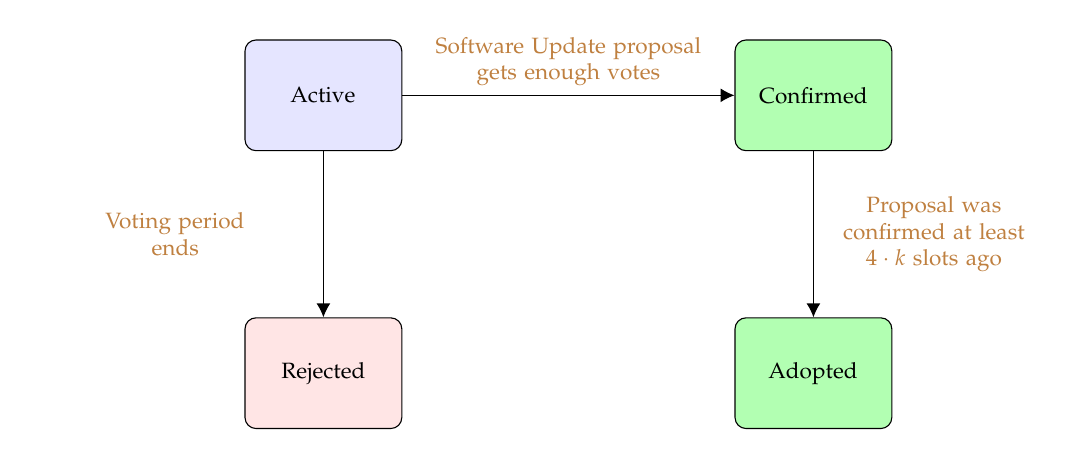
\begin{tikzpicture}[ align = center
                     , node distance = 6em and 12em
                     , text width = 5em
                     , font = \footnotesize
                     , >={Latex[width=0.5em, length=0.5em]}
                     , every node/.style = { rectangle
                                         , rounded corners
                                         , draw = black
                                         , align = center
                                         , minimum height = 4em }
                     ]

  \node (active) [fill = blue!10] {Active};
  \node (rejected) [below = of active, fill = red!10] {Rejected};
  \node (confirmed) [right = of active, fill = green!30] {Confirmed};
  \node (adopted) [below = of confirmed, fill = green!30] {Adopted};

  \tikzset{every node/.style={align=center, text width=10em, text=brown}}

  \draw[->] (active)
  edge node [above] {Software Update proposal\\ gets enough votes}
  (confirmed);

  \draw[->] (active)
  edge node [left] {Voting period \\ends}
  (rejected);

  \draw[->] (confirmed)
  edge node [right, text width=8em]
  {Proposal was confirmed at least $4 \cdot k$ slots ago}
  (adopted);


  \end{tikzpicture}

  \caption{State-transition diagram for software-updates}
  \label{fig:st-diagram-sw-up}
\end{figure}

\clearpage

A sequence of votes can be applied using $\trans{upivotes}{}$ transitions. The
inference rules for them are presented in \cref{fig:rules:apply-votes}. After
applying a sequence of votes, proposals might get confirmed, which means that
they will be added to the set $\var{cps'}$. In such case, the mapping of
application names to their latest version known to the ledger will be updated to
include the information about the confirmed proposals. Note that, unlike
protocol updates, software updates take effect as soon as a proposal is
confirmed (we cannot wait for stability since we need to preserve compatibility
with the existing chain, where there are software update proposals that were
adopted without waiting for $2\cdot k$ slots). In this rule, we also delete the
confirmed id's from the set of registered application update proposals
($\var{raus}$), since this information is no longer needed once the
application-name to software-version map ($\var{avs}$) is updated.

Also note that, unlike the rules of \cref{fig:rules:upi-ec}, we need not remove
other update proposals that refer to the software names whose versions were
changed in $\var{avs_{new}}$. The reason for this is that the range of $\var{raus}$
can contain only one pair of the form $(\var{an}, \wcard, \wcard)$ for any given
application name $\var{an}$ (see Rule~\ref{eq:rule:up-av-validity}).


\begin{figure}[htb]
  \begin{equation}
    \label{eq:rule:apply-votes-base}
    \inference
    {
    }
    {
      {\left(
        \begin{array}{l}
          s_n\\
          \var{dms}
        \end{array}
      \right)}
      \vdash
      \var{us}
      \trans{applyvotes}{\epsilon}
      \var{us}
    }
  \end{equation}
  %
  \nextdef
  %
  \begin{equation}
    \label{eq:rule:apply-votes-ind}
    \inference
    {
      {\left(
        \begin{array}{l}
          s_n\\
          \var{dms}
        \end{array}
      \right)}
      \vdash
      \var{us}
      \trans{applyvotes}{\Gamma}
      \var{us'}
      &
      {\left(
        \begin{array}{l}
          s_n\\
          \var{dms}
        \end{array}
      \right)}
      \vdash
      \var{us'}
      \trans{\hyperref[fig:rules:upi-vote]{upivote}}{v}
      \var{us''}
    }
    {
      {\left(
        \begin{array}{l}
          s_n\\
          \var{dms}
        \end{array}
      \right)}
      \vdash
      \var{us}
      \trans{applyvotes}{\Gamma;v}
      \var{us''}
    }
  \end{equation}
  %
  \nextdef
  %
  \begin{equation}
    \label{eq:rule:upivotes}
    \inference{
      {\left(
        \begin{array}{l}
          s_n\\
          \var{dms}
        \end{array}
      \right)}
      \vdash
      {\left(
          \begin{array}{l}
            (\var{pv}, \var{pps})\\
            \var{fads}\\
            \var{avs}\\
            \var{rpus}\\
            \var{raus}\\
            \var{cps}\\
            \var{vts}\\
            \var{bvs}\\
            \var{pws}
          \end{array}
        \right)}
      \trans{applyvotes}{\Gamma}
      {\left(
          \begin{array}{l}
            (\var{pv'}, \var{pps'})\\
            \var{fads'}\\
            \var{avs'}\\
            \var{rpus'}\\
            \var{raus'}\\
            \var{cps'}\\
            \var{vts'}\\
            \var{bvs'}\\
            \var{pws'}
          \end{array}
      \right)}\\
      %
      {\begin{array}{r@{~\leteq~}l}
        \var{cfm_{raus}} & \dom~(cps') \restrictdom \var{raus'}\\
        \var{avs_{new}} & \{ \var{an} \mapsto (\var{av}, \var{s_n}, m)
        \mid (\var{an}, \var{av}, m) \in \var{cfm_{raus}} \}
      \end{array}}
    }{
      {\left(
        \begin{array}{l}
          s_n\\
          \var{dms}
        \end{array}
      \right)}
      \vdash
      {\left(
          \begin{array}{l}
            (\var{pv}, \var{pps})\\
            \var{fads}\\
            \var{avs}\\
            \var{rpus}\\
            \var{raus}\\
            \var{cps}\\
            \var{vts}\\
            \var{bvs}\\
            \var{pws}
          \end{array}
      \right)}
      \trans{upivotes}{\Gamma}
      {\left(
          \begin{array}{l}
            (\var{pv'}, \var{pps'})\\
            \var{fads'}\\
            \var{avs'} \unionoverrideRight \var{avs_{new}}\\
            \var{rpus'}\\
            \dom~(cps') \subtractdom \var{raus'}\\
            \var{cps'}\\
            \var{vts'}\\
            \var{bvs'}\\
            \var{pws'}
          \end{array}
      \right)}
    }
  \end{equation}
  \caption{Applying multiple votes on update-proposals rules}
  \label{fig:rules:apply-votes}
\end{figure}
\clearpage

The interface rule for protocol-version endorsement makes use of the
$\trans{upend}{}$ transition, where we set the threshold for proposal adoption
to: the number of genesis keys ($\var{ngk}$) times the minimum proportion of
genesis keys that need to endorse an update proposal for it to become a
candidate for adoption (given by the protocol parameter $\var{upAdptThd}$). In
addition, the unconfirmed proposals that are older than $u$ blocks are removed
from the parts of the state that hold:
\begin{itemize}
\item the registered protocol and software update proposals,
\item the votes associated with the proposals,
\item the set of endorsement-key pairs, and
\item the block number in which proposals where added.
\end{itemize}

In Rule~\ref{eq:rule:upi-pend}, the set of proposal id's $\var{pid_{keep}}$
contains only those proposals that haven't expired yet or that are confirmed.
Once a proposal $\var{up}$ is confirmed, it is removed from the set of
confirmed proposals ($\var{cps}$) when a new a protocol version gets adopted
(see Rule~\ref{eq:rule:upi-ec-pv-change}).
%
The set of endorsement-key pairs is cleaned here as well as in the epoch change
rule (Rule~\ref{eq:rule:upi-ec-pv-change}). The reason for this is that this set grows at
each block, and it can get considerably large if no proposal gets adopted at
the end of an epoch.

\begin{figure}[htb]
  \begin{equation}
    \label{eq:rule:upi-pend}
    \inference
    {
      \var{upAdptThd} \mapsto q \in \var{pps} \\
      \left({
        \begin{array}{l}
          s_n\\
          \floor{q \cdot \var{ngk}}\\
          \var{dms}\\
          \var{cps}\\
          \var{rpus}
        \end{array}
      }\right)
      \vdash
      {
        \left(
          \begin{array}{l}
            \var{fads}\\
            \var{bvs}
          \end{array}
        \right)
      }
      \trans{\hyperref[fig:rules:up-end]{upend}}{(\var{bv}, \var{vk})}
      {
        \left(
          \begin{array}{l}
            \var{fads'}\\
            \var{bvs'}
          \end{array}
        \right)
      }\\
      \var{upropTTL} \mapsto u \in \var{pps}\\
      {
        \begin{array}{r@{~\leteq~}l}
          \var{pids_{keep}} & \dom~(pws \restrictrange [s_n - u, ..]) \cup \dom~\var{cps}\\
          \var{vs_{keep}} & \dom~(\range~\var{rpus'})\\
          \var{rpus'} & \var{pids_{keep}} \restrictdom \var{rpus}
        \end{array}
      }
    }
    {
      {\left(
        \begin{array}{l}
          s_n\\
          \var{dms}
        \end{array}
      \right)}
      \vdash
      {
        \left(
          \begin{array}{l}
            (\var{pv}, \var{pps})\\
            \var{fads}\\
            \var{avs}\\
            \var{rpus}\\
            \var{raus}\\
            \var{cps}\\
            \var{vts}\\
            \var{bvs}\\
            \var{pws}
          \end{array}
        \right)
      }
      \trans{upiend}{(\var{bv}, \var{vk})}
      {
        \left(
          \begin{array}{l}
            (\var{pv}, \var{pps})\\
            \var{fads'}\\
            \var{avs}\\
            \var{rpus'}\\
            \var{pids_{keep}} \restrictdom \var{raus}\\
            \var{cps}\\
            \var{pids_{keep}} \restrictdom \var{vts}\\
            \var{vs_{keep}}  \restrictdom \var{bvs'}\\
            \var{pids_{keep}} \restrictdom \var{pws}
          \end{array}
        \right)
      }
    }
  \end{equation}
  \caption{Proposal endorsement rules}
  \label{fig:rules:upi-pend}
\end{figure}

\clearpage

Rule~\ref{eq:rule:upi-ec-pv-change} models how the protocol-version and its
parameters are changed depending on an epoch change signal.
%
On an epoch change, this rule will pick a candidate that gathered enough
endorsements at least $4 \cdot k$ slots ago. If a protocol-version candidate
cannot gather enough endorsements $4 \cdot k$ slots before the end of an epoch,
the proposal can only be adopted in the next epoch. The reason for the $4 \cdot
k$ slot delay is to allow a period between knowing when a proposal will be
adopted, and the event of its being adopted. Since update proposals can and will
make large changes to the way the chain operates, it is useful to be able to
guarantee a window in which it is known that no update will take place.
%
Figure~\ref{fig:up-confirmed-too-late} shows an example of a proposal being
confirmed too late in an epoch, where it is not possible to get enough
endorsements in the remaining window. In this Figure we take $k = 2$, and we
assume $4$ endorsements are needed to consider a proposal as candidate for
adoption.
%
Note that, in the final state, we use union override to define the updated
parameters ($\var{pps} \unionoverrideRight \var{pps'}$). This is because candidate
proposal might only update some parameters of the protocol.

In Rule~\ref{eq:rule:upi-ec-pv-change}, when a new proposal gets adopted, all
the state components that refer to protocol update proposals get emptied. The
reason for this is that at the moment of registering a proposal, we evaluated
it in a state where the protocol parameters that we used for this are no longer
up to date (see for instance \cref{eq:func:can-update}). For instance, assume
we register a proposal $\var{up}$ which only changes the maximum transaction
size to $x$, and the current block size is set to $x + 1$. Then,
$\fun{canUpdate}$ holds, since the maximum transaction size is less than the
maximum block size. If now a new proposal gets adopted that changes the maximum
block size to $x - 1$, then this invalidates $\var{up}$ since $\fun{canUpdate}$
no longer holds.
%

If there are no candidates for adoption, then the state variables remain
unaltered (Rule~\ref{eq:rule:upi-ec-pv-unchanged}).

Also note that the registered software-update proposals need not be cleaned
here, since this is done either when a proposal gets confirmed or when it
expires.

\begin{figure}[htb]
  \begin{equation}
    \label{eq:rule:pvbump-change-epoch-only}
    \inference
    {
      [.., s_n - 4 \cdot k] \restrictdom \var{fads} = \epsilon
    }
    {
      {\left(\begin{array}{l}
         s_n\\
         \var{fads}
       \end{array}\right)}
      \vdash
      {
        \left(
          \begin{array}{l}
            \var{pv}, \var{pps}\\
          \end{array}
        \right)
      }
      \trans{pvbump}{}
      {
        \left(
          \begin{array}{l}
            \var{pv}, \var{pps}\\
          \end{array}
        \right)
      }
    }
  \end{equation}
  \nextdef
  \begin{equation}
    \label{eq:rule:pvbump-change}
    \inference
    {
      \wcard ; (\wcard , (\var{pv_c}, \var{pps_c})) \leteq [.., s_n - 4 \cdot k] \restrictdom \var{fads}
    }
    {
      {\left(\begin{array}{l}
         s_n\\
         \var{fads}
       \end{array}\right)}
      \vdash
      {
        \left(
          \begin{array}{l}
            \var{pv}, \var{pps}\\
          \end{array}
        \right)
      }
      \trans{pvbump}{}
      {
        \left(
          \begin{array}{l}
            \var{pv_c}, \var{pps_c}\\
          \end{array}
        \right)
      }
    }
  \end{equation}
  \caption{Protocol version bump rules}
  \label{fig:rules:pvbump}
\end{figure}

\begin{figure}[htb]
  \begin{equation}
    \label{eq:rule:upi-ec-pv-unchanged}
    \inference
    {
      {\left(\begin{array}{l}
         \fun{firstSlot}~e_n\\
         \var{fads}
       \end{array}\right)}
      \vdash
      {
        \left(
          \begin{array}{l}
            \var{pv}, \var{pps}
          \end{array}
        \right)
      }
      \trans{\hyperref[fig:rules:pvbump]{pvbump}}{}
      {
        \left(
          \begin{array}{l}
            \var{pv'}, \var{pps'}\\
          \end{array}
        \right)
      } &\var{pv} = \var{pv'}
    }
    {
      (e_n)
      \vdash
      {
        \left(
          \begin{array}{l}
            (\var{pv}, \var{pps})\\
            \var{fads}\\
            \var{avs}\\
            \var{rpus}\\
            \var{raus}\\
            \var{cps}\\
            \var{vts}\\
            \var{bvs}\\
            \var{pws}
          \end{array}
        \right)
      }
      \trans{upiec}{}
      {
        \left(
          \begin{array}{l}
            (\var{pv}, \var{pps})\\
            \var{fads}\\
            \var{avs}\\
            \var{rpus}\\
            \var{raus}\\
            \var{cps}\\
            \var{vts}\\
            \var{bvs}\\
            \var{pws}
          \end{array}
        \right)
      }
    }
  \end{equation}
  \nextdef
  \begin{equation}
    \label{eq:rule:upi-ec-pv-change}
    \inference
    {
      {\left(\begin{array}{l}
         \fun{firstSlot}~e_n\\
         \var{fads}
       \end{array}\right)}
      \vdash
      {
        \left(
          \begin{array}{l}
            \var{pv}, \var{pps}\\
          \end{array}
        \right)
      }
      \trans{\hyperref[fig:rules:pvbump]{pvbump}}{}
      {
        \left(
          \begin{array}{l}
            \var{pv'}, \var{pps'}\\
          \end{array}
        \right)
      }
      & \var{pv} \neq \var{pv'}
    }
    {
      (e_n)
      \vdash
      {
        \left(
          \begin{array}{l}
            \var{(\var{pv}, \var{pps})}\\
            \var{fads}\\
            \var{avs}\\
            \var{rpus}\\
            \var{raus}\\
            \var{cps}\\
            \var{vts}\\
            \var{bvs}\\
            \var{pws}
          \end{array}
        \right)
      }
      \trans{upiec}{}
      {
        \left(
          \begin{array}{l}
            (\var{pv'}, \var{pps'})\\
            \epsilon\\
            \var{avs}\\
            \emptyset\\
            \emptyset\\
            \emptyset\\
            \emptyset\\
            \emptyset\\
            \emptyset\\
          \end{array}
        \right)
      }
    }
  \end{equation}
  \caption{Block version adoption on epoch change rules}
  \label{fig:rules:upi-ec}
\end{figure}

\begin{figure}[htb]
  \centering
  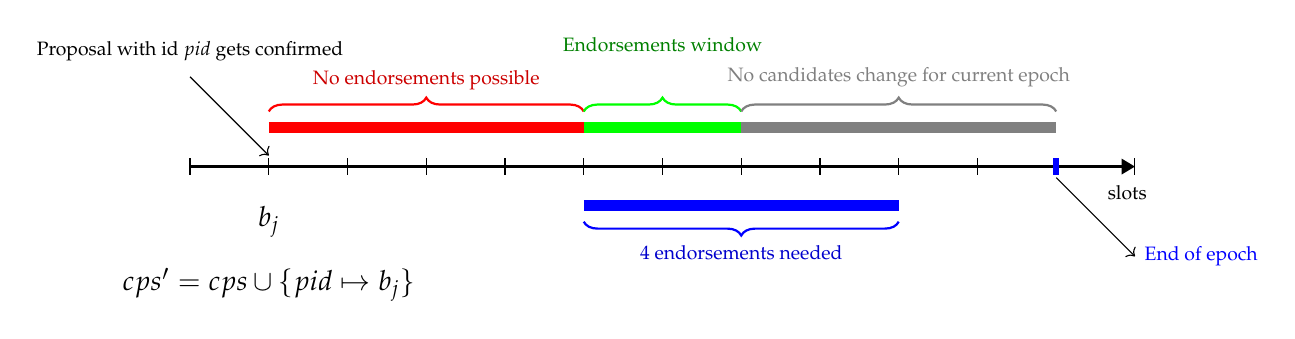
\begin{tikzpicture}
    %%
    %% Macros used in this picture
    %%
    %
    % Number of slots
    \pgfmathsetmacro{\nrSlots}{12}
    % Slot in which the proposal gets confirmed
    \pgfmathsetmacro{\cSlot}{1}
    % Our special K.
    \pgfmathsetmacro{\K}{4}
    % Epoch end.
    \pgfmathsetmacro{\eend}{11}
    % Number of positive votes needed
    \pgfmathsetmacro{\votes}{4}

    % Draw the horizontal line
    \draw[thick, -Triangle] (0,0) -- (\nrSlots,0)
    node[font=\scriptsize,below left=3pt and -8pt]{slots};

    % % draw vertical lines
    \foreach \x in {0,1,...,\nrSlots}
    \draw (\x cm, 3pt) -- (\x cm, -3pt);

    % Add a label to with the block number in which the proposal got confirmed.
    \node at (\cSlot, -.7) {$b_j$};

    % Update in cps
    \node at (\cSlot, -1.5) {$\var{cps'} = \var{cps} \cup \{ \var{pid} \mapsto b_j \}$};

    % The no-endorsements red bar.
    \draw[red, line width=4pt] (\cSlot, .5) -- +(\K, 0);

    % Brace above the no-endorsement window bar.
    \draw[thick, red, decorate, decoration={brace, amplitude=5pt}]
    (\cSlot, .7) -- +(\K, 0)
    node[black!20!red, midway, above=4pt, font=\scriptsize] {No endorsements possible};

    % The endorsements window.
    \coordinate (ewStart) at (\cSlot + \K, .5);
    \coordinate (ewEnd) at ($(\eend - \K, .5)$);
    \draw[green, line width=4pt]
    (ewStart) -- (ewEnd);

    % Brace above the endorsements window
    \coordinate (ewStartB) at ($(ewStart) + (0, 0.2)$);
    \coordinate (ewEndB) at ($(ewEnd) + (0, 0.2)$);
    \draw[thick, green, decorate, decoration={brace, amplitude=5pt}]
    (ewStartB) -- (ewEndB)
    node[black!50!green, midway, above=18pt, font=\scriptsize] {Endorsements window};

    % The no-candidates change window.
    \coordinate (nccStart) at (\eend - \K, .5);
    \coordinate (nccEnd) at ($(\eend, .5)$);
    \draw[gray, line width=4pt]
    (nccStart) -- (nccEnd);

    % Brace above the no-candidates change window.
    \coordinate (nccStartB) at ($(nccStart) + (0, 0.2)$);
    \coordinate (nccEndB) at ($(nccEnd) + (0, 0.2)$);
    \draw[thick, gray, decorate, decoration={brace, amplitude=5pt}]
    (nccStartB) -- (nccEndB)
    node[gray, midway, above=5pt, font=\scriptsize] {No candidates change for current epoch};


    % The 2k before end-of-epoch window.
    \coordinate (beeStart) at (\cSlot + \K, -.5);
    \coordinate (beeEnd) at ($(\cSlot + \K + \votes, -.5)$);
    \draw[blue, line width=4pt]
    (beeStart) -- (beeEnd);

    % Brace on above the 2k before end-of-epoch window.
    \coordinate (beeStartB) at ($(beeStart) - (0, 0.2)$);
    \coordinate (beeEndB) at ($(beeEnd) - (0, 0.2)$);
    \draw[thick, blue, decorate, decoration={brace, amplitude=5pt}]
    (beeEndB) -- (beeStartB)
    node[black!20!blue, midway, below=5pt, font=\scriptsize] {$\votes$ endorsements needed};

    \draw[blue, line width=2pt] (\eend, 3pt) -- (\eend, -3pt);

    \draw[<-] (\cSlot, 4pt) -- +(-1, 1)
    node [above=2pt, black, font=\scriptsize]
    {Proposal with id $\var{pid}$ gets confirmed};

    \draw[->] (\eend, -4pt) -- +(1, -1)
    node[right, blue, font=\scriptsize] {End of epoch};
  \end{tikzpicture}
  \caption{An update proposal confirmed too late}
  \label{fig:up-confirmed-too-late}
\end{figure}

Figure~\ref{fig:st-diagram-pt-up} shows the different states a protocol-update
proposal can be in, and what causes the transitions between them.

\begin{figure}[ht]
  \centering
  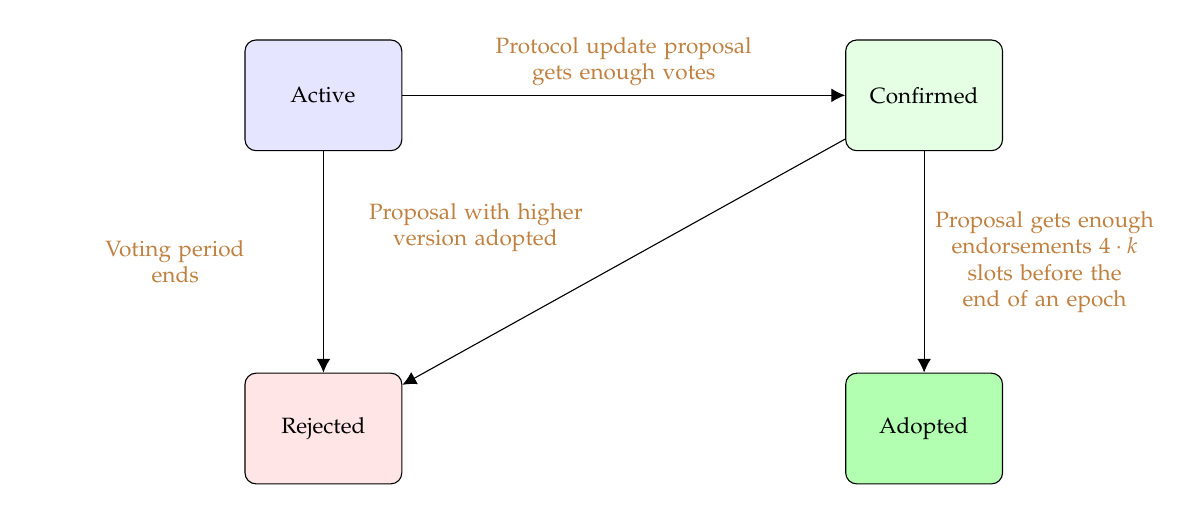
\begin{tikzpicture}[ align = center
                     , node distance = 8em and 16em
                     , text width = 5em
                     , font = \footnotesize
                     , >={Latex[width=0.5em, length=0.5em]}
                     , every node/.style = { rectangle
                                         , rounded corners
                                         , draw = black
                                         , align = center
                                         , minimum height = 4em }
                     ]

  \node (active) [fill = blue!10] {Active};
  \node (rejected) [below = of active, fill = red!10] {Rejected};
  \node (confirmed) [right = of active, fill = green!10] {Confirmed};
  \node (adopted) [below = of confirmed, fill = green!30] {Adopted};

  \tikzset{every node/.style={align=center, text width=10em, text=brown}}

  \draw[->] (active)
  edge node [above] {Protocol update proposal\\ gets enough votes}
  (confirmed);

  \draw[->] (active)
  edge node [left] {Voting period \\ends}
  (rejected);

  \draw[->] (confirmed)
  edge node [above left]
  {Proposal with higher version adopted}
  (rejected);

  \draw[->] (confirmed)
  edge node [right, text width=8em]
  {Proposal gets enough endorsements $4 \cdot k$ slots before the end of an epoch}
  (adopted);

  \end{tikzpicture}

  \caption{State-transition diagram for protocol-updates}
  \label{fig:st-diagram-pt-up}
\end{figure}


\section{Formal Properties}
\label{sec:properties}

This appendix collects the main formal properties that the new ledger rules are expected to satisfy.
Note here that in every property in this section we consider a only phase-1 valid
transactions, ie. ones that can indeed get processed.

\begin{enumerate}[label=P{\arabic*}:\ ]
\item
  \emph{Consistency with Shelley.}
  \begin{itemize}
    \item properties 15.6 - 15.16 (except 15.8 and 15.13) hold specifically in the $\fun{txValTag}~tx~=~\True$ case, because
    the calculations refer to the UTxO as if it was updated by a scripts-validating transaction
    \item other properties hold as-is
  \end{itemize}

\item
  \emph{Consistency with Multi-Asset.}
  \begin{itemize}
    \item properties 8.1 and 8.2 hold specifically in the $\fun{txValTag}~tx~=~\True$ case, because
    the calculations refer to the UTxO as if it was updated by a scripts-validating transaction
    \item other properties hold as-is
  \end{itemize}
\end{enumerate}


\begin{definition}
  For a state $s$ that is used in any subtransaction of
  $\mathsf{CHAIN}$, we define $\Utxo(s) \in \UTxO$ to be the $\UTxO$
  contained in $s$, or an empty map if it does not exist. This is
  similar to the definition of $\Val$ in the Shelley specification.

  Similarly, we also define $\field_{v}~(s)$ for the field $v$ that is part of
  the ledger state $s$, referenced by the typical variable name (eg. $\var{fees}$
  for the fee pot on the ledger).
\end{definition}

We also define a helper function $\varphi$ as follows:
\[\varphi(x, tx) :=
  \begin{cases}
    x & \fun{txValTag}~tx = \True \\
    0 & \fun{txValTag}~tx = \False
  \end{cases}\]
This function is useful to distinguish between the two
cases where a transaction can mint tokens or not, depending on whether
its scripts validate.

\begin{property}[General Accounting]
  \label{prop:pov}
  The \emph{general accounting} property in Alonzo encompasses two parts
  \begin{itemize}
    \item preservation of value property expressed via the $\fun{produced}$ and $\fun{consumed}$
    calculations, applicable for transactions with $\fun{txValTag}~tx~=~\True$, which
    is specified as in the ShelleyMA POV.
    \item the preservation of value for $\fun{txValTag}~tx~=~\False$, when
    only the collateral fees are collected into the fee pot.
  \end{itemize}

Both of these are expressed in the following lemma.

\begin{lemma}
  For all environments $e$, transactions $tx$ and states $s, s'$, if
  \begin{equation*}
    e\vdash s\trans{utxos}{tx}s'
  \end{equation*}
  then
  \begin{equation*}
    \Val(s) + \varphi(\fun{mint}~(\fun{txbody}~tx), tx) = \Val(s')
  \end{equation*}
\end{lemma}

\begin{proof}
  In the case that $\fun{txValTag}~tx = \True$ holds, the proof is
  identical to the proof of Lemma 9.1 of the multi-asset
  specification. Otherwise, the transition must have been done via the
  $\mathsf{Scripts-No}$ rule, which removes
  $\fun{collateral}~(\fun{txbody}~tx)$ from the UTxO, and increases the fee pot by the amount of the sum of Ada in the
  collateral UTxO entries. The value contained in $s$ is not changed.

  Note that in the $\fun{feesOK}$ function, there is a check that verifies
  that, in the case that there are phase-2 scripts, there are no non-Ada tokens in the UTxOs
  which the collateral inputs reference, so non-Ada tokens do not get minted, burned, or transferred
  in this case.
\end{proof}
\end{property}

\begin{property}[Extended UTxO Validation]
  \label{prop:fees-only}

  If a phase-1 valid transaction extends the UTxO, all its scripts validate
  (i.e. $\fun{txValTag}~tx = \True$).

  If a transaction is accepted and marked as paying collateral only
  (i.e. $\fun{txValTag}~tx = \False$), then the only change to the ledger
  when processing the transaction is that the collateral inputs
  are moved to the fee pot. In particular, it does not extend the UTxO.

  \begin{lemma}
    For all environments $e$, transactions $tx$ and states $s, s'$, if  and
    \begin{equation*}
      e\vdash s\trans{ledger}{tx}s'
    \end{equation*}
    then
    \[\Utxo(s') \nsubseteq \Utxo(s)~\Rightarrow~\fun{txValTag}~tx = \True \]

    Also,
    \[\fun{txvaltag}~tx = \False~ \Rightarrow~\]
    \begin{itemize}
      \item $ \field_{v}~(s') = \field_{v}~(s) \text{ for all } v~\neq~{fees}, ~v~\neq~{utxo}$
      \item $\field_{fees}~(s') = \field~\var{fees}~(s) + \fun{coin}~(\Val~(\fun{collateral}~{tx} \subtractdom \Utxo(s)))$
      \item $\Utxo(s') = \fun{collateral}~{tx} \subtractdom \Utxo(s)$
    \end{itemize}
  \end{lemma}

  \begin{proof}
    A ledger UTxO update is specified explicitly only by the $\mathsf{UTXOS}$ transition,
    and propagated (ie. applied as-specified) to a chain-state update via the
    $\mathsf{UTXO}$ and $\mathsf{UTXOW}$ transitions.

    The only case in which the $\mathsf{UTXOS}$ transition adds entries to the UTxO
    map is in the $\mathsf{Scripts-No}$ rule, when $\fun{txValTag}~tx = \True$.
    Adding entries to the UTxO map implies exactly that the updated map is not a
    submap of the original, so we get that

    \[\Utxo(s') \nsubseteq \Utxo(s)~\Rightarrow~\fun{txValTag}~tx = \True \]

   In the case that $\fun{txValTag}~tx = \False$, $\mathsf{LEDGER}$ calls the rule
   that does not update $\DPState$ at all, only the $\UTxOState$. This state update is specified
   in the $\mathsf{UTXOS}$ transition (and applied via the $\mathsf{UTXO}$ and $\mathsf{UTXOW}$ transitions).

   The only parts of the state that are updated are
   \begin{itemize}
     \item the fee pot, which is increased by the amount of the sum of Ada in the
     collateral UTxO entries, and
     \item the UTxO, where the collateral entries
     are removed.
   \end{itemize}
  \end{proof}
\end {property}

\begin{property}[Validating when No NN Scripts]
  \label{prop:is-valid}

Whenever a valid transaction does not have any phase-2 scripts, its
$\fun{txValTag} = \True$.

\begin{lemma}
  For all environments $e$, transactions $tx$ and states $s, s'$ such that
  \begin{equation*}
    e\vdash s\trans{ledger}{tx}s',
  \end{equation*}
  If $\range (\fun{txscripts}~tx) \cap \ScriptPhTwo = \emptyset$
  then $\fun{txValTag} = \True$.
\end{lemma}
\begin{proof}
  With the same argument as previously, we only need to discuss the
  equivalent claim for the $\mathsf{UTXOS}$ transition. Under these
  assumptions, $\var{sLst} := \fun{collectTwoPhaseScriptInputs}$ is an empty
  list. Thus $\fun{evalScripts}~sLst = \True$, and the transition rule
  had to be $\mathsf{Scripts{-}Yes}$.
\end{proof}
\end{property}

\begin{property}[Paying fees]
  \label{prop:pay-fees}

In the case that all phase-2 scripts in a transaction validate, the transaction pays
at least the minimum transaction fee amount into the fee pot. In the case that
some do not validate, it must pay at least the percentage of the minimum fee
the collateral is required to cover.

\begin{lemma}
  For all environments $e$, transactions $tx$ and states $s, s'$ such that
  \begin{equation*}
    e\vdash s\trans{ledger}{tx}s'
  \end{equation*}
  The following holds : \\
  $\field_{fees}~(s')~\geq~\field_{fees}~(s)~+
  \begin{cases}
    \fun{minfee}~{tx} & \fun{txValTag} = \True \\
    \fun{quot}~(\fun{collateralPercent}~(\field_{pp}~(s)))~*~(\fun{minfee}~{tx})~100 & \fun{txValTag} = \False\\
  \end{cases}$.
\end{lemma}
\begin{proof}
  The fee pot is updated by the $\mathsf{Scripts{-}Yes}$ and the $\mathsf{Scripts{-}No}$
  rules, one of which is necessarily called by a valid transaction via the sequence
  of transitions called in the order $\mathsf{LEDGER}, \mathsf{UTXOW}, \mathsf{UTXO}, \mathsf{UTXOS}$.

  The $\mathsf{Scripts{-}Yes}$ rule (i.e. $\fun{txValTag} = \True$)
  transfers the amount of Lovelace in the $\fun{txfee}$ field of the
  transaction to the fee pot, which is checked to be at least the $\fun{minfee}$
  by $\fun{feesOK}$ in the $\mathsf{UTXO}$ transition. So, we get

  \[\field_{fees}~(s')~=~\field_{fees}~(s)~+~\fun{txfee}~{tx}~\geq~\field_{fees}~(s)~+~\fun{minfee}~{tx}\]

  The $\mathsf{Scripts{-}No}$ rule (i.e. $\fun{txValTag} = \False$) removes the
  $\fun{collateral}$ inputs from the
  UTxO, and adds the balance of these realized inputs to the fee pot.

  \[\field_{fees}~(s')~=~field_{fees}~(s)~+~\fun{ubalance}~(\fun{collateral}~{txb} \restrictdom \var{utxo})\]

  We can conclude that $\fun{txrdmrs}$ is non-empty whenever $\fun{txValTag} = \False$
  from the following observations :
  \begin{itemize}
    \item $\fun{txValTag} = \False$ whenever $\fun{evalScripts}$ fails.
    \item $\fun{evalScripts}$ is a $\wedge$-fold over a list of scripts and
    their inputs, containing all scripts that need to be run to validate this transaction
    \item All phase-1 scripts must succeed, as this is checked in phase-1 validation (UTXOW
    rule check). Therefore,
    $\fun{evalScripts}$ encounters a failing script which is phase-2.
    \item All phase-2 scripts necessarily have an associated redeemer attached to the
    transaction (UTXOW rule check)
  \end{itemize}

  See Property~\ref{prop:fixed-inputs} for more details on what inputs $\fun{evalScripts}$ has,
  and what we can say about the outcome of its computation with respect to its inputs.

  The $\fun{feesOK}$ check enforces that if a transaction has a non-empty
  $\fun{txrdmrs}$ field, the balance of the realized collateral inputs
  (which $\field_{fees}~(s)$ is increased by as part of processing $tx$) is

  \[\fun{ubalance}~(\fun{collateral}~{txb} \restrictdom \var{utxo})~\geq~\fun{quot}~(\txfee~{txb} * (\fun{collateralPercent}~pp))~100\]

  which, since $\txfee~{txb}~\geq~\fun{minfee}~{txb}$, gives

  \[ \geq~\fun{quot}~(\fun{minfee}~{txb} * (\fun{collateralPercent}~pp))~100)) \]

  where $\fun{txbody}~{tx}~=~{txb}$. This shows that the total collateral that gets
  moved into the fee pot from the UTxO by the $\mathsf{Scripts{-}No}$ rule is at
  least the minimum transaction fee scaled by the collateral percent parameter.

  \[\field_{fees}~(s')~\geq~\field_{fees}~(s)~+~\fun{quot}~(\fun{minfee}~{txb} * (\fun{collateralPercent}~pp))~100))\]
\end{proof}

An immediate corollary to this property is that when the $\fun{collateralPercent}$ is set to 100 or more,
the transaction always pays at least the minimum fee. This, in turn, implies that it
pays at least the fee that it has stated in the $\fun{txfee}$ field.

\begin{corollary}
  For all environments $e$, transactions $tx$ and states $s, s'$ such that
  \begin{equation*}
    e\vdash s\trans{ledger}{tx}s'~~\wedge~~\fun{collateralPercent}~(\field_{pp}~(s)) \geq 100
  \end{equation*}
  The following holds :
  \[\field_{fees}~(s')~\geq~\field_{fees}~(s)~+~\fun{minfee}~{tx} \]
\end{corollary}

\begin{proof}
  In both two cases in the lemma above, the $\field_{fees}$ field in the ledger state
  is increased by at least $\fun{minfee}~{tx}$ :
  \begin{itemize}
    \item when $\fun{txValTag} = \True$, the lemma states already that
    \[\field_{fees}~(s')~\geq~\field_{fees}~(s)~+~\fun{minfee}~{tx}\]
    \item when $\fun{txValTag} = \False$, we have
    $ \field_{fees}~(s')~\geq~\field_{fees}~(s)~+~\fun{quot}~(\fun{minfee}~{txb} * (\fun{collateralPercent}~pp))~100$ \\
    $~~~\geq~\field_{fees}~(s)~+~\fun{quot}~(\fun{minfee}~{tx}~*~100)~100$ \\
    $~~~=~\field_{fees}~(s)~+~\fun{minfee}~{tx}$
  \end{itemize}
\end{proof}

\end{property}

\begin{property}[Correct tag]
  \label{prop:correct-tag}

The $\fun{txValTag}~tx$ tag of a phase-1 valid transaction must match the result of the $\fun{evalScripts}$
function for that transaction.

\begin{lemma}
  For all environments $e$, transactions $tx$ and states $s, s'$ such that
  \begin{equation*}
    e\vdash s\trans{utxos}{tx}s',
  \end{equation*}
  The following holds :
    \[\fun{txValTag}~tx ~=~ \fun{evalScripts}~{tx}~{sLst} \]
  where
  \[ \var{sLst} \leteq \fun{collectTwoPhaseScriptInputs} ~\field_{pp}(s)~\var{tx}~ \Utxo(s) \]
\end{lemma}
\begin{proof}
  Inspecting the $\mathsf{Scripts{-}Yes}$ and the $\mathsf{Scripts{-}No}$ rules of the $\mathsf{UTXOS}$ transition,
  we see that both the $\fun{txValTag}$ and the result of $\fun{evalScripts}$
  are $\True$ in the former, and $\False$ in the latter.
\end{proof}
\end{property}

\begin{property}[Replay protection]
  \label{prop:replay}

A transaction always removes at least one UTxO entry from the ledger, which provides
replay protection.

\begin{lemma}
  For all environments $e$, transactions $tx$ and states $s, s'$ such that
  \begin{equation*}
    e\vdash s\trans{ledger}{tx}s',
  \end{equation*}
  The following holds : $\Utxo~(s)~\nsubseteq~\Utxo~(s')$.
\end{lemma}
\begin{proof}
  The UTxO is updated by the $\mathsf{Scripts{-}Yes}$ and the $\mathsf{Scripts{-}No}$
  rules, on of which is necessarily called by a valid transaction. Both of these
  rules remove UTxOs corresponding to a set of inputs.

  In both cases, there is a check that the removed inputs set is non-empty.
  The $\mathsf{Scripts{-}Yes}$ rule of the $\mathsf{UTXOS}$ transition
  removes the UTxOs associated with the input set $\fun{txinputs}~{tx}$ from the ledger.
  The $\fun{txinputs}~{tx}$ set must be non-empty because there is a check in the
  $\mathsf{UTXO}$ rule (which calls $\mathsf{UTXOS}$) that ensure this is true.

  For the $\mathsf{Scripts{-}No}$ rule of the $\mathsf{UTXOS}$ transition
  removes the UTxOs associated with the input set $\fun{collateral}~{tx}$ from the ledger.
  The $\fun{collateral}~{tx}$ set must be non-empty because
  the $\fun{feesOK}$ function (called by the same rule that calls $\mathsf{UTXO},
  \mathsf{UTXOS}$) ensures that in the case that the $tx$ contains phase-2 scripts,
  $\fun{collateral}~{tx}$ must be non-empty.

  Note that by property~\ref{prop:is-valid}, phase-2 scripts must always be present
  if $\fun{txValTag}~tx = \False$ (that is, whenever $\mathsf{Scripts{-}No}$ rule is used).
\end{proof}
\end{property}

\begin{property}[UTxO-changing transitions]
  \label{prop:utxo-change}

The $\mathsf{UTXOS}$ transition fully specifies the change in the ledger $\UTxO$
for each transaction.

\begin{lemma}
  For all environments $e$, transitions $\mathsf{TRNS}$, transactions $tx$ and states $s, s'$ such that
  \begin{equation*}
    e\vdash s\trans{trns}{tx}s'
  \end{equation*}
  The following holds :
  \begin{equation*}
    \Utxo(s) \neq \Utxo(s')~\Rightarrow~e'\vdash u\trans{utxos}{tx}u'
  \end{equation*}
  where $\Utxo(s) = \Utxo(u)~\wedge~\Utxo(s') = \Utxo(u')$ for some environment $e'$,
  and states $u, u'$.
\end{lemma}
\begin{proof}
  By inspecting each transition in this specification, as well as those inherited from the
    Shelley one, we see that a non-trivial update from the UTxO of $s$ to that of $s'$
    must be done by $\mathsf{UTXOS}$. Every other transition that changes the UTxO and
    has a signal of type $\Tx$ only applies the $\mathsf{UTXOS}$.
\end{proof}
\end{property}

\begin{property}[Script interpreter arguments are fixed (deterministic script evaluation)]
  \label{prop:fixed-inputs}

For this property, we make some assumptions about things that are outside the scope of this specifications :

\begin{itemize}
  \item The Plutus script
  interpreter is a pure function that receives only the arguments provided by the ledger when it is
  invoked by calling the $\fun{runPLCScript}$ function. We assume that this is
  also true in an implementation. In particular, the interpreter does not
  obtain any system randomness, etc.

  \item We assume that constructing the validation context from $\TxInfo$ and
  the $\ScriptPurpose$ by $\fun{valContext}$ is deterministic.

  \item We do not need to check here that the hashes that are the keys of the
  $\fun{txscripts}$ and $\fun{txdats}$ fields match the computed hashes of the scripts and
  datum objects they index. This is because these hashes must be computed as part of
  the deserialization of a transaction (see the CDDL specification),
  instead of being transmitted as part of the transaction and then checked. We
  assume these hashes are correct.

  \item We assume that the consensus
  function $\fun{epochInfoSlotToUTCTime}$ for converting a slot interval into a
  system time interval is deterministic.

  \item We assume that the two global
  constants, $\EpochInfo$ and $\SystemStart$, which it also takes as parameters,
  cannot change within the span of any interval for which $\fun{epochInfoSlotToUTCTime}$
  is able to convert both endpoints to system time.
\end{itemize}

The assumptions above are implicit in the functional style of definitions in this
specification, but they are worth pointing out for implementation.
With these assumptions in mind, we can say that
script evaluation is deterministic.

We split this result into a lemma and its corollary :

\begin{itemize}
  \item First, we demonstrate that all the scripts and their arguments that are
  collected for phase-2 validation are the same for two phase-1 valid transactions with the same body,
  independent of the (necessarily valid) ledger state to which they are being applied

  \item Second, we derive the corollary that under the same validity assumptions,
  phase-2 validation results in the same outcome for both transactions
\end{itemize}

\begin{lemma}
  \label{lem:inputs}
  For all environments $e, e'$, transactions $tx, tx'$ and states $s, s', u, u'$ such that
  $e$ and $s$ are subsets of fields of some valid chain state $c$, and
  $e'$ and $s'$ are subsets of fields of some valid chain state $c'$,

  \begin{equation*}
    e\vdash s\trans{ledger}{tx}s', \\
    e'\vdash u\trans{ledger}{tx'}u', \\
    \txbody{tx} = \txbody{tx'}
  \end{equation*}

  The following holds :

  \[\fun{toSet}~(\fun{collectTwoPhaseScriptInputs} ~\field_{pp}(s)~\var{tx}~ \Utxo(s))\]
  \[ = \]
  \[\fun{toSet}~(\fun{collectTwoPhaseScriptInputs} ~\field_{pp}(u)~\var{tx'}~ \Utxo(u))\]

\end{lemma}
\begin{proof}

    The $\fun{collectTwoPhaseScriptInputs}$
    function (see \ref{fig:functions:script2})
    constructs a list where each entry contains a Plutus script
    and the arguments passed to the interpreter for its evaluation.

    To show that $\fun{collectTwoPhaseScriptInputs}$ returns a list containing
    the same elements for both $tx$ and $tx'$, we observe that
    the set of elements from which this list is produced via $\fun{toList}$
    is generated using the following functions, as well as set comprehension
    and list operations.
    We demonstrate that the functions used in this definition
    produce the same output for $tx$ and $tx'$, as all the data they
    inspect is fixed by the transaction body :

    \begin{itemize}
      \item $\fun{scriptsNeeded}$ : The $\PolicyID$, $\AddrRWD$, and $\DCert$ data
      output by this function as the second term of the hash-purpose pair
      is obtained directly from the $\fun{mint}$, $\fun{txwdrls}$,
      $\fun{txcerts}$ fields of the transaction, which are all fixed by the
      body of the transaction. These types of script purposes all include
      the hash of the validating script.

      The only other data this function inspects is the UTxO entries associated
      with the $\fun{txinputs}$ (passed via the $\UTxO$ argument) to get the realized inputs.
      We know that the UTxO is a field in a valid chain state for both the phase-1 valid
      transactions $tx$ and
      the $tx'$ ($\Utxo(s)$ and $\Utxo(u)$, respectively). This means that the $\TxId$
      in each input present in either UTxO is a hash of the body of the transaction
      containing the $\TxOut$ part of the UTxO entry indexed by that input. The
      order of the outputs is also fixed by the body, which fixes the $\Ix$ of
      the entry.

      A different value in output part of the UTxO entry (or a different order of
      outputs) would necessarily imply
      that the hash of the body containing that output must be different.
      Therefore, for all Plutus script-locked realized inputs of either transaction,
      the script hash in the payment credential of the address
      (and, by the same argument, the datum hash) are fixed by the inputs in body of the
      transaction, despite not being explicitly contained in it. We then get that

      \[ \fun{scriptsNeeded}~\Utxo(s)~(\txbody{tx}) = \fun{scriptsNeeded}~\Utxo(u)~(\txbody{tx'}) \]

      \item $\fun{getDatum}$ : In the case the script purpose
      is of the input type, the datum this function returns is one that
      is associated with the corresponding realized input. More precisely, it is the datum whose
      hash is specified in the realized input, and is looked up by hash in the $\fun{txdats}$
      transaction field. If there is no datum hash in the realized input, or the script purpose
      is of a non-input type, the empty list is returned.

      The $\mathsf{UTXOW}$ rule checks that the transaction is carrying all datums corresponding
      to its realized inputs. Since the inputs (and realized inputs) are the same
      for $tx$ and $tx'$ (fixed by the body), this guarantees that
      of the datum hashes in the realized inputs (and therefore, their preimages)
      are the same as well.

      \item $\fun{txscripts}$ : in the $\mathsf{UTXOW}$ rule, there is a check that all the
      script preimages of the script hashes returned by the $\fun{scriptsNeeded}$
      function must be present in this field.

      \item $\fun{indexedRdmrs}$ : like $\fun{scriptsNeeded}$, this function
      examines four fields fixed by the transaction body ($\fun{mint}$, $\fun{txwdrls}$,
      $\fun{txcerts}$, and $\fun{txinputs}$).
      It also looks at data in the $\fun{txrdmrs}$ field, which is fixed
      by the transaction body via the $\fun{scriptIntegrityHash}$
      hash. This is done as follows: the $\mathsf{UTXOW}$ rule verifies that this
      hash-containing field matches the computed hash
      of the preimage constructed from several fields of the transaction,
      including $\fun{txrdmrs}$ (this calculation
      is done by the $\fun{hashScriptIntegrity}$ function).

      \item $\fun{language}$ : this is directly conveyed by the type of a script.

      \item $\fun{costmdls}$ : The hash calculated by the $\fun{hashScriptIntegrity}$
      function and compared to the hash value in the $\fun{scriptIntegrityHash}$ field
      must include in the preimage the current cost models of
      all script languages of scripts carried by the transaction. Recall that
      if a cost model changed between when a transaction was submitted and the
      time at which it was processed, the field and the calculated hash values
      will not match.

      \item $\fun{valContext}$ and $\fun{txInfo}$ :
      The $\fun{valContext}$ function is assumed deterministic.
      All fields of the $\TxInfo$
      structure, with the exceptions listed below,
      are straightforward translations of the corresponding transaction body fields (see \ref{sec:txinfo}) that
      are given no additional arguments,
      and therefore completely determined by $tx$ and $tx'$. The fields not directly
      appearing in the body are :

      \begin{itemize}
        \item $\fun{txInfoInputs}$ : this field contains the realized inputs of
        the transaction which are fixed by the transaction and the unique
        UTxO entries to which the inputs correspond. As explained above,
        accessing information in realized inputs for script evaluation
        does not break determinism.

        \item $\fun{txInfoValidRange}$ : this field contains the transaction
        validity interval as system time (converted from the slot numbers, which are
        used to specify the interval in the transaction body). This conversion is
        done by a function defined in the consensus layer, and takes two global
        constants in addition to the slot interval itself. Since the slot interval
        conversion function $\fun{epochInfoSlotToUTCTime}$ necessarily
        succeeds if both $tx$ and $tx'$ pass phase-1 validation, the additional
        global constant arguments must be the same (by assumption). The determinism of this conversion
        is one of the assumptions of this property, and thus gives the same output
        for both transactions.

        \item $\fun{txInfoData}$ : this field is populated with the datums (and their
        hashes) in the transaction field $\fun{txdats}$, which are fixed by the body
        via the $\fun{scriptIntegrityHash}$ field.

        \item $\fun{txInfoId}$ : this field contains the hash of the transaction body,
        which is clearly the same for transactions with the same body.
      \end{itemize}

      Therefore, each field of the $\TxInfo$ structure is
      the same for two transactions with the same body, ie.

      \[ \fun{txInfo}~\PlutusVI~\Utxo(s)~\var{tx} = \fun{txInfo}~\PlutusVI~\Utxo(u)~\var{tx'}\]

    \end{itemize}
\end{proof}

We can now make the general statement about evaluation of all scripts done in
phase-2 validation : for any phase-1 valid transactions with the same body,
the outcome of phase-2 script evaluation is the same. We make the same assumptions
as in Lemma \ref{lem:inputs}.

\begin{corollary}
  For all environments $e, e'$, transactions $tx, tx'$ and states $s, s', u, u'$ such that
  \begin{equation*}
    e\vdash s\trans{ledger}{tx}s', \\
    e'\vdash u\trans{ledger}{tx'}u', \\
    \txbody{tx} = \txbody{tx'}
  \end{equation*}
  The following holds :

  \[\fun{evalScripts}~{tx}~ (\fun{collectTwoPhaseScriptInputs} ~\field_{pp}(s)~\var{tx}~ \Utxo(s))\]
  \[ = \]
  \[\fun{evalScripts}~{tx'}~ (\fun{collectTwoPhaseScriptInputs} ~\field_{pp}(u)~\var{tx'}~ \Utxo(u))\]

\end{corollary}

\begin{proof}
  Let us consider the use of arguments of $\fun{evalScripts}$ (see Figure \ref{fig:functions:script2}).
  The first argument (of type $\Tx$) is only inspected in the case that the script $sc$ (the first element
    in the pair at the head of the list of script-arguments pairs is a phase-1 script. Since all phase-1 scripts
    are checked in phase one of validation (see \ref{fig:rules:utxow-alonzo}) by calling $\fun{validateScript}$
    on all scripts attached to the transaction. For this to apply to $sc$, we must also show
    that $sc$ is a script attached to the transaction (see the second argument explanation).
    Note also that the $tx$ argument passed to $\fun{evalScripts}$ at the use site (in the $\mathsf{UTXOS}$ transition)
    is the same, unmodified $tx$ as is the signal for the LEDGER transition. We verify this by inspecting
    the sequence of transitions through which it is propagated
    ($\mathsf{UTXOS}$, $\mathsf{UTXO}$, $\mathsf{UTXOW}$, and $\mathsf{LEDGER}$), and their signals.

    This allows us to conclude that at every step of the iteration over the script-arguments pairs list,
    the first argument to $\fun{evalScripts}$,

    \begin{itemize}
      \item has no impact on the outcome of script evaluation in the case the script
      being validated at this step is phase-2, as it is completely ignored, and,

      \item because $\fun{collectTwoPhaseScriptInputs}$ filters out all phase-1 scripts,
      is, in fact, ignored always.
    \end{itemize}

    The second argument to $\fun{evalScripts}$, ie. the list of scripts and their arguments,
    has already been shown to contain the same tuples for both transactions in the lemma above.
    The order of the list does not affect the validation outcome, since the interpreter is run
    on each tuple of a script and its arguments independently of all other tuples in the list.
    The function $\fun{evalScripts}$ is a $\wedge$-fold over the list. Thus, we may ignore the order
    of the elements in the generated list as it does not affect the evaluation outcome.

    From this we may conclude that the outcome of both phase-1 and phase-2 script evaluations
    at each step of $\fun{evalScripts}$ must be the same for $tx$ and $tx'$. Therefore,
    the $\wedge$-fold of them done by $\fun{evalScripts}$ also produces the same outcome
    for both transactions.

\end{proof}
\end{property}


\begin{enumerate}
\item
  \emph{Commutativity of Translation.} Translate, then apply to Alonzo ledger is
  the same as apply to MA ledger, then translate the ledger.
\item
  \emph{Zero ExUnits.} If a script is run (there’s a redeemer/exunits) , it will fail with 0 units
\item
  \emph{Cost Increase.} if a transaction is valid, it will remain valid if you increase the execution units
\item
  \emph{Cost Lower Bound.} if a transaction contains at least one valid script, it must have at least one execution unit
\item
  \emph{Tx backwards Compatibility.} Any transaction that was accepted in a previous version of the ledger rules
    has exactly the same cost and effect, except that the transaction output is extended.
\item \emph{Run all scripts.} All scripts attached to a transaction are run
\item
  ... \todo{Anything else?}
\end{enumerate}


\addcontentsline{toc}{section}{References}
\bibliographystyle{plainnat}
\bibliography{references}

\end{document}
